%!TEX encoding = UTF-8 Unicode

\documentclass[a4paper,11pt]{extarticle}
% L'option 'openany' permet de démarrer un chapitre sur une page paire

%-----------------------------------------------------------------------------------------------------------------------*
%                                                                                                                       *
%   R É G L A G E S    « F R A N Ç A I S »                                                                              *
%                                                                                                                       *
%-----------------------------------------------------------------------------------------------------------------------*

%--- Paquetage pour le codage des sources en UTF-8
\usepackage[utf8]{inputenc}

%--- Latex demande ce paquetage pour mieux afficher le caractère "°" et \textquotesingle "'"
\usepackage{textcomp}

%--- Ce paquetage permet d'effectuer certaines césures, et ainsi d'éviter les messages "Overfull \hbox"
\usepackage[T1]{fontenc}

\usepackage{lmodern}

%--- Paquetage pour imposer les réglages français
%\usepackage[frenchb]{babel}

%------------------------------------------------------------------------------------------------
%   C H O I X    D E    L A    P O L I C E
%------------------------------------------------------------------------------------------------

\usepackage[scaled=0.9, default]{sourcecodepro}
%\usepackage{fouriernc}
\usepackage[default]{sourcesanspro}

\usepackage[dvipsnames]{xcolor}

\usepackage{graphicx}

%-----------------------------------------------------------------------------------------------------------------------*
%                                                                                                                       *
%   M I S E    E N    P A G E                                                                                           *
%                                                                                                                       *
%-----------------------------------------------------------------------------------------------------------------------*

% Voir "Une courte introduction à Latex2e", § 6.4

%--- Marge gauche : 2,54 cm ; le paramètre \hoffset contient cette valeur, moins 1 pouce
%    \hoffset = 2,54 cm - 2,54 cm = 0 cm
\setlength{\hoffset}{0.cm}

%--- Marges supplémentaires, différenciées pour les pages gauches et droites ; ici, aucune.
\setlength{\oddsidemargin }{0 cm}
\setlength{\evensidemargin}{0 cm}

%--- Largeur du texte
%    \textwidth = 210 mm - 25.4 mm - 25.4 mm = 15,4 cm
\setlength{\textwidth}{15.92 cm}

%--- Marge haute : 2,54 cm ; le paramètre \voffset contient cette valeur, moins 1 pouce
%    \voffset = 2,54 cm - 2,54 cm = 0 cm
\setlength{\voffset}{0 cm}

%--- Distance entre la marge haute et l'en-tête : 0 cm
\setlength{\topmargin}{0 cm}

%--- Hauteur de l'en-tête de chaque page : 1 cm
\setlength{\headheight}{1 cm}

%--- Distance entre l'en-tête de chaque page et le corps : 0,5 cm
\setlength{\headsep}{0.5 cm}

%--- Hauteur du corps
%    \textheight = 29,7 cm - 2,54 cm - 2,8 cm - 1,5 cm = 22,6 cm
\setlength{\textheight}{22.86 cm}

%-----------------------------------------------------------------------------------------------------------------------*
%                                                                                                                       *
%   E X T E N S I O N S    P O U R    L ' É C R I T U R E    D E S     F O R M U L E S    M A T H É M A T I Q U E S     *
%                                                                                                                       *
%-----------------------------------------------------------------------------------------------------------------------*

%--- Extensions pour l'écriture des formules mathématiques
\usepackage{amsmath}
\usepackage{amssymb}
\usepackage{amsfonts}

%--- Paquetage "IEEEtrantools"
% Pour créer des tableaux d'équations, bien alignées
% Voir courte-intro-latex.pdf, page §3.5.2 page 83
\usepackage[retainorgcmds]{IEEEtrantools}

%-----------------------------------------------------------------------------------------------------------------------*

\usepackage{mdframed}

%-----------------------------------------------------------------------------------------------------------------------*
%                                                                                                                       *
%   P A Q U E T A G E    « L I S T I N G S »                                                                            *
%                                                                                                                       *
%-----------------------------------------------------------------------------------------------------------------------*

 %%%%%%%%%%%%%%%%%%%%%%%%%%%%%%%%%%%%%%%%%%%%%%%%%%%%%%%%%%%%%%%%%%%%%%%%%%%%%%%% 
%%% ~ Arduino Language - Arduino IDE Colors ~                                  %%%
%%%                                                                            %%%
%%% Kyle Rocha-Brownell | 10/2/2017 | No Licence                               %%%
%%% -------------------------------------------------------------------------- %%%
%%%                                                                            %%%
%%% Place this file in your working directory (next to the latex file you're   %%%
%%% working on).  To add it to your project, place:                            %%%
%%%     %%%%%%%%%%%%%%%%%%%%%%%%%%%%%%%%%%%%%%%%%%%%%%%%%%%%%%%%%%%%%%%%%%%%%%%%%%%%%%%% 
%%% ~ Arduino Language - Arduino IDE Colors ~                                  %%%
%%%                                                                            %%%
%%% Kyle Rocha-Brownell | 10/2/2017 | No Licence                               %%%
%%% -------------------------------------------------------------------------- %%%
%%%                                                                            %%%
%%% Place this file in your working directory (next to the latex file you're   %%%
%%% working on).  To add it to your project, place:                            %%%
%%%     %%%%%%%%%%%%%%%%%%%%%%%%%%%%%%%%%%%%%%%%%%%%%%%%%%%%%%%%%%%%%%%%%%%%%%%%%%%%%%%% 
%%% ~ Arduino Language - Arduino IDE Colors ~                                  %%%
%%%                                                                            %%%
%%% Kyle Rocha-Brownell | 10/2/2017 | No Licence                               %%%
%%% -------------------------------------------------------------------------- %%%
%%%                                                                            %%%
%%% Place this file in your working directory (next to the latex file you're   %%%
%%% working on).  To add it to your project, place:                            %%%
%%%    \input{arduinoLanguage.tex}                                             %%%
%%% somewhere before \begin{document} in your latex file.                      %%%
%%%                                                                            %%%
%%% In your document, place your arduino code between:                         %%%
%%%   \begin{lstlisting}[language=Arduino]                                     %%%
%%% and:                                                                       %%%
%%%   \end{lstlisting}                                                         %%%
%%%                                                                            %%%
%%% Or create your own style to add non-built-in functions and variables.      %%%
%%%                                                                            %%%
 %%%%%%%%%%%%%%%%%%%%%%%%%%%%%%%%%%%%%%%%%%%%%%%%%%%%%%%%%%%%%%%%%%%%%%%%%%%%%%%% 

\usepackage{color}
\usepackage{listings}    
\usepackage{courier}

%%% Define Custom IDE Colors %%%
\definecolor{arduinoGreen}    {rgb} {0.17, 0.43, 0.01}
\definecolor{arduinoGrey}     {rgb} {0.47, 0.47, 0.33}
\definecolor{arduinoOrange}   {rgb} {0.8 , 0.4 , 0   }
\definecolor{arduinoBlue}     {rgb} {0.01, 0.61, 0.98}
\definecolor{arduinoDarkBlue} {rgb} {0.0 , 0.2 , 0.5 }

%%% Define Arduino Language %%%
\lstdefinelanguage{Arduino}{
  language=C++, % begin with default C++ settings 
%
%
  %%% Keyword Color Group 1 %%%  (called KEYWORD3 by arduino)
  keywordstyle=\color{arduinoGreen},   
  deletekeywords={  % remove all arduino keywords that might be in c++
                break, case, override, final, continue, default, do, else, for, 
                if, return, goto, switch, throw, try, while, setup, loop, export, 
                not, or, and, xor, include, define, elif, else, error, if, ifdef, 
                ifndef, pragma, warning,
                HIGH, LOW, INPUT, INPUT_PULLUP, OUTPUT, DEC, BIN, HEX, OCT, PI, 
                HALF_PI, TWO_PI, LSBFIRST, MSBFIRST, CHANGE, FALLING, RISING, 
                DEFAULT, EXTERNAL, INTERNAL, INTERNAL1V1, INTERNAL2V56, LED_BUILTIN, 
                LED_BUILTIN_RX, LED_BUILTIN_TX, DIGITAL_MESSAGE, FIRMATA_STRING, 
                ANALOG_MESSAGE, REPORT_DIGITAL, REPORT_ANALOG, SET_PIN_MODE, 
                SYSTEM_RESET, SYSEX_START, auto, int8_t, int16_t, int32_t, int64_t, 
                uint8_t, uint16_t, uint32_t, uint64_t, char16_t, char32_t, operator, 
                enum, delete, bool, boolean, byte, char, const, false, float, double, 
                null, NULL, int, long, new, private, protected, public, short, 
                signed, static, volatile, String, void, true, unsigned, word, array, 
                sizeof, dynamic_cast, typedef, const_cast, struct, static_cast, union, 
                friend, extern, class, reinterpret_cast, register, explicit, inline, 
                _Bool, complex, _Complex, _Imaginary, atomic_bool, atomic_char, 
                atomic_schar, atomic_uchar, atomic_short, atomic_ushort, atomic_int, 
                atomic_uint, atomic_long, atomic_ulong, atomic_llong, atomic_ullong, 
                virtual, PROGMEM,
                Serial, Serial1, Serial2, Serial3, SerialUSB, Keyboard, Mouse,
                abs, acos, asin, atan, atan2, ceil, constrain, cos, degrees, exp, 
                floor, log, map, max, min, radians, random, randomSeed, round, sin, 
                sq, sqrt, tan, pow, bitRead, bitWrite, bitSet, bitClear, bit, 
                highByte, lowByte, analogReference, analogRead, 
                analogReadResolution, analogWrite, analogWriteResolution, 
                attachInterrupt, detachInterrupt, digitalPinToInterrupt, delay, 
                delayMicroseconds, digitalWrite, digitalRead, interrupts, millis, 
                micros, noInterrupts, noTone, pinMode, pulseIn, pulseInLong, shiftIn, 
                shiftOut, tone, yield, Stream, begin, end, peek, read, print, 
                println, available, availableForWrite, flush, setTimeout, find, 
                findUntil, parseInt, parseFloat, readBytes, readBytesUntil, readString, 
                readStringUntil, trim, toUpperCase, toLowerCase, charAt, compareTo, 
                concat, endsWith, startsWith, equals, equalsIgnoreCase, getBytes, 
                indexOf, lastIndexOf, length, replace, setCharAt, substring, 
                toCharArray, toInt, press, release, releaseAll, accept, click, move, 
                isPressed, isAlphaNumeric, isAlpha, isAscii, isWhitespace, isControl, 
                isDigit, isGraph, isLowerCase, isPrintable, isPunct, isSpace, 
                isUpperCase, isHexadecimalDigit, 
                }, 
  morekeywords={   % add arduino structures to group 1
                break, case, override, final, continue, default, do, else, for, 
                if, return, goto, switch, throw, try, while, setup, loop, export, 
                not, or, and, xor, include, define, elif, else, error, if, ifdef, 
                ifndef, pragma, warning,
                }, 
% 
%
  %%% Keyword Color Group 2 %%%  (called LITERAL1 by arduino)
  keywordstyle=[2]\color{arduinoBlue},   
  keywords=[2]{   % add variables and dataTypes as 2nd group  
                HIGH, LOW, INPUT, INPUT_PULLUP, OUTPUT, DEC, BIN, HEX, OCT, PI, 
                HALF_PI, TWO_PI, LSBFIRST, MSBFIRST, CHANGE, FALLING, RISING, 
                DEFAULT, EXTERNAL, INTERNAL, INTERNAL1V1, INTERNAL2V56, LED_BUILTIN, 
                LED_BUILTIN_RX, LED_BUILTIN_TX, DIGITAL_MESSAGE, FIRMATA_STRING, 
                ANALOG_MESSAGE, REPORT_DIGITAL, REPORT_ANALOG, SET_PIN_MODE, 
                SYSTEM_RESET, SYSEX_START, auto, int8_t, int16_t, int32_t, int64_t, 
                uint8_t, uint16_t, uint32_t, uint64_t, char16_t, char32_t, operator, 
                enum, delete, bool, boolean, byte, char, const, false, float, double, 
                null, NULL, int, long, new, private, protected, public, short, 
                signed, static, volatile, String, void, true, unsigned, word, array, 
                sizeof, dynamic_cast, typedef, const_cast, struct, static_cast, union, 
                friend, extern, class, reinterpret_cast, register, explicit, inline, 
                _Bool, complex, _Complex, _Imaginary, atomic_bool, atomic_char, 
                atomic_schar, atomic_uchar, atomic_short, atomic_ushort, atomic_int, 
                atomic_uint, atomic_long, atomic_ulong, atomic_llong, atomic_ullong, 
                virtual, PROGMEM,
                },  
% 
%
  %%% Keyword Color Group 3 %%%  (called KEYWORD1 by arduino)
  keywordstyle=[3]\bfseries\color{arduinoOrange},
  keywords=[3]{  % add built-in functions as a 3rd group
                Serial, Serial1, Serial2, Serial3, SerialUSB, Keyboard, Mouse,
                },      
%
%
  %%% Keyword Color Group 4 %%%  (called KEYWORD2 by arduino)
  keywordstyle=[4]\color{arduinoOrange},
  keywords=[4]{  % add more built-in functions as a 4th group
                abs, acos, asin, atan, atan2, ceil, constrain, cos, degrees, exp, 
                floor, log, map, max, min, radians, random, randomSeed, round, sin, 
                sq, sqrt, tan, pow, bitRead, bitWrite, bitSet, bitClear, bit, 
                highByte, lowByte, analogReference, analogRead, 
                analogReadResolution, analogWrite, analogWriteResolution, 
                attachInterrupt, detachInterrupt, digitalPinToInterrupt, delay, 
                delayMicroseconds, digitalWrite, digitalRead, interrupts, millis, 
                micros, noInterrupts, noTone, pinMode, pulseIn, pulseInLong, shiftIn, 
                shiftOut, tone, yield, Stream, begin, end, peek, read, print, 
                println, available, availableForWrite, flush, setTimeout, find, 
                findUntil, parseInt, parseFloat, readBytes, readBytesUntil, readString, 
                readStringUntil, trim, toUpperCase, toLowerCase, charAt, compareTo, 
                concat, endsWith, startsWith, equals, equalsIgnoreCase, getBytes, 
                indexOf, lastIndexOf, length, replace, setCharAt, substring, 
                toCharArray, toInt, press, release, releaseAll, accept, click, move, 
                isPressed, isAlphaNumeric, isAlpha, isAscii, isWhitespace, isControl, 
                isDigit, isGraph, isLowerCase, isPrintable, isPunct, isSpace, 
                isUpperCase, isHexadecimalDigit, 
                },      
%
  %%% Keyword Color Group 5 %%%  (called KEYWORD2 by arduino)
  keywordstyle=[5]\color{arduinoDarkBlue},
  keywords=[5]{  % add more built-in functions as a 4th group
                AWTouch, AWContext, bigButtonAction, AWView, AWPushButton, setTitle,
                setAction, addCenteredView, 
                handleTouchAndDisplay,
                },      
%
%
  %%% Set Other Colors %%%
  stringstyle=\color{arduinoDarkBlue},    
  commentstyle=\color{arduinoGrey},    
%          
%   
  %%%% Line Numbering %%%%
   numbers=left,                    
  numbersep=5pt,                   
  numberstyle=\color{arduinoGrey},    
  %stepnumber=2,                      % show every 2 line numbers
%
%
  %%%% Code Box Style %%%%
  breaklines=true,                    % wordwrapping
  tabsize=2,         
  basicstyle=\ttfamily  
}                                             %%%
%%% somewhere before \begin{document} in your latex file.                      %%%
%%%                                                                            %%%
%%% In your document, place your arduino code between:                         %%%
%%%   \begin{lstlisting}[language=Arduino]                                     %%%
%%% and:                                                                       %%%
%%%   \end{lstlisting}                                                         %%%
%%%                                                                            %%%
%%% Or create your own style to add non-built-in functions and variables.      %%%
%%%                                                                            %%%
 %%%%%%%%%%%%%%%%%%%%%%%%%%%%%%%%%%%%%%%%%%%%%%%%%%%%%%%%%%%%%%%%%%%%%%%%%%%%%%%% 

\usepackage{color}
\usepackage{listings}    
\usepackage{courier}

%%% Define Custom IDE Colors %%%
\definecolor{arduinoGreen}    {rgb} {0.17, 0.43, 0.01}
\definecolor{arduinoGrey}     {rgb} {0.47, 0.47, 0.33}
\definecolor{arduinoOrange}   {rgb} {0.8 , 0.4 , 0   }
\definecolor{arduinoBlue}     {rgb} {0.01, 0.61, 0.98}
\definecolor{arduinoDarkBlue} {rgb} {0.0 , 0.2 , 0.5 }

%%% Define Arduino Language %%%
\lstdefinelanguage{Arduino}{
  language=C++, % begin with default C++ settings 
%
%
  %%% Keyword Color Group 1 %%%  (called KEYWORD3 by arduino)
  keywordstyle=\color{arduinoGreen},   
  deletekeywords={  % remove all arduino keywords that might be in c++
                break, case, override, final, continue, default, do, else, for, 
                if, return, goto, switch, throw, try, while, setup, loop, export, 
                not, or, and, xor, include, define, elif, else, error, if, ifdef, 
                ifndef, pragma, warning,
                HIGH, LOW, INPUT, INPUT_PULLUP, OUTPUT, DEC, BIN, HEX, OCT, PI, 
                HALF_PI, TWO_PI, LSBFIRST, MSBFIRST, CHANGE, FALLING, RISING, 
                DEFAULT, EXTERNAL, INTERNAL, INTERNAL1V1, INTERNAL2V56, LED_BUILTIN, 
                LED_BUILTIN_RX, LED_BUILTIN_TX, DIGITAL_MESSAGE, FIRMATA_STRING, 
                ANALOG_MESSAGE, REPORT_DIGITAL, REPORT_ANALOG, SET_PIN_MODE, 
                SYSTEM_RESET, SYSEX_START, auto, int8_t, int16_t, int32_t, int64_t, 
                uint8_t, uint16_t, uint32_t, uint64_t, char16_t, char32_t, operator, 
                enum, delete, bool, boolean, byte, char, const, false, float, double, 
                null, NULL, int, long, new, private, protected, public, short, 
                signed, static, volatile, String, void, true, unsigned, word, array, 
                sizeof, dynamic_cast, typedef, const_cast, struct, static_cast, union, 
                friend, extern, class, reinterpret_cast, register, explicit, inline, 
                _Bool, complex, _Complex, _Imaginary, atomic_bool, atomic_char, 
                atomic_schar, atomic_uchar, atomic_short, atomic_ushort, atomic_int, 
                atomic_uint, atomic_long, atomic_ulong, atomic_llong, atomic_ullong, 
                virtual, PROGMEM,
                Serial, Serial1, Serial2, Serial3, SerialUSB, Keyboard, Mouse,
                abs, acos, asin, atan, atan2, ceil, constrain, cos, degrees, exp, 
                floor, log, map, max, min, radians, random, randomSeed, round, sin, 
                sq, sqrt, tan, pow, bitRead, bitWrite, bitSet, bitClear, bit, 
                highByte, lowByte, analogReference, analogRead, 
                analogReadResolution, analogWrite, analogWriteResolution, 
                attachInterrupt, detachInterrupt, digitalPinToInterrupt, delay, 
                delayMicroseconds, digitalWrite, digitalRead, interrupts, millis, 
                micros, noInterrupts, noTone, pinMode, pulseIn, pulseInLong, shiftIn, 
                shiftOut, tone, yield, Stream, begin, end, peek, read, print, 
                println, available, availableForWrite, flush, setTimeout, find, 
                findUntil, parseInt, parseFloat, readBytes, readBytesUntil, readString, 
                readStringUntil, trim, toUpperCase, toLowerCase, charAt, compareTo, 
                concat, endsWith, startsWith, equals, equalsIgnoreCase, getBytes, 
                indexOf, lastIndexOf, length, replace, setCharAt, substring, 
                toCharArray, toInt, press, release, releaseAll, accept, click, move, 
                isPressed, isAlphaNumeric, isAlpha, isAscii, isWhitespace, isControl, 
                isDigit, isGraph, isLowerCase, isPrintable, isPunct, isSpace, 
                isUpperCase, isHexadecimalDigit, 
                }, 
  morekeywords={   % add arduino structures to group 1
                break, case, override, final, continue, default, do, else, for, 
                if, return, goto, switch, throw, try, while, setup, loop, export, 
                not, or, and, xor, include, define, elif, else, error, if, ifdef, 
                ifndef, pragma, warning,
                }, 
% 
%
  %%% Keyword Color Group 2 %%%  (called LITERAL1 by arduino)
  keywordstyle=[2]\color{arduinoBlue},   
  keywords=[2]{   % add variables and dataTypes as 2nd group  
                HIGH, LOW, INPUT, INPUT_PULLUP, OUTPUT, DEC, BIN, HEX, OCT, PI, 
                HALF_PI, TWO_PI, LSBFIRST, MSBFIRST, CHANGE, FALLING, RISING, 
                DEFAULT, EXTERNAL, INTERNAL, INTERNAL1V1, INTERNAL2V56, LED_BUILTIN, 
                LED_BUILTIN_RX, LED_BUILTIN_TX, DIGITAL_MESSAGE, FIRMATA_STRING, 
                ANALOG_MESSAGE, REPORT_DIGITAL, REPORT_ANALOG, SET_PIN_MODE, 
                SYSTEM_RESET, SYSEX_START, auto, int8_t, int16_t, int32_t, int64_t, 
                uint8_t, uint16_t, uint32_t, uint64_t, char16_t, char32_t, operator, 
                enum, delete, bool, boolean, byte, char, const, false, float, double, 
                null, NULL, int, long, new, private, protected, public, short, 
                signed, static, volatile, String, void, true, unsigned, word, array, 
                sizeof, dynamic_cast, typedef, const_cast, struct, static_cast, union, 
                friend, extern, class, reinterpret_cast, register, explicit, inline, 
                _Bool, complex, _Complex, _Imaginary, atomic_bool, atomic_char, 
                atomic_schar, atomic_uchar, atomic_short, atomic_ushort, atomic_int, 
                atomic_uint, atomic_long, atomic_ulong, atomic_llong, atomic_ullong, 
                virtual, PROGMEM,
                },  
% 
%
  %%% Keyword Color Group 3 %%%  (called KEYWORD1 by arduino)
  keywordstyle=[3]\bfseries\color{arduinoOrange},
  keywords=[3]{  % add built-in functions as a 3rd group
                Serial, Serial1, Serial2, Serial3, SerialUSB, Keyboard, Mouse,
                },      
%
%
  %%% Keyword Color Group 4 %%%  (called KEYWORD2 by arduino)
  keywordstyle=[4]\color{arduinoOrange},
  keywords=[4]{  % add more built-in functions as a 4th group
                abs, acos, asin, atan, atan2, ceil, constrain, cos, degrees, exp, 
                floor, log, map, max, min, radians, random, randomSeed, round, sin, 
                sq, sqrt, tan, pow, bitRead, bitWrite, bitSet, bitClear, bit, 
                highByte, lowByte, analogReference, analogRead, 
                analogReadResolution, analogWrite, analogWriteResolution, 
                attachInterrupt, detachInterrupt, digitalPinToInterrupt, delay, 
                delayMicroseconds, digitalWrite, digitalRead, interrupts, millis, 
                micros, noInterrupts, noTone, pinMode, pulseIn, pulseInLong, shiftIn, 
                shiftOut, tone, yield, Stream, begin, end, peek, read, print, 
                println, available, availableForWrite, flush, setTimeout, find, 
                findUntil, parseInt, parseFloat, readBytes, readBytesUntil, readString, 
                readStringUntil, trim, toUpperCase, toLowerCase, charAt, compareTo, 
                concat, endsWith, startsWith, equals, equalsIgnoreCase, getBytes, 
                indexOf, lastIndexOf, length, replace, setCharAt, substring, 
                toCharArray, toInt, press, release, releaseAll, accept, click, move, 
                isPressed, isAlphaNumeric, isAlpha, isAscii, isWhitespace, isControl, 
                isDigit, isGraph, isLowerCase, isPrintable, isPunct, isSpace, 
                isUpperCase, isHexadecimalDigit, 
                },      
%
  %%% Keyword Color Group 5 %%%  (called KEYWORD2 by arduino)
  keywordstyle=[5]\color{arduinoDarkBlue},
  keywords=[5]{  % add more built-in functions as a 4th group
                AWTouch, AWContext, bigButtonAction, AWView, AWPushButton, setTitle,
                setAction, addCenteredView, 
                handleTouchAndDisplay,
                },      
%
%
  %%% Set Other Colors %%%
  stringstyle=\color{arduinoDarkBlue},    
  commentstyle=\color{arduinoGrey},    
%          
%   
  %%%% Line Numbering %%%%
   numbers=left,                    
  numbersep=5pt,                   
  numberstyle=\color{arduinoGrey},    
  %stepnumber=2,                      % show every 2 line numbers
%
%
  %%%% Code Box Style %%%%
  breaklines=true,                    % wordwrapping
  tabsize=2,         
  basicstyle=\ttfamily  
}                                             %%%
%%% somewhere before \begin{document} in your latex file.                      %%%
%%%                                                                            %%%
%%% In your document, place your arduino code between:                         %%%
%%%   \begin{lstlisting}[language=Arduino]                                     %%%
%%% and:                                                                       %%%
%%%   \end{lstlisting}                                                         %%%
%%%                                                                            %%%
%%% Or create your own style to add non-built-in functions and variables.      %%%
%%%                                                                            %%%
 %%%%%%%%%%%%%%%%%%%%%%%%%%%%%%%%%%%%%%%%%%%%%%%%%%%%%%%%%%%%%%%%%%%%%%%%%%%%%%%% 

\usepackage{color}
\usepackage{listings}    
\usepackage{courier}

%%% Define Custom IDE Colors %%%
\definecolor{arduinoGreen}    {rgb} {0.17, 0.43, 0.01}
\definecolor{arduinoGrey}     {rgb} {0.47, 0.47, 0.33}
\definecolor{arduinoOrange}   {rgb} {0.8 , 0.4 , 0   }
\definecolor{arduinoBlue}     {rgb} {0.01, 0.61, 0.98}
\definecolor{arduinoDarkBlue} {rgb} {0.0 , 0.2 , 0.5 }

%%% Define Arduino Language %%%
\lstdefinelanguage{Arduino}{
  language=C++, % begin with default C++ settings 
%
%
  %%% Keyword Color Group 1 %%%  (called KEYWORD3 by arduino)
  keywordstyle=\color{arduinoGreen},   
  deletekeywords={  % remove all arduino keywords that might be in c++
                break, case, override, final, continue, default, do, else, for, 
                if, return, goto, switch, throw, try, while, setup, loop, export, 
                not, or, and, xor, include, define, elif, else, error, if, ifdef, 
                ifndef, pragma, warning,
                HIGH, LOW, INPUT, INPUT_PULLUP, OUTPUT, DEC, BIN, HEX, OCT, PI, 
                HALF_PI, TWO_PI, LSBFIRST, MSBFIRST, CHANGE, FALLING, RISING, 
                DEFAULT, EXTERNAL, INTERNAL, INTERNAL1V1, INTERNAL2V56, LED_BUILTIN, 
                LED_BUILTIN_RX, LED_BUILTIN_TX, DIGITAL_MESSAGE, FIRMATA_STRING, 
                ANALOG_MESSAGE, REPORT_DIGITAL, REPORT_ANALOG, SET_PIN_MODE, 
                SYSTEM_RESET, SYSEX_START, auto, int8_t, int16_t, int32_t, int64_t, 
                uint8_t, uint16_t, uint32_t, uint64_t, char16_t, char32_t, operator, 
                enum, delete, bool, boolean, byte, char, const, false, float, double, 
                null, NULL, int, long, new, private, protected, public, short, 
                signed, static, volatile, String, void, true, unsigned, word, array, 
                sizeof, dynamic_cast, typedef, const_cast, struct, static_cast, union, 
                friend, extern, class, reinterpret_cast, register, explicit, inline, 
                _Bool, complex, _Complex, _Imaginary, atomic_bool, atomic_char, 
                atomic_schar, atomic_uchar, atomic_short, atomic_ushort, atomic_int, 
                atomic_uint, atomic_long, atomic_ulong, atomic_llong, atomic_ullong, 
                virtual, PROGMEM,
                Serial, Serial1, Serial2, Serial3, SerialUSB, Keyboard, Mouse,
                abs, acos, asin, atan, atan2, ceil, constrain, cos, degrees, exp, 
                floor, log, map, max, min, radians, random, randomSeed, round, sin, 
                sq, sqrt, tan, pow, bitRead, bitWrite, bitSet, bitClear, bit, 
                highByte, lowByte, analogReference, analogRead, 
                analogReadResolution, analogWrite, analogWriteResolution, 
                attachInterrupt, detachInterrupt, digitalPinToInterrupt, delay, 
                delayMicroseconds, digitalWrite, digitalRead, interrupts, millis, 
                micros, noInterrupts, noTone, pinMode, pulseIn, pulseInLong, shiftIn, 
                shiftOut, tone, yield, Stream, begin, end, peek, read, print, 
                println, available, availableForWrite, flush, setTimeout, find, 
                findUntil, parseInt, parseFloat, readBytes, readBytesUntil, readString, 
                readStringUntil, trim, toUpperCase, toLowerCase, charAt, compareTo, 
                concat, endsWith, startsWith, equals, equalsIgnoreCase, getBytes, 
                indexOf, lastIndexOf, length, replace, setCharAt, substring, 
                toCharArray, toInt, press, release, releaseAll, accept, click, move, 
                isPressed, isAlphaNumeric, isAlpha, isAscii, isWhitespace, isControl, 
                isDigit, isGraph, isLowerCase, isPrintable, isPunct, isSpace, 
                isUpperCase, isHexadecimalDigit, 
                }, 
  morekeywords={   % add arduino structures to group 1
                break, case, override, final, continue, default, do, else, for, 
                if, return, goto, switch, throw, try, while, setup, loop, export, 
                not, or, and, xor, include, define, elif, else, error, if, ifdef, 
                ifndef, pragma, warning,
                }, 
% 
%
  %%% Keyword Color Group 2 %%%  (called LITERAL1 by arduino)
  keywordstyle=[2]\color{arduinoBlue},   
  keywords=[2]{   % add variables and dataTypes as 2nd group  
                HIGH, LOW, INPUT, INPUT_PULLUP, OUTPUT, DEC, BIN, HEX, OCT, PI, 
                HALF_PI, TWO_PI, LSBFIRST, MSBFIRST, CHANGE, FALLING, RISING, 
                DEFAULT, EXTERNAL, INTERNAL, INTERNAL1V1, INTERNAL2V56, LED_BUILTIN, 
                LED_BUILTIN_RX, LED_BUILTIN_TX, DIGITAL_MESSAGE, FIRMATA_STRING, 
                ANALOG_MESSAGE, REPORT_DIGITAL, REPORT_ANALOG, SET_PIN_MODE, 
                SYSTEM_RESET, SYSEX_START, auto, int8_t, int16_t, int32_t, int64_t, 
                uint8_t, uint16_t, uint32_t, uint64_t, char16_t, char32_t, operator, 
                enum, delete, bool, boolean, byte, char, const, false, float, double, 
                null, NULL, int, long, new, private, protected, public, short, 
                signed, static, volatile, String, void, true, unsigned, word, array, 
                sizeof, dynamic_cast, typedef, const_cast, struct, static_cast, union, 
                friend, extern, class, reinterpret_cast, register, explicit, inline, 
                _Bool, complex, _Complex, _Imaginary, atomic_bool, atomic_char, 
                atomic_schar, atomic_uchar, atomic_short, atomic_ushort, atomic_int, 
                atomic_uint, atomic_long, atomic_ulong, atomic_llong, atomic_ullong, 
                virtual, PROGMEM,
                },  
% 
%
  %%% Keyword Color Group 3 %%%  (called KEYWORD1 by arduino)
  keywordstyle=[3]\bfseries\color{arduinoOrange},
  keywords=[3]{  % add built-in functions as a 3rd group
                Serial, Serial1, Serial2, Serial3, SerialUSB, Keyboard, Mouse,
                },      
%
%
  %%% Keyword Color Group 4 %%%  (called KEYWORD2 by arduino)
  keywordstyle=[4]\color{arduinoOrange},
  keywords=[4]{  % add more built-in functions as a 4th group
                abs, acos, asin, atan, atan2, ceil, constrain, cos, degrees, exp, 
                floor, log, map, max, min, radians, random, randomSeed, round, sin, 
                sq, sqrt, tan, pow, bitRead, bitWrite, bitSet, bitClear, bit, 
                highByte, lowByte, analogReference, analogRead, 
                analogReadResolution, analogWrite, analogWriteResolution, 
                attachInterrupt, detachInterrupt, digitalPinToInterrupt, delay, 
                delayMicroseconds, digitalWrite, digitalRead, interrupts, millis, 
                micros, noInterrupts, noTone, pinMode, pulseIn, pulseInLong, shiftIn, 
                shiftOut, tone, yield, Stream, begin, end, peek, read, print, 
                println, available, availableForWrite, flush, setTimeout, find, 
                findUntil, parseInt, parseFloat, readBytes, readBytesUntil, readString, 
                readStringUntil, trim, toUpperCase, toLowerCase, charAt, compareTo, 
                concat, endsWith, startsWith, equals, equalsIgnoreCase, getBytes, 
                indexOf, lastIndexOf, length, replace, setCharAt, substring, 
                toCharArray, toInt, press, release, releaseAll, accept, click, move, 
                isPressed, isAlphaNumeric, isAlpha, isAscii, isWhitespace, isControl, 
                isDigit, isGraph, isLowerCase, isPrintable, isPunct, isSpace, 
                isUpperCase, isHexadecimalDigit, 
                },      
%
  %%% Keyword Color Group 5 %%%  (called KEYWORD2 by arduino)
  keywordstyle=[5]\color{arduinoDarkBlue},
  keywords=[5]{  % add more built-in functions as a 4th group
                AWTouch, AWContext, bigButtonAction, AWView, AWPushButton, setTitle,
                setAction, addCenteredView, 
                handleTouchAndDisplay,
                },      
%
%
  %%% Set Other Colors %%%
  stringstyle=\color{arduinoDarkBlue},    
  commentstyle=\color{arduinoGrey},    
%          
%   
  %%%% Line Numbering %%%%
   numbers=left,                    
  numbersep=5pt,                   
  numberstyle=\color{arduinoGrey},    
  %stepnumber=2,                      % show every 2 line numbers
%
%
  %%%% Code Box Style %%%%
  breaklines=true,                    % wordwrapping
  tabsize=2,         
  basicstyle=\ttfamily  
}
 %%%%%%%%%%%%%%%%%%%%%%%%%%%%%%%%%%%%%%%%%%%%%%%%%%%%%%%%%%%%%%%%%%%%%%%%%%%%%%%% 
%%% ~ Arduino Language - Arduino IDE Colors ~                                  %%%
%%%                                                                            %%%
%%% Kyle Rocha-Brownell | 10/2/2017 | No Licence                               %%%
%%% -------------------------------------------------------------------------- %%%
%%%                                                                            %%%
%%% Place this file in your working directory (next to the latex file you're   %%%
%%% working on).  To add it to your project, place:                            %%%
%%%     %%%%%%%%%%%%%%%%%%%%%%%%%%%%%%%%%%%%%%%%%%%%%%%%%%%%%%%%%%%%%%%%%%%%%%%%%%%%%%%% 
%%% ~ Arduino Language - Arduino IDE Colors ~                                  %%%
%%%                                                                            %%%
%%% Kyle Rocha-Brownell | 10/2/2017 | No Licence                               %%%
%%% -------------------------------------------------------------------------- %%%
%%%                                                                            %%%
%%% Place this file in your working directory (next to the latex file you're   %%%
%%% working on).  To add it to your project, place:                            %%%
%%%     %%%%%%%%%%%%%%%%%%%%%%%%%%%%%%%%%%%%%%%%%%%%%%%%%%%%%%%%%%%%%%%%%%%%%%%%%%%%%%%% 
%%% ~ Arduino Language - Arduino IDE Colors ~                                  %%%
%%%                                                                            %%%
%%% Kyle Rocha-Brownell | 10/2/2017 | No Licence                               %%%
%%% -------------------------------------------------------------------------- %%%
%%%                                                                            %%%
%%% Place this file in your working directory (next to the latex file you're   %%%
%%% working on).  To add it to your project, place:                            %%%
%%%    \input{arduinoLanguage.tex}                                             %%%
%%% somewhere before \begin{document} in your latex file.                      %%%
%%%                                                                            %%%
%%% In your document, place your arduino code between:                         %%%
%%%   \begin{lstlisting}[language=Arduino]                                     %%%
%%% and:                                                                       %%%
%%%   \end{lstlisting}                                                         %%%
%%%                                                                            %%%
%%% Or create your own style to add non-built-in functions and variables.      %%%
%%%                                                                            %%%
 %%%%%%%%%%%%%%%%%%%%%%%%%%%%%%%%%%%%%%%%%%%%%%%%%%%%%%%%%%%%%%%%%%%%%%%%%%%%%%%% 

\usepackage{color}
\usepackage{listings}    
\usepackage{courier}

%%% Define Custom IDE Colors %%%
\definecolor{arduinoGreen}    {rgb} {0.17, 0.43, 0.01}
\definecolor{arduinoGrey}     {rgb} {0.47, 0.47, 0.33}
\definecolor{arduinoOrange}   {rgb} {0.8 , 0.4 , 0   }
\definecolor{arduinoBlue}     {rgb} {0.01, 0.61, 0.98}
\definecolor{arduinoDarkBlue} {rgb} {0.0 , 0.2 , 0.5 }

%%% Define Arduino Language %%%
\lstdefinelanguage{Arduino}{
  language=C++, % begin with default C++ settings 
%
%
  %%% Keyword Color Group 1 %%%  (called KEYWORD3 by arduino)
  keywordstyle=\color{arduinoGreen},   
  deletekeywords={  % remove all arduino keywords that might be in c++
                break, case, override, final, continue, default, do, else, for, 
                if, return, goto, switch, throw, try, while, setup, loop, export, 
                not, or, and, xor, include, define, elif, else, error, if, ifdef, 
                ifndef, pragma, warning,
                HIGH, LOW, INPUT, INPUT_PULLUP, OUTPUT, DEC, BIN, HEX, OCT, PI, 
                HALF_PI, TWO_PI, LSBFIRST, MSBFIRST, CHANGE, FALLING, RISING, 
                DEFAULT, EXTERNAL, INTERNAL, INTERNAL1V1, INTERNAL2V56, LED_BUILTIN, 
                LED_BUILTIN_RX, LED_BUILTIN_TX, DIGITAL_MESSAGE, FIRMATA_STRING, 
                ANALOG_MESSAGE, REPORT_DIGITAL, REPORT_ANALOG, SET_PIN_MODE, 
                SYSTEM_RESET, SYSEX_START, auto, int8_t, int16_t, int32_t, int64_t, 
                uint8_t, uint16_t, uint32_t, uint64_t, char16_t, char32_t, operator, 
                enum, delete, bool, boolean, byte, char, const, false, float, double, 
                null, NULL, int, long, new, private, protected, public, short, 
                signed, static, volatile, String, void, true, unsigned, word, array, 
                sizeof, dynamic_cast, typedef, const_cast, struct, static_cast, union, 
                friend, extern, class, reinterpret_cast, register, explicit, inline, 
                _Bool, complex, _Complex, _Imaginary, atomic_bool, atomic_char, 
                atomic_schar, atomic_uchar, atomic_short, atomic_ushort, atomic_int, 
                atomic_uint, atomic_long, atomic_ulong, atomic_llong, atomic_ullong, 
                virtual, PROGMEM,
                Serial, Serial1, Serial2, Serial3, SerialUSB, Keyboard, Mouse,
                abs, acos, asin, atan, atan2, ceil, constrain, cos, degrees, exp, 
                floor, log, map, max, min, radians, random, randomSeed, round, sin, 
                sq, sqrt, tan, pow, bitRead, bitWrite, bitSet, bitClear, bit, 
                highByte, lowByte, analogReference, analogRead, 
                analogReadResolution, analogWrite, analogWriteResolution, 
                attachInterrupt, detachInterrupt, digitalPinToInterrupt, delay, 
                delayMicroseconds, digitalWrite, digitalRead, interrupts, millis, 
                micros, noInterrupts, noTone, pinMode, pulseIn, pulseInLong, shiftIn, 
                shiftOut, tone, yield, Stream, begin, end, peek, read, print, 
                println, available, availableForWrite, flush, setTimeout, find, 
                findUntil, parseInt, parseFloat, readBytes, readBytesUntil, readString, 
                readStringUntil, trim, toUpperCase, toLowerCase, charAt, compareTo, 
                concat, endsWith, startsWith, equals, equalsIgnoreCase, getBytes, 
                indexOf, lastIndexOf, length, replace, setCharAt, substring, 
                toCharArray, toInt, press, release, releaseAll, accept, click, move, 
                isPressed, isAlphaNumeric, isAlpha, isAscii, isWhitespace, isControl, 
                isDigit, isGraph, isLowerCase, isPrintable, isPunct, isSpace, 
                isUpperCase, isHexadecimalDigit, 
                }, 
  morekeywords={   % add arduino structures to group 1
                break, case, override, final, continue, default, do, else, for, 
                if, return, goto, switch, throw, try, while, setup, loop, export, 
                not, or, and, xor, include, define, elif, else, error, if, ifdef, 
                ifndef, pragma, warning,
                }, 
% 
%
  %%% Keyword Color Group 2 %%%  (called LITERAL1 by arduino)
  keywordstyle=[2]\color{arduinoBlue},   
  keywords=[2]{   % add variables and dataTypes as 2nd group  
                HIGH, LOW, INPUT, INPUT_PULLUP, OUTPUT, DEC, BIN, HEX, OCT, PI, 
                HALF_PI, TWO_PI, LSBFIRST, MSBFIRST, CHANGE, FALLING, RISING, 
                DEFAULT, EXTERNAL, INTERNAL, INTERNAL1V1, INTERNAL2V56, LED_BUILTIN, 
                LED_BUILTIN_RX, LED_BUILTIN_TX, DIGITAL_MESSAGE, FIRMATA_STRING, 
                ANALOG_MESSAGE, REPORT_DIGITAL, REPORT_ANALOG, SET_PIN_MODE, 
                SYSTEM_RESET, SYSEX_START, auto, int8_t, int16_t, int32_t, int64_t, 
                uint8_t, uint16_t, uint32_t, uint64_t, char16_t, char32_t, operator, 
                enum, delete, bool, boolean, byte, char, const, false, float, double, 
                null, NULL, int, long, new, private, protected, public, short, 
                signed, static, volatile, String, void, true, unsigned, word, array, 
                sizeof, dynamic_cast, typedef, const_cast, struct, static_cast, union, 
                friend, extern, class, reinterpret_cast, register, explicit, inline, 
                _Bool, complex, _Complex, _Imaginary, atomic_bool, atomic_char, 
                atomic_schar, atomic_uchar, atomic_short, atomic_ushort, atomic_int, 
                atomic_uint, atomic_long, atomic_ulong, atomic_llong, atomic_ullong, 
                virtual, PROGMEM,
                },  
% 
%
  %%% Keyword Color Group 3 %%%  (called KEYWORD1 by arduino)
  keywordstyle=[3]\bfseries\color{arduinoOrange},
  keywords=[3]{  % add built-in functions as a 3rd group
                Serial, Serial1, Serial2, Serial3, SerialUSB, Keyboard, Mouse,
                },      
%
%
  %%% Keyword Color Group 4 %%%  (called KEYWORD2 by arduino)
  keywordstyle=[4]\color{arduinoOrange},
  keywords=[4]{  % add more built-in functions as a 4th group
                abs, acos, asin, atan, atan2, ceil, constrain, cos, degrees, exp, 
                floor, log, map, max, min, radians, random, randomSeed, round, sin, 
                sq, sqrt, tan, pow, bitRead, bitWrite, bitSet, bitClear, bit, 
                highByte, lowByte, analogReference, analogRead, 
                analogReadResolution, analogWrite, analogWriteResolution, 
                attachInterrupt, detachInterrupt, digitalPinToInterrupt, delay, 
                delayMicroseconds, digitalWrite, digitalRead, interrupts, millis, 
                micros, noInterrupts, noTone, pinMode, pulseIn, pulseInLong, shiftIn, 
                shiftOut, tone, yield, Stream, begin, end, peek, read, print, 
                println, available, availableForWrite, flush, setTimeout, find, 
                findUntil, parseInt, parseFloat, readBytes, readBytesUntil, readString, 
                readStringUntil, trim, toUpperCase, toLowerCase, charAt, compareTo, 
                concat, endsWith, startsWith, equals, equalsIgnoreCase, getBytes, 
                indexOf, lastIndexOf, length, replace, setCharAt, substring, 
                toCharArray, toInt, press, release, releaseAll, accept, click, move, 
                isPressed, isAlphaNumeric, isAlpha, isAscii, isWhitespace, isControl, 
                isDigit, isGraph, isLowerCase, isPrintable, isPunct, isSpace, 
                isUpperCase, isHexadecimalDigit, 
                },      
%
  %%% Keyword Color Group 5 %%%  (called KEYWORD2 by arduino)
  keywordstyle=[5]\color{arduinoDarkBlue},
  keywords=[5]{  % add more built-in functions as a 4th group
                AWTouch, AWContext, bigButtonAction, AWView, AWPushButton, setTitle,
                setAction, addCenteredView, 
                handleTouchAndDisplay,
                },      
%
%
  %%% Set Other Colors %%%
  stringstyle=\color{arduinoDarkBlue},    
  commentstyle=\color{arduinoGrey},    
%          
%   
  %%%% Line Numbering %%%%
   numbers=left,                    
  numbersep=5pt,                   
  numberstyle=\color{arduinoGrey},    
  %stepnumber=2,                      % show every 2 line numbers
%
%
  %%%% Code Box Style %%%%
  breaklines=true,                    % wordwrapping
  tabsize=2,         
  basicstyle=\ttfamily  
}                                             %%%
%%% somewhere before \begin{document} in your latex file.                      %%%
%%%                                                                            %%%
%%% In your document, place your arduino code between:                         %%%
%%%   \begin{lstlisting}[language=Arduino]                                     %%%
%%% and:                                                                       %%%
%%%   \end{lstlisting}                                                         %%%
%%%                                                                            %%%
%%% Or create your own style to add non-built-in functions and variables.      %%%
%%%                                                                            %%%
 %%%%%%%%%%%%%%%%%%%%%%%%%%%%%%%%%%%%%%%%%%%%%%%%%%%%%%%%%%%%%%%%%%%%%%%%%%%%%%%% 

\usepackage{color}
\usepackage{listings}    
\usepackage{courier}

%%% Define Custom IDE Colors %%%
\definecolor{arduinoGreen}    {rgb} {0.17, 0.43, 0.01}
\definecolor{arduinoGrey}     {rgb} {0.47, 0.47, 0.33}
\definecolor{arduinoOrange}   {rgb} {0.8 , 0.4 , 0   }
\definecolor{arduinoBlue}     {rgb} {0.01, 0.61, 0.98}
\definecolor{arduinoDarkBlue} {rgb} {0.0 , 0.2 , 0.5 }

%%% Define Arduino Language %%%
\lstdefinelanguage{Arduino}{
  language=C++, % begin with default C++ settings 
%
%
  %%% Keyword Color Group 1 %%%  (called KEYWORD3 by arduino)
  keywordstyle=\color{arduinoGreen},   
  deletekeywords={  % remove all arduino keywords that might be in c++
                break, case, override, final, continue, default, do, else, for, 
                if, return, goto, switch, throw, try, while, setup, loop, export, 
                not, or, and, xor, include, define, elif, else, error, if, ifdef, 
                ifndef, pragma, warning,
                HIGH, LOW, INPUT, INPUT_PULLUP, OUTPUT, DEC, BIN, HEX, OCT, PI, 
                HALF_PI, TWO_PI, LSBFIRST, MSBFIRST, CHANGE, FALLING, RISING, 
                DEFAULT, EXTERNAL, INTERNAL, INTERNAL1V1, INTERNAL2V56, LED_BUILTIN, 
                LED_BUILTIN_RX, LED_BUILTIN_TX, DIGITAL_MESSAGE, FIRMATA_STRING, 
                ANALOG_MESSAGE, REPORT_DIGITAL, REPORT_ANALOG, SET_PIN_MODE, 
                SYSTEM_RESET, SYSEX_START, auto, int8_t, int16_t, int32_t, int64_t, 
                uint8_t, uint16_t, uint32_t, uint64_t, char16_t, char32_t, operator, 
                enum, delete, bool, boolean, byte, char, const, false, float, double, 
                null, NULL, int, long, new, private, protected, public, short, 
                signed, static, volatile, String, void, true, unsigned, word, array, 
                sizeof, dynamic_cast, typedef, const_cast, struct, static_cast, union, 
                friend, extern, class, reinterpret_cast, register, explicit, inline, 
                _Bool, complex, _Complex, _Imaginary, atomic_bool, atomic_char, 
                atomic_schar, atomic_uchar, atomic_short, atomic_ushort, atomic_int, 
                atomic_uint, atomic_long, atomic_ulong, atomic_llong, atomic_ullong, 
                virtual, PROGMEM,
                Serial, Serial1, Serial2, Serial3, SerialUSB, Keyboard, Mouse,
                abs, acos, asin, atan, atan2, ceil, constrain, cos, degrees, exp, 
                floor, log, map, max, min, radians, random, randomSeed, round, sin, 
                sq, sqrt, tan, pow, bitRead, bitWrite, bitSet, bitClear, bit, 
                highByte, lowByte, analogReference, analogRead, 
                analogReadResolution, analogWrite, analogWriteResolution, 
                attachInterrupt, detachInterrupt, digitalPinToInterrupt, delay, 
                delayMicroseconds, digitalWrite, digitalRead, interrupts, millis, 
                micros, noInterrupts, noTone, pinMode, pulseIn, pulseInLong, shiftIn, 
                shiftOut, tone, yield, Stream, begin, end, peek, read, print, 
                println, available, availableForWrite, flush, setTimeout, find, 
                findUntil, parseInt, parseFloat, readBytes, readBytesUntil, readString, 
                readStringUntil, trim, toUpperCase, toLowerCase, charAt, compareTo, 
                concat, endsWith, startsWith, equals, equalsIgnoreCase, getBytes, 
                indexOf, lastIndexOf, length, replace, setCharAt, substring, 
                toCharArray, toInt, press, release, releaseAll, accept, click, move, 
                isPressed, isAlphaNumeric, isAlpha, isAscii, isWhitespace, isControl, 
                isDigit, isGraph, isLowerCase, isPrintable, isPunct, isSpace, 
                isUpperCase, isHexadecimalDigit, 
                }, 
  morekeywords={   % add arduino structures to group 1
                break, case, override, final, continue, default, do, else, for, 
                if, return, goto, switch, throw, try, while, setup, loop, export, 
                not, or, and, xor, include, define, elif, else, error, if, ifdef, 
                ifndef, pragma, warning,
                }, 
% 
%
  %%% Keyword Color Group 2 %%%  (called LITERAL1 by arduino)
  keywordstyle=[2]\color{arduinoBlue},   
  keywords=[2]{   % add variables and dataTypes as 2nd group  
                HIGH, LOW, INPUT, INPUT_PULLUP, OUTPUT, DEC, BIN, HEX, OCT, PI, 
                HALF_PI, TWO_PI, LSBFIRST, MSBFIRST, CHANGE, FALLING, RISING, 
                DEFAULT, EXTERNAL, INTERNAL, INTERNAL1V1, INTERNAL2V56, LED_BUILTIN, 
                LED_BUILTIN_RX, LED_BUILTIN_TX, DIGITAL_MESSAGE, FIRMATA_STRING, 
                ANALOG_MESSAGE, REPORT_DIGITAL, REPORT_ANALOG, SET_PIN_MODE, 
                SYSTEM_RESET, SYSEX_START, auto, int8_t, int16_t, int32_t, int64_t, 
                uint8_t, uint16_t, uint32_t, uint64_t, char16_t, char32_t, operator, 
                enum, delete, bool, boolean, byte, char, const, false, float, double, 
                null, NULL, int, long, new, private, protected, public, short, 
                signed, static, volatile, String, void, true, unsigned, word, array, 
                sizeof, dynamic_cast, typedef, const_cast, struct, static_cast, union, 
                friend, extern, class, reinterpret_cast, register, explicit, inline, 
                _Bool, complex, _Complex, _Imaginary, atomic_bool, atomic_char, 
                atomic_schar, atomic_uchar, atomic_short, atomic_ushort, atomic_int, 
                atomic_uint, atomic_long, atomic_ulong, atomic_llong, atomic_ullong, 
                virtual, PROGMEM,
                },  
% 
%
  %%% Keyword Color Group 3 %%%  (called KEYWORD1 by arduino)
  keywordstyle=[3]\bfseries\color{arduinoOrange},
  keywords=[3]{  % add built-in functions as a 3rd group
                Serial, Serial1, Serial2, Serial3, SerialUSB, Keyboard, Mouse,
                },      
%
%
  %%% Keyword Color Group 4 %%%  (called KEYWORD2 by arduino)
  keywordstyle=[4]\color{arduinoOrange},
  keywords=[4]{  % add more built-in functions as a 4th group
                abs, acos, asin, atan, atan2, ceil, constrain, cos, degrees, exp, 
                floor, log, map, max, min, radians, random, randomSeed, round, sin, 
                sq, sqrt, tan, pow, bitRead, bitWrite, bitSet, bitClear, bit, 
                highByte, lowByte, analogReference, analogRead, 
                analogReadResolution, analogWrite, analogWriteResolution, 
                attachInterrupt, detachInterrupt, digitalPinToInterrupt, delay, 
                delayMicroseconds, digitalWrite, digitalRead, interrupts, millis, 
                micros, noInterrupts, noTone, pinMode, pulseIn, pulseInLong, shiftIn, 
                shiftOut, tone, yield, Stream, begin, end, peek, read, print, 
                println, available, availableForWrite, flush, setTimeout, find, 
                findUntil, parseInt, parseFloat, readBytes, readBytesUntil, readString, 
                readStringUntil, trim, toUpperCase, toLowerCase, charAt, compareTo, 
                concat, endsWith, startsWith, equals, equalsIgnoreCase, getBytes, 
                indexOf, lastIndexOf, length, replace, setCharAt, substring, 
                toCharArray, toInt, press, release, releaseAll, accept, click, move, 
                isPressed, isAlphaNumeric, isAlpha, isAscii, isWhitespace, isControl, 
                isDigit, isGraph, isLowerCase, isPrintable, isPunct, isSpace, 
                isUpperCase, isHexadecimalDigit, 
                },      
%
  %%% Keyword Color Group 5 %%%  (called KEYWORD2 by arduino)
  keywordstyle=[5]\color{arduinoDarkBlue},
  keywords=[5]{  % add more built-in functions as a 4th group
                AWTouch, AWContext, bigButtonAction, AWView, AWPushButton, setTitle,
                setAction, addCenteredView, 
                handleTouchAndDisplay,
                },      
%
%
  %%% Set Other Colors %%%
  stringstyle=\color{arduinoDarkBlue},    
  commentstyle=\color{arduinoGrey},    
%          
%   
  %%%% Line Numbering %%%%
   numbers=left,                    
  numbersep=5pt,                   
  numberstyle=\color{arduinoGrey},    
  %stepnumber=2,                      % show every 2 line numbers
%
%
  %%%% Code Box Style %%%%
  breaklines=true,                    % wordwrapping
  tabsize=2,         
  basicstyle=\ttfamily  
}                                             %%%
%%% somewhere before \begin{document} in your latex file.                      %%%
%%%                                                                            %%%
%%% In your document, place your arduino code between:                         %%%
%%%   \begin{lstlisting}[language=Arduino]                                     %%%
%%% and:                                                                       %%%
%%%   \end{lstlisting}                                                         %%%
%%%                                                                            %%%
%%% Or create your own style to add non-built-in functions and variables.      %%%
%%%                                                                            %%%
 %%%%%%%%%%%%%%%%%%%%%%%%%%%%%%%%%%%%%%%%%%%%%%%%%%%%%%%%%%%%%%%%%%%%%%%%%%%%%%%% 

\usepackage{color}
\usepackage{listings}    
\usepackage{courier}

%%% Define Custom IDE Colors %%%
\definecolor{arduinoGreen}    {rgb} {0.17, 0.43, 0.01}
\definecolor{arduinoGrey}     {rgb} {0.47, 0.47, 0.33}
\definecolor{arduinoOrange}   {rgb} {0.8 , 0.4 , 0   }
\definecolor{arduinoBlue}     {rgb} {0.01, 0.61, 0.98}
\definecolor{arduinoDarkBlue} {rgb} {0.0 , 0.2 , 0.5 }

%%% Define Arduino Language %%%
\lstdefinelanguage{Arduinonl}{
  language=C++, % begin with default C++ settings 
%
%
  %%% Keyword Color Group 1 %%%  (called KEYWORD3 by arduino)
  keywordstyle=\color{arduinoGreen},   
  deletekeywords={  % remove all arduino keywords that might be in c++
                break, case, override, final, continue, default, do, else, for, 
                if, return, goto, switch, throw, try, while, setup, loop, export, 
                not, or, and, xor, include, define, elif, else, error, if, ifdef, 
                ifndef, pragma, warning,
                HIGH, LOW, INPUT, INPUT_PULLUP, OUTPUT, DEC, BIN, HEX, OCT, PI, 
                HALF_PI, TWO_PI, LSBFIRST, MSBFIRST, CHANGE, FALLING, RISING, 
                DEFAULT, EXTERNAL, INTERNAL, INTERNAL1V1, INTERNAL2V56, LED_BUILTIN, 
                LED_BUILTIN_RX, LED_BUILTIN_TX, DIGITAL_MESSAGE, FIRMATA_STRING, 
                ANALOG_MESSAGE, REPORT_DIGITAL, REPORT_ANALOG, SET_PIN_MODE, 
                SYSTEM_RESET, SYSEX_START, auto, int8_t, int16_t, int32_t, int64_t, 
                uint8_t, uint16_t, uint32_t, uint64_t, char16_t, char32_t, operator, 
                enum, delete, bool, boolean, byte, char, const, false, float, double, 
                null, NULL, int, long, new, private, protected, public, short, 
                signed, static, volatile, String, void, true, unsigned, word, array, 
                sizeof, dynamic_cast, typedef, const_cast, struct, static_cast, union, 
                friend, extern, class, reinterpret_cast, register, explicit, inline, 
                _Bool, complex, _Complex, _Imaginary, atomic_bool, atomic_char, 
                atomic_schar, atomic_uchar, atomic_short, atomic_ushort, atomic_int, 
                atomic_uint, atomic_long, atomic_ulong, atomic_llong, atomic_ullong, 
                virtual, PROGMEM,
                Serial, Serial1, Serial2, Serial3, SerialUSB, Keyboard, Mouse,
                abs, acos, asin, atan, atan2, ceil, constrain, cos, degrees, exp, 
                floor, log, map, max, min, radians, random, randomSeed, round, sin, 
                sq, sqrt, tan, pow, bitRead, bitWrite, bitSet, bitClear, bit, 
                highByte, lowByte, analogReference, analogRead, 
                analogReadResolution, analogWrite, analogWriteResolution, 
                attachInterrupt, detachInterrupt, digitalPinToInterrupt, delay, 
                delayMicroseconds, digitalWrite, digitalRead, interrupts, millis, 
                micros, noInterrupts, noTone, pinMode, pulseIn, pulseInLong, shiftIn, 
                shiftOut, tone, yield, Stream, begin, end, peek, read, print, 
                println, available, availableForWrite, flush, setTimeout, find, 
                findUntil, parseInt, parseFloat, readBytes, readBytesUntil, readString, 
                readStringUntil, trim, toUpperCase, toLowerCase, charAt, compareTo, 
                concat, endsWith, startsWith, equals, equalsIgnoreCase, getBytes, 
                indexOf, lastIndexOf, length, replace, setCharAt, substring, 
                toCharArray, toInt, press, release, releaseAll, accept, click, move, 
                isPressed, isAlphaNumeric, isAlpha, isAscii, isWhitespace, isControl, 
                isDigit, isGraph, isLowerCase, isPrintable, isPunct, isSpace, 
                isUpperCase, isHexadecimalDigit, 
                }, 
  morekeywords={   % add arduino structures to group 1
                break, case, override, final, continue, default, do, else, for, 
                if, return, goto, switch, throw, try, while, setup, loop, export, 
                not, or, and, xor, include, define, elif, else, error, if, ifdef, 
                ifndef, pragma, warning,
                }, 
% 
%
  %%% Keyword Color Group 2 %%%  (called LITERAL1 by arduino)
  keywordstyle=[2]\color{arduinoBlue},   
  keywords=[2]{   % add variables and dataTypes as 2nd group  
                HIGH, LOW, INPUT, INPUT_PULLUP, OUTPUT, DEC, BIN, HEX, OCT, PI, 
                HALF_PI, TWO_PI, LSBFIRST, MSBFIRST, CHANGE, FALLING, RISING, 
                DEFAULT, EXTERNAL, INTERNAL, INTERNAL1V1, INTERNAL2V56, LED_BUILTIN, 
                LED_BUILTIN_RX, LED_BUILTIN_TX, DIGITAL_MESSAGE, FIRMATA_STRING, 
                ANALOG_MESSAGE, REPORT_DIGITAL, REPORT_ANALOG, SET_PIN_MODE, 
                SYSTEM_RESET, SYSEX_START, auto, int8_t, int16_t, int32_t, int64_t, 
                uint8_t, uint16_t, uint32_t, uint64_t, char16_t, char32_t, operator, 
                enum, delete, bool, boolean, byte, char, const, false, float, double, 
                null, NULL, int, long, new, private, protected, public, short, 
                signed, static, volatile, String, void, true, unsigned, word, array, 
                sizeof, dynamic_cast, typedef, const_cast, struct, static_cast, union, 
                friend, extern, class, reinterpret_cast, register, explicit, inline, 
                _Bool, complex, _Complex, _Imaginary, atomic_bool, atomic_char, 
                atomic_schar, atomic_uchar, atomic_short, atomic_ushort, atomic_int, 
                atomic_uint, atomic_long, atomic_ulong, atomic_llong, atomic_ullong, 
                virtual, PROGMEM,
                },  
% 
%
  %%% Keyword Color Group 3 %%%  (called KEYWORD1 by arduino)
  keywordstyle=[3]\bfseries\color{arduinoOrange},
  keywords=[3]{  % add built-in functions as a 3rd group
                Serial, Serial1, Serial2, Serial3, SerialUSB, Keyboard, Mouse,
                },      
%
%
  %%% Keyword Color Group 4 %%%  (called KEYWORD2 by arduino)
  keywordstyle=[4]\color{arduinoOrange},
  keywords=[4]{  % add more built-in functions as a 4th group
                abs, acos, asin, atan, atan2, ceil, constrain, cos, degrees, exp, 
                floor, log, map, max, min, radians, random, randomSeed, round, sin, 
                sq, sqrt, tan, pow, bitRead, bitWrite, bitSet, bitClear, bit, 
                highByte, lowByte, analogReference, analogRead, 
                analogReadResolution, analogWrite, analogWriteResolution, 
                attachInterrupt, detachInterrupt, digitalPinToInterrupt, delay, 
                delayMicroseconds, digitalWrite, digitalRead, interrupts, millis, 
                micros, noInterrupts, noTone, pinMode, pulseIn, pulseInLong, shiftIn, 
                shiftOut, tone, yield, Stream, begin, end, peek, read, print, 
                println, available, availableForWrite, flush, setTimeout, find, 
                findUntil, parseInt, parseFloat, readBytes, readBytesUntil, readString, 
                readStringUntil, trim, toUpperCase, toLowerCase, charAt, compareTo, 
                concat, endsWith, startsWith, equals, equalsIgnoreCase, getBytes, 
                indexOf, lastIndexOf, length, replace, setCharAt, substring, 
                toCharArray, toInt, press, release, releaseAll, accept, click, move, 
                isPressed, isAlphaNumeric, isAlpha, isAscii, isWhitespace, isControl, 
                isDigit, isGraph, isLowerCase, isPrintable, isPunct, isSpace, 
                isUpperCase, isHexadecimalDigit, 
                },      
%
  %%% Keyword Color Group 5 %%%  (called KEYWORD2 by arduino)
  keywordstyle=[5]\color{arduinoDarkBlue},
  keywords=[5]{  % add more built-in functions as a 4th group
                AWTouch, AWContext, bigButtonAction, AWView, AWPushButton, setTitle,
                setAction, addCenteredView, 
                handleTouchAndDisplay,
                },      
%
%
  %%% Set Other Colors %%%
  stringstyle=\color{arduinoDarkBlue},    
  commentstyle=\color{arduinoGrey},    
%          
%   
  %%%% Code Box Style %%%%
  breaklines=true,                    % wordwrapping
  tabsize=2,         
  basicstyle=\ttfamily  
}

\usepackage{listings}

\lstset{
  basicstyle=\ttfamily\small,
  keywordstyle=\color{blue},
  commentstyle=\color{red},
  stringstyle=\color{orange},
  frame=l,
  backgroundcolor=\color{green!20},
  numberstyle=\ttfamily\small,
  xleftmargin=20pt
}

\lstdefinelanguage{py}{
  style=py,
  comment=[l]{\%},
}

\lstdefinestyle{py}{
  basicstyle=\ttfamily\small,
  backgroundcolor=\color{orange!25},
  numberstyle=\ttfamily\small,
  xleftmargin=15pt,
  frame=tl
}

%-----------------------------------------------------------------------------------------------------------------------*
%                                                                                                                       *
%   H Y P E R R E F                                                                                                     *
%                                                                                                                       *
%-----------------------------------------------------------------------------------------------------------------------*


%--- Pour les hyperliens, et le contrôle de la génération PDF 
\usepackage[pagebackref]{hyperref}

\hypersetup{pdftitle      = {ArduinoWidgets library}}
\hypersetup{pdfauthor     = {Pierre Molinaro, Jean-Luc Bechennec}}

\hypersetup{colorlinks    = true}
\hypersetup{anchorcolor   = black}
\hypersetup{filecolor     = black}
\hypersetup{menucolor     = black}
\hypersetup{plainpages    = false}
\hypersetup{pdfstartview  = FitH}
\hypersetup{pdfpagelayout = OneColumn}
\hypersetup{linkcolor  = blue}
\hypersetup{urlcolor   = blue}
\hypersetup{citecolor  = blue}

%-----------------------------------------------------------------------------------------------------------------------*
%                                                                                                                       *
%   E N - T Ê T E S    E T    P I E D S    D E    P A G E S                                                             *
%                                                                                                                       *
%-----------------------------------------------------------------------------------------------------------------------*

\usepackage{fancyhdr}
\pagestyle{fancy}

\usepackage{xcolor}

%-----------------------------------------------------------------------------------------------------------------------*
%                                                                                                                       *
%   D É B U T    D U    D O C U M E N T                                                                                 *
%                                                                                                                       *
%-----------------------------------------------------------------------------------------------------------------------*

\begin{document} 

%-----------------------------------------------------------------------------------------------------------------------*
%                                                                                                                       *
%   T I T R E                                                                                                           *
%                                                                                                                       *
%-----------------------------------------------------------------------------------------------------------------------*

\title{\bf \Huge{ArduinoWidgets library\\Version 1.0}}
\author{Pierre Molinaro, Jean-Luc Bechennec}
\date {November 11, 2017}

\maketitle

%-----------------------------------------------------------------------------------------------------------------------*
%                                                                                                                       *
%   T A B L E S    D E S    M A T I È R E S                                                                               *
%                                                                                                                       *
%-----------------------------------------------------------------------------------------------------------------------*

\tableofcontents
\listoffigures

%-----------------------------------------------------------------------------------------------------------------------*
%                                                                                                                       *
%   L E S    C H A P I T R E S                                                                                          *
%                                                                                                                       *
%-----------------------------------------------------------------------------------------------------------------------*

\section{Versions}
  \begin{tabular}{llp{10.5cm}}
    \textbf{Version} & \textbf{Date} & \textbf{Comment}\\
    0.1 & October 15, 2017 & Initial version \\
    0.2 & October 18, 2017 & Description of an example of Arduino sketch \\
    0.3 & October 21, 2017 & Description of the first half of the Views\\
    0.4 & November 5, 2017 & Section 5 completed\\
    0.8 & November 10, 2017 & Section 6 completed\\
    0.9 & November 11, 2017 & document completed
    


  \end{tabular}


\newpage
\section{Introduction}

~\\This document describes the \emph{ArduinoWidgets} library, an Arduino library that allow Arduino programmers to perform highly complex graphic operations on a wide variety of  touchscreens, such as building graphical interfaces and allowing interactivity. It handles a collection of widgets of user interfaces (UI) such as:

\begin{itemize}
  \item Views and regions;
  \item Labels, text and lists;
  \item Points, Lines and Rectangles;
  \item PushButtons (rectangle and arrows);
  \item Tabs and Controls;
  \item Sliders, Switches;
  \item Keys and Keyboard;
  \item More to come later. 
\end{itemize}

~\\The \emph{ArduinoWidgets} library is built above the \texttt{UTFT} library which take care of the physical interface between various Arduino hardware (ARM, AVR, Teensy, etc..) and a variety of  LCD displays. In addition to \texttt{UTFT}, \emph{ArduinoWidgets} include a physical interface with the Touch technology of the screen.

~\\No other library is necessary to work with \emph{ArduinoWidgets}.

~\\In the next section, an example of usage of the \emph{ArduinoWidgets} library is described.

%%%%%%%%%%%%%%%%%%%%%%%%%%%%%%%%%%%
\newpage
\section{An example}

The example is fully contained in the following Arduino sketch "\textbf{AW\_doc\_example}":

~\\This sketch is contained in the "\textbf{Examples}" folder of the \emph{ArduinoWidgets} library. It can be easily found in the Arduino IDE : clic on the "Examples" item of the File menu and scroll to the "ArduinoWidgets" line. A submenu show some examples. Choose "\textbf{AW\_doc\_example}".

~\\It displays a collection of graphic objects, some of them are "ready to use" in the library, and some others are custom objects which are created from the library. In addition, a label is displayed with the name each object :

\begin{itemize}
  \item The line is a 5 pixel width black line.
  \item The roundRect is a green rectangle with round corners.
  \item The half circle is a red circle with has been clipped by an invisible rectangle to let visible only a half circle.
  \item The button include a numeric label inside. When clicking the button the number in the button is incremented and the built-in led is switched on or off
  \item The slider control the backlight of the screen (via a PWM pin of the micro-controler).
\end{itemize}

  ~\\ The last 2 objects are interactive objects : they allow actions from the user, which can control either output pins of the micro-controller (backlight, led) or specific properties of another object (a label value for instance).
  
\begin{figure}[htbp] %  figure placement: here, top, bottom, or page
   \centering
   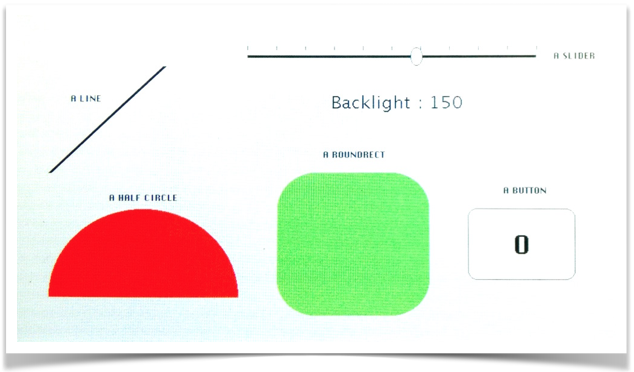
\includegraphics[width=6in]{AWFig1.png} 
   \caption{The AW\_doc\_example }
   \label{fig:1 }
\end{figure}


~\\Here is the complete listing : 

\begin{lstlisting}[language=Arduino]
//--- Project : ArduinoWidgets library
//--- Authors : Pierre Molinaro & Jean-Luc Bechennec
//--- Description : ArduinoWidgets library multiple views example 

#include <ArduinoWidgets.h>
#include <UTFT.h>

//--- This part is hardware dependent :
//--- Teensy 3.6 + LCD 7" with Touch, SSD1963 controler, resolution 800x480
//--- LCD type (see /Applications/Arduino.app/Contents/Java/hardware/teensy/avr/libraries/UTFT/UTFT.h)

static const byte RS    = 23 ;
static const byte WR    = 22 ;
static const byte CS    = 15 ;
static const byte RESET = 33 ;

//--- Warning D33 of Teensy 3.1: 
//--- https://forum.pjrc.com/threads/24823-Teensy-3-1-Tying-Pin-33-(pta4)-low-freezes-teensy

//--- Do not change 'myGLCD' name; it is declared as extern in AWContext.cpp

UTFT myGLCD (SSD1963_800ALT, RS, WR, CS, RESET) ;

static const byte T_CLK  = 11 ;
static const byte T_CS   = 12 ;
static const byte T_DIN  = 25 ;
static const byte T_DOUT = 24 ;
static const byte T_IRQ  = 28 ;

static const byte BACKLIGHT = 9 ;

//--- Do not change 'myTouch' name; it is declared as extern in AWContext.cpp
AWTouch myTouch (T_CLK, T_CS, T_DIN, T_DOUT, T_IRQ) ;

//--- end of hardware dependent part

////////////////////////////////////////////////////////////////
//--- Definitions of behaviours of existing Views in the library
////////////////////////////////////////////////////////////////

/////////////////////////// BUTTON /////////////////////////////

//--- button related global variable
int buttonValue = 0 ;

//--- button action
void bigButtonAction (AWView * inSender)
{
  AWPushButton * sendingButton = (AWPushButton *) inSender ;
  buttonValue ++ ;
  sendingButton->setTitle (String(buttonValue)) ;
  digitalWrite (LED_BUILTIN, !digitalRead(LED_BUILTIN));
}

//////////////// SLIDER //////////////////////

//--- Slider global variables
AWSlider *backlightSlider;
AWLabel * label1;   // constant label
AWLabel * label2;   // variable label
//--- Slider action
void sliderAction (AWView * inSender)
{
  AWSlider * sendingSlider = (AWSlider *) inSender ;
  AWInt pos = sendingSlider->knobPosition ();
  if (sendingSlider == backlightSlider) {
    analogWrite (BACKLIGHT, pos);
    label2->setTitle(pos);
  }
}

//////////////////////////////////////
//--- Definitions of new View classes 
//////////////////////////////////////

/////////////// ROUND CORNERS RECTANGLE ///////////////

class CustomView1 : public AWView
{
  CustomView1 (const AWRect & inViewFrame);
  virtual void drawInRegion (const AWRegion & inRegion) const;
};
CustomView1::CustomView1 (const AWRect & inViewFrame) :
AWView(inViewFrame, 
  AWColor ()),                  // let the corners opaque, outside the drawing region
  Color2 (AWColor::green ()) 
  { }
void CustomView1::drawInRegion (const AWRegion & inRegion) const
{
  AWRect viewFrame = absoluteFrame () ;
  AWContext::setColor (Color2) ;
  viewFrame.fillRoundRectInRegion (AWInt (50), inRegion) ; // radius of corners is 50
}
//--- Global variable ROUNDRECT
CustomView1 * roundRectView ;

///////////// CLIPPING VIEW : A HALF CIRCLE /////////////

class ClippingView : public AWView
{
  ClippingView (const AWRect & inViewFrame);
  virtual void drawInRegion (const AWRegion & inRegion) const;
};
ClippingView::ClippingView (const AWRect & inViewFrame) :
AWView(inViewFrame, 
  AWColor ())           // outside the drawing region is opaque 
  { }
void ClippingView::drawInRegion (const AWRegion & inRegion) const
{
  AWRegion drawingRegion = inRegion ;
  AWRect viewFrame = absoluteFrame () ;
  AWRect clipRectangle = viewFrame ;
  clipRectangle.size.width /= 1 ;
  clipRectangle.size.height /= 2 ;    // the clip rectangle hide the low half of the circle
  drawingRegion -= clipRectangle ;
  AWContext::setColor (AWColor::red ());
  viewFrame.fillOvalInRegion (drawingRegion) ;
}
//--- Global variable CLIPPING VIEW
ClippingView * crossView ;


/////////////////////// SETUP //////////////////////////////

void setup() {
//--- This part is hardware dependent
//--- set up the backlight
  analogWrite (BACKLIGHT, 150);
  pinMode (LED_BUILTIN, OUTPUT);
  digitalWrite (LED_BUILTIN, HIGH);

  AWContext::begin (kOrientationLandscape,
                    800,      // Screen width
                    480,      // Screen height
                    true,     // true : X is flipped
                    false) ;  // false : Y is not flipped

//--- end of hardware dependent part

//--- create a button on screen
  AWPushButton * bigButton = new AWPushButton(AWRect (600, 100, 140, 100), String (buttonValue), AWFont (ChicagoDigit36)) ;
  bigButton->setAction (bigButtonAction) ; 
  addView (new AWLabel (AWPoint (625, 220), 100, kAWAlignmentCenter, "A BUTTON")) ;
  addView (bigButton) ; 

//--- create 2 labels, one constant and one that can be changed by the slider 
  label1 = new AWLabel(AWPoint ( 300, 340), AWInt (250), AWAlignment (kAWAlignmentRight), String ("Backlight : "), AWFont (Lucida_Grande24)) ;
  addView (label1) ;
  label2 = new AWLabel(AWPoint ( 550, 340), AWInt (100), AWAlignment (kAWAlignmentLeft), String ("150"), AWFont (Lucida_Grande24)) ;
  addView (label2) ;

//--- create the slider with its label
  backlightSlider = new AWSlider (AWPoint (300,400), 400, kHorizontal, true) ;
  backlightSlider->setMaxKnobPosition (255);
  backlightSlider->setKnobPosition (150);
  backlightSlider->setAction (sliderAction);
  addView (new AWLabel (AWPoint (690, 410), 100, kAWAlignmentCenter, "A SLIDER")) ;
  addView (backlightSlider) ;

//--- create a black line of 5 pixel of thickness
  AWPoint lineOrigin ;
  lineOrigin.x = 50 ;
  lineOrigin.y = 250 ;
  AWPoint lineEnd;
  lineEnd.x = 200 ;
  lineEnd.y = 400 ;
  for (int i=0 ; i < 5 ; i++) {
    addView (new AWLine (lineOrigin, lineEnd)) ;
    lineOrigin.x++;
    lineEnd.x++;
  }
  addView (new AWLabel (AWPoint (50, 350), 100, kAWAlignmentCenter, "A LINE")) ;

//--- create the roundRect
  roundRectView = new CustomView1(AWRect (350, 50, 200, 200)) ;
  addView (roundRectView) ;   
  addView (new AWLabel (AWPoint (400, 270), 100, kAWAlignmentCenter, "A ROUNDRECT")) ;

//--- create the clipping view (half-circle)
  crossView = new ClippingView(AWRect (50, -50, 250, 250)) ;
  addView (crossView) ;
  addView (new AWLabel (AWPoint (100, 210), 150, kAWAlignmentCenter, "A HALF CIRCLE")) ;
  
  }

///////////////////////////// LOOP /////////////////

void loop() {
  AWContext::handleTouchAndDisplay () ;
}
\end{lstlisting}

~\\ To run this program, it is recommended to open the sketch in the example folder of the \emph{ArduinoWidgets} library, because a small file must be present in the same folder as the sketch. Its name must be "touch-calibration-values.h" and it must contain :

\begin{lstlisting}[language=Arduinonl]
#include "touch-calibration-values.h"

const float xA =  310.0 ; // 571.0 ;
const float yA =  116.0 ; // 963.0 ;

const float xB = 3811.0 ; // 488.0 ;
const float yB =  113.0 ; // 3001.0 ;

const float xC = 3814.0 ; // 3526.0 ;
const float yC = 3936.0 ; // 3349.0 ;

const float xD =  362.0 ; // 3519.0 ;
const float yD = 3938.0 ; // 698.0 ;
\end{lstlisting}

~\\ This .cpp file contain the values of the calibration of your screen.
If this file is not present in the sketch folder, a compilation error will occur

\begin{lstlisting}[language=Arduinonl]
.../AWContext.cpp:617: undefined reference to `yA'
.../AWContext.cpp:642: undefined reference to `xA'
.../AWContext.cpp:643: undefined reference to `yB'
.../AWContext.cpp:643: undefined reference to `yC'
.../AWContext.cpp:643: undefined reference to `xB'
.../AWContext.cpp:643: undefined reference to `yD'
.../AWContext.cpp:643: undefined reference to `xC'
.../AWContext.cpp:634: undefined reference to `xD'
\end{lstlisting}

~\\ Go to the section "Calibration" to know how to calibrate your touch screen.

%%%%%%%%%%%%%%%%%%%%%%%%%%%%%%%%%%%
\newpage
\section{A quick overview of the AW\_doc\_example}

~\\This section is not an in depth description on how to use each object of the library but just a global introduction to how to build a program which use the \emph{ArduinoWidgets} library. A detailed description of the library is given in the next sections of this document.

~\\ The program is divided in five parts :
\begin{itemize}
  \item The first part is to include the necessary libraries.
  \item The second part is the necessary adaptation to your hardware.
  \item The third part is the declaration of new graphic objets, the specific behaviors of existing objects of the library and the declarations of constants and variables.
  \item The fourth part is the setup() function in which there also a part for your specific hardware
  \item The fifth part is the loop() function.
\end{itemize}

~\\The first step is to import the two necessary libraries \emph{ArduinoWidgets} and \texttt{UTFT} .
\begin{lstlisting}[language=Arduinonl]
#include <ArduinoWidgets.h>
#include <UTFT.h>
\end{lstlisting}

~\\Before using your specific Touch LCD display, please read the following documents which are located inside the UTFT/documentation folder :

\begin{itemize}
\item  "UTFT\_Requirements.pdf" for describing the pins which are used to connect your micro-controller to your LCD 
 \item "UTFT\_Supported\_display\_modules\_\&\_controllers.pdf" for finding the right declaration of the controller which is used in your screen 
\end{itemize}

~\\Then adapt the hardware dependent part 1 in the listing to your specific hardware :
 
 \begin{lstlisting}[language=Arduinonl]
//--- This part is hardware dependent, such as here :
//--- Teensy 3.6 + LCD 7" with Touch, 
//--- SSD1963 controler, resolution 800x480

static const byte RS    = 23 ;
static const byte WR    = 22 ;
static const byte CS    = 15 ;
static const byte RESET = 33 ;

//--- Do not change 'myGLCD' name; 
//--- it is declared as extern in AWContext.cpp

UTFT myGLCD (SSD1963_800ALT, RS, WR, CS, RESET) ;

static const byte T_CLK  = 11 ;
static const byte T_CS   = 12 ;
static const byte T_DIN  = 25 ;
static const byte T_DOUT = 24 ;
static const byte T_IRQ  = 28 ;

static const byte BACKLIGHT = 9 ;

//--- Do not change 'myTouch' name; 
//--- it is declared as extern in AWContext.cpp

AWTouch myTouch (T_CLK, T_CS, T_DIN, T_DOUT, T_IRQ) ;

//--- end of hardware dependent part  
\end{lstlisting}

~\\ At this stage, dont forget to add the file "touch-calibration-values.h" which must be present in the same folder as the sketch (see the end of section 3).
  
~\\Then add the specific customizations and creations of the objets to display on the screen, with the desired interactivity :

\begin{itemize}
\item  a value to display inside a button and an action when clicking in the button, which increment the button's value; 
 \item some variables and an action to be attached to a slider which control the brightness of the backlight of the screen;
 \item a new AWView object to display a rectangle with round corners;
 \item a new AWView object to display a half circle which is the combination of a full circle with a clipping rectangle.
\end{itemize}

~\\Then the \texttt{setup()} function initialize the backlight of the LCD to the value 150 (the maximum is 255). 
~\\Then it initialize the LCD with the proper parameters (orientation, size, X and Y directions). Please note that the origine (0,0) of the screen is in the lower-left corner, exactly as in a Cartesian coordinate system.

~\\The objects are then created :

\begin{itemize}
\item  the button and its label; 
 \item two labels, one of which is associated to the action of the slider;
 \item the slider;
 \item a black line;
 \item the roundRect;
 \item the half circle;
\end{itemize}


\begin{lstlisting}[language=Arduinonl]
void setup() {
//--- This part is hardware dependent
//--- set up the backlight
  analogWrite (BACKLIGHT, 150);
  pinMode (LED_BUILTIN, OUTPUT);
  digitalWrite (LED_BUILTIN, HIGH);

  AWContext::begin (kOrientationLandscape,
                    800,      // Screen width
                    480,      // Screen height
                    true,     // true : X is flipped
                    false) ;  // false : Y is not flipped

//--- end of hardware dependent part

//--- create a button on screen
  AWPushButton * bigButton = new AWPushButton(AWRect (600, 100, 140, 100), String (buttonValue), AWFont (ChicagoDigit36)) ;
  bigButton->setAction (bigButtonAction) ; 
  addView (new AWLabel (AWPoint (625, 220), 100, kAWAlignmentCenter, "A BUTTON")) ;
  addView (bigButton) ; 

//--- create 2 labels, one constant and one that can be changed by the slider 
  label1 = new AWLabel(AWPoint ( 300, 340), AWInt (250), AWAlignment (kAWAlignmentRight), String ("Backlight : "), AWFont (Lucida_Grande24)) ;
  addView (label1) ;
  label2 = new AWLabel(AWPoint ( 550, 340), AWInt (100), AWAlignment (kAWAlignmentLeft), String ("150"), AWFont (Lucida_Grande24)) ;
  addView (label2) ;

//--- create the slider with its label
  backlightSlider = new AWSlider (AWPoint (300,400), 400, kHorizontal, true) ;
  backlightSlider->setMaxKnobPosition (255);
  backlightSlider->setKnobPosition (150);
  backlightSlider->setAction (sliderAction);
  addView (new AWLabel (AWPoint (690, 410), 100, kAWAlignmentCenter, "A SLIDER")) ;
  addView (backlightSlider) ;

//--- create a black line of 5 pixel of thickness
  AWPoint lineOrigin ;
  lineOrigin.x = 50 ;
  lineOrigin.y = 250 ;
  AWPoint lineEnd;
  lineEnd.x = 200 ;
  lineEnd.y = 400 ;
  for (int i=0 ; i < 5 ; i++) {
    addView (new AWLine (lineOrigin, lineEnd)) ;
    lineOrigin.x++;
    lineEnd.x++;
  }
  addView (new AWLabel (AWPoint (50, 350), 100, kAWAlignmentCenter, "A LINE")) ;

//--- create the roundRect
  roundRectView = new CustomView1(AWRect (350, 50, 200, 200)) ;
  addView (roundRectView) ;   
  addView (new AWLabel (AWPoint (400, 270), 100, kAWAlignmentCenter, "A ROUNDRECT")) ;

//--- create the clipping view (half-circle)
  crossView = new ClippingView(AWRect (50, -50, 250, 250)) ;
  addView (crossView) ;
  addView (new AWLabel (AWPoint (100, 210), 150, kAWAlignmentCenter, "A HALF CIRCLE")) ;
  
  }
  \end{lstlisting}

~\\The \texttt{loop()} function of the sketch is very simple since it contain only one instruction which do everything : get events and call actions: \texttt{handleTouchAndDisplay()} \\
 
\begin{lstlisting}[language=Arduinonl]
void loop() {
  AWContext::handleTouchAndDisplay () ;
}  
\end{lstlisting}
  
%%%%%%%%%%%%%%%%%%%%%%%%%%%%%%%%%%%
\newpage
\subsection{How to use the code lines of the following sections of \emph{ArduinoWidgets}}

~\\In the following sections of this document, there is three pieces of Arduino code that will not be repeated.

~\\The first one is :
\begin{lstlisting}[language=Arduinonl]
#include <ArduinoWidgets.h>
#include <UTFT.h>
//--- This part is hardware dependent, such as here :
//--- Teensy 3.6 + LCD 7" with Touch, 
//--- SSD1963 controler, resolution 800x480

static const byte RS    = 23 ;
static const byte WR    = 22 ;
static const byte CS    = 15 ;
static const byte RESET = 33 ;

//--- Do not change 'myGLCD' name; 
//--- it is declared as extern in AWContext.cpp

UTFT myGLCD (SSD1963_800ALT, RS, WR, CS, RESET) ;

static const byte T_CLK  = 11 ;
static const byte T_CS   = 12 ;
static const byte T_DIN  = 25 ;
static const byte T_DOUT = 24 ;
static const byte T_IRQ  = 28 ;

static const byte BACKLIGHT = 9 ;

//--- Do not change 'myTouch' name; 
//--- it is declared as extern in AWContext.cpp

AWTouch myTouch (T_CLK, T_CS, T_DIN, T_DOUT, T_IRQ) ;

//--- end of hardware dependent part 

//--- add here you constants, classes, functions, variables, ...
\end{lstlisting}

~\\The second one is  the \texttt{setup()} :
\begin{lstlisting}[language=Arduinonl]
void setup() {
//--- This part is hardware dependent
//--- set up the backlight
  analogWrite (BACKLIGHT, 150);
  pinMode (LED_BUILTIN, OUTPUT);
  digitalWrite (LED_BUILTIN, HIGH);

  AWContext::begin (kOrientationLandscape,
                    800,      // Screen width
                    480,      // Screen height
                    true,     // true : X is flipped
                    false) ;  // false : Y is not flipped

//--- end of hardware dependent part

//--- add here your lines of code for setup

} //--- end of setup
\end{lstlisting}

~\\The third par is the \texttt{loop()} function of the sketch.
 
\begin{lstlisting}[language=Arduinonl]
void loop() {
  AWContext::handleTouchAndDisplay () ;
}  
\end{lstlisting}
~\\You can create an Arduino sketch by inserting first the 3 parts above, then the lines of code found in the various examples below.
  
~\\If you want to test the examples which are described in this document, the best way is to use the "example" menu of the Arduino's IDE. But you can also assemble the lines of code of each subsection with the above parts to be adapted first to you specific hardware.
  
%%%%%%%%%%%%%%%%%%%%%%%%%%%%%%%%%%%
\newpage
\section{The fondation of \emph{ArduinoWidgets}}

~\\The \emph{ArduinoWidgets} library is objet oriented (C++). It is made of a collection of classes the instances of which are objects. The collection of classes can be expanded later in future versions and you can create your own classes with inheritance.

~\\The consequence is the naming and the syntax to use in your Arduino program : 
\begin{itemize}
\item Objects are instances of class.
\item Each class embed its own variables which are hidden to your sketch and class variables which are independent of objects
\item Each class also embed functions which concern one objects and are public for use by your code, and also class functions which are independent of objects.
\end{itemize}

~\\For example, drawing a line consists to create an instance of a AWLine class  :

\begin{lstlisting}[language=Arduinonl]
AWLine * myLine;
  myLine = new AWLine (AWPoint(100,100), AWPoint(300,300)); 
  addView (myLine) ;
 \end{lstlisting}


~\\ The object myLine (a pointer) is an instance of the AWLine class, which is a line to draw between 2 points of coordinate (100,100) and (300, 300) with the constructor \texttt{new AWLine}.
~\\ The class function \texttt{addView} just add the drawing of the line to the list of drawings. The effective drawing will be made by the class function \texttt{handleTouchAndDisplay} which is called once for all drawings, in the loop.

~\\ Another example is the display of a text label :

\begin{lstlisting}[language=Arduinonl]
  label = new AWLabel(AWPoint ( 300, 340), AWInt (150), AWAlignment (kAWAlignmentCenter), String ("My Label : "), AWFont (Lucida_Grande24)) ;
  addView (label) ;
\end{lstlisting}

~\\ The object \texttt{label} is created with the constructor of the class \texttt{AWLabel}, with the parameters which define the coordinate and size of the text field, the default string in it and the font. The class function addView just add the drawing of the line to the list of drawings as explained above.


%%%%%%%%%%%%%%%%%%%%
\newpage
\subsection{Context}

~\\ The \emph{Context} is the entire Screen you are using. You must know about \emph{Context} before seeing something on your screen and touch it. 
~\\ To create a context, just call the \texttt{begin} function of class \texttt{AWContext}. This must be done only once in your sketch.

~\\ For example :

\begin{lstlisting}[language=Arduinonl]
 AWContext::begin (kOrientationLandscape,
                    800,      // Screen width
                    480,      // Screen height
                    true,     // true : X is flipped
                    false) ;  // false : Y is not flipped
\end{lstlisting}

~\\ This describe the specific display which is in use : landscape orientation, dimensions : 800x600, horizontal axis is flipped, not the vertical axis.

~\\ The orientation can be either \texttt{kOrientationLandscape}, \texttt{kOrientationPortrait}.

~\\ There is a method in the \texttt{loop} for dealing with all events and actions of the touch screen and the draw and redraw on the screen according to the events. This is the unique instruction in the \texttt{loop} which work as a background task in the examples.

\begin{lstlisting}[language=Arduinonl]
  static void handleTouchAndDisplay (void) ;
\end{lstlisting}

~\\ \texttt{handleTouchAndDisplay} handle the touch events, especially the press detection (touchDown), press move (touchMove), press release (touchUp), and the drawing of all views (see View section) on the screen. Generally, a touch event generate an action which is sent to a specific object in a view.

~\\ The \emph{Context} have also a variety of properties and methods, such as :

\begin{itemize}
\item A screen rectangle : you can get the size on the screen rectangle
\begin{lstlisting}[language=Arduinonl]
//--- Screen rect
  static AWRect screenRect (void) ;
\end{lstlisting}

\item A color (backgroung color) : you can set or get the color of the screen and its opacity
\begin{lstlisting}[language=Arduinonl]
//--- Color
  static void setColor (const AWColor & inColor) ;
  static AWColor color (void) ;
  static bool colorIsOpaque (void) ;
\end{lstlisting}

\item A calibration method  with the drawing of a calibration rectangle and specific points to touch: 
\begin{lstlisting}[language=Arduinonl]
static void calibrateTouch (void) ;
\end{lstlisting}

\end{itemize}

%%%%%%%%%%%%%%%%%%%%%%
\newpage
\subsection{The Views}

~\\ Every pieces of drawing on the screen are "Views".
~\\ A view is a rectangular section of the screen. It is responsible for handling all drawing and user-initiated events within its frame.

~\\ \emph{ArduinoWidgets} provides the \texttt{View} class as an abstract view implementation that subclasses use as the basis for implementing custom display and user interaction. They are the most pervasive type of object in the \emph{ArduinoWidgets} library; nearly every object you see on the screen is a view. Views are in the front line of both drawing and event handling, and hence are one of the more important types of objects to understand.
~\\ In a very real sense, a view draws itself. It also provides a surface that can be responsive to input from a touch event.

~\\ In addition to drawing content and responding to user events, \texttt{View} instances act as containers for other views. By nesting views within other views, an application creates a hierarchy of views. This view hierarchy provides a clearly defined structure for how views draw relative to each other and pass messages from one view to another, up to the enclosing window, and on to the application for processing.

~\\ \emph{ArduinoWidgets} provides several type of views for containing graphics, texts and controls, with color attributes, which can send messages to its own view or to other views. A view can be opaque or transparent. In this last case, if the view is not validated, the drawing of views behind it is allowed.

~\\ The root \texttt{View} is the screen.
~\\ Each \texttt{View} is placed in a parent View, the \texttt{superView}, in which it is a frame. This frame can be moved and resized in the \texttt{superView} and the view's content moves with it.

~\\ The view is specified when a view instance is created programmatically using :

\begin{lstlisting}[language=Arduinonl]
//--- Constructor
  AWView (const AWRect & inRelativeFrame,
                   const AWColor & inBackColor) ;
 \end{lstlisting}

~\\ When it is necessary to know the frame rectangle of a view, the \texttt{absoluteFrame} method can return this frame rectangle.

~\\ To translate a frame you can use the method \texttt{translateBy}. To change the frame size you can use \texttt{setSize}.
~\\ To specify or to get the backcolor of a view, you can use the methods \texttt{backColor} or \texttt{setBackColor}.

\begin{lstlisting}[language=Arduinonl]
//---------------- Frame
  inline AWRect absoluteFrame (void) const { return mAbsoluteFrame ; }

//---------------- Frame change
  void translateBy (const AWInt inDx, const AWInt inDy) ;
  void setSize (const AWSize & inNewSize) ;

//---------------- Background color
  inline AWColor backColor (void) const { return mBackColor ; }
  void setBackColor (const AWColor & inBackColor) ;
\end{lstlisting}

~\\ To add a new View on the screen, just call \texttt{addView} or \texttt{addCenteredView} :
\begin{lstlisting}[language=Arduinonl]
void addView (class AWView * inView) ;
void addCenteredView (class AWView * inView) ;
\end{lstlisting}

~\\\emph{What is a View Hierarchy?}

~\\In addition to being responsible for drawing and handling user events, a view instance can act as a container, enclosing other view instances. Those views are linked together creating a view hierarchy. Unlike a class hierarchy, which defines the lineage of a class, the view hierarchy defines the layout of views relative to other views.

~\\ It permits a complex view to be constructed out of other views. For example, a graphical keypad might be a container view with a separate subview for each key.

~\\The \texttt{context} instance maintains a reference to a single top-level view instance. \texttt{addView} and addCenteredView without argument just add a subview to the root view.

~\\The view instances enclosed within a view are called subViews. The parent view that encloses a view is referred to as its \texttt{superView}. Each view has another view as its superView and may be the superView for any number of subViews. While a view instance can have multiple subViews, it can have only one superView. In order for a view and its subviews to be visible to the user, the view must be inserted into a view hierarchy.

~\\ A view is added to a parent view via the method \texttt{addSubView} or \texttt{addCenteredSubView}, in a hierarchical order :
\begin{lstlisting}[language=Arduinonl]
//---------------- Managing view hierarchy
  void addSubView (AWView * inView) ;         // if inView is non NULL, view is added in front of other subviews
  void addCenteredSubView (AWView * inView) ; // if inView is non NULL, view is added in front of other subviews
\end{lstlisting}


~\\To locate the superView use the method \texttt{superViev}. You can also remove a subView from a superView with \texttt{removeFromSuperView}.

\begin{lstlisting}[language=Arduinonl]
//---------------- Managing view hierarchy
  void addSubView (AWView * inView) ;         // if inView is non NULL, view is added in front of other subviews
  void addCenteredSubView (AWView * inView) ; // if inView is non NULL, view is added in front of other subviews
  void removeFromSuperView (void) ; // Does nothing if has no super view
  inline AWView * superView (void) { return mSuperView ; } // Returns NULL if has no super view
\end{lstlisting}

~\\ An example of a View containing subViews will be given in subsection "PushButton".

~\\\emph{View Tags}

~\\The View class defines methods that allow you to tag individual view objects with integer tags.

~\\The View method \texttt{tag} always returns –1. Subclasses can override this method to return a different value. It is common for a subclass to implement a \texttt{setTag} method that stores the tag value in an instance variable, allowing the tag to be set on an individual view basis. 

\begin{lstlisting}[language=Arduinonl]
//---------------- Tag
  inline void setTag (const int inTag) { mTag = inTag ; }
  inline int tag (void) const { return mTag ; }
\end{lstlisting}

~\\ \emph{User interactivity : sending and receiving Actions}

~\\A view or subview can be sensitive to touch actions of the user. In order to be responsive to a touch event, each view must redefine \texttt{touchDown}, \texttt{touchMove} and \texttt{touchUp}. The method \texttt{sendAction} call the function which is attached to the view by using \texttt{setAction} :

\begin{lstlisting}[language=Arduinonl]
//---------------- Action
  void sendAction (void) ;
  inline AWAction action (void) const { return mAction ; }
  inline void setAction (AWAction inAction) { mAction = inAction ; }

//---------------- Touch
  virtual void touchDown (const AWPoint & inPoint) ;
  virtual void touchMove (const AWPoint & inPoint) ;
  virtual void touchUp (const AWPoint & inPoint) ;
\end{lstlisting}

~\\ \emph{Drawing and display views}
~\\ These methods force a display of the screen by the function \texttt{handleTouchAndDisplay}, although the later method iterates only through the list of invalidated views. The display method causes each view in the screen's view hierarchy to redraw itself. 

~\\ These methods mark views or regions of views for redrawing 
:
\begin{lstlisting}[language=Arduinonl]
//---------------- Display view
  void setNeedsDisplay (void) ;
  void setNeedsDisplayInRect (const AWRect & inRect) ;
\end{lstlisting}

~\\ The method \texttt{drawInRegion} may be redefined in each view : It is responsible of the drawing of the view.

\begin{lstlisting}[language=Arduinonl]
//--- Draw method (to be overridden)
  virtual void drawInRegion (const AWRegion & inDrawRegion) const ;
\end{lstlisting}

~\\ A view can be opaque (visible) or transparent (invalid or invisible). An important aspect of the drawing of views is view opacity. A view does not have to draw every bit of its surface, but if it does it should declare itself to be opaque (by implementing isOpaque to return YES).

\begin{lstlisting}[language=Arduinonl]
//--- Tell the view is opaque
  virtual bool isOpaque (void) const ;

//---------------- Visibility
  inline bool isVisible (void) const { return mIsVisible ; }
  void setVisibility (const bool inIsVisible) ;

//---------------- Handle "on screen" state
  inline bool isOnScreen (void) const { return mIsOnScreen ; }
\end{lstlisting}


~\\ \texttt{AWView} is a class that defines the basic drawing and event-handling. \texttt{AWView} itself does not draw content or respond to user events, so you typically don’t interact with a direct instance of \texttt{AWView}. Instead you use an instance of a custom \texttt{AWView} subclass. A custom view class inherits from \texttt{AWView} and overrides many of its methods, which are invoked automatically by the \emph{ArduinoWidgets} library.

~\\ There is a collection of ready to use subclass Views in the \emph{ArduinoWidgets} library, which are :
\begin{itemize}
\item \texttt{AWLine} : display a line
\item \texttt{AWLabel} : display of text on a line.
\item \texttt{AWPushButton} : display a button
\item \texttt{AWRectView} : display a rectangle with or without round corners
\item \texttt{AWSegmentedControl} : display a radio button in a tab form
\item \texttt{AWSlider} : display a linear potentiometer with one cursor
\item \texttt{AWDynamicSlider} : display a linear potentiometer with one cursor
\item \texttt{AWTabview} : display tabs which are usefull for switching from one View to another. 
\item \texttt{AWSwitch} : display a check box. 
\item \texttt{AWArrowPushButton} : display a button with an arrow shape. 
\item \texttt{AWKeyButton} : display a key of keyboard 
\item \texttt{AWKeyboardBackView} : display an entire keyboard. 
\end{itemize}

~\\ You also will be able to create and add your custom View !

%%%%%%%%%%%%%%%%%%%%%%%%%%%%%%%%%%%
\newpage
\subsection{The action}

~\\ The action is the interactive part of the \emph{ArduinoWidgets} library, which rely on the touch capabilities of the screen. An action is the message a control sends to the target or, from the perspective of the target, the method it implements to respond to the action. 

~\\The standard way to pass information between objects is message passing—one object invokes the method of another object. However, message passing requires that the object sending the message know who the receiver is and what messages it responds to. This is the reason why the action routines are located in the declaration part of the Arduino sketch, before the \texttt{setup}.

~\\ A control is a view object which implement touch capabilities. For exemple, \texttt{myControl} (a PushButton or a Key or a Tab, for example) is a control. In the \texttt{setup}, inside the initialization code of \texttt{myControl}, we add the following line :

\begin{lstlisting}[language=Arduinonl]
myControl->setAction (myControlAction) ;
\end{lstlisting}

~\\ \texttt{myControlAction} is a routine which is declared before the setup. We suppose here that this control is, for example, a PushButton :

\begin{lstlisting}[language=Arduinonl]
//--- myControl action
void myControlAction (AWView * inSender)
{
  AWPushButton * sendingButton = (AWPushButton *) inSender ;
  // Your Action code here
}
\end{lstlisting}

~\\ Your action code can display  a label's title, control any Arduino's output pin (a led, a PWM signal, the backlight of the screen, etc..).
~\\ You will find several example of how an action is implemented in the description of the following \emph{ArduinoWidgets} views.

%%%%%%%%%%%%%%%%%%%%%%%%%%%%%%%%%%
\newpage
\subsection{The coordinate plane}

~\\ A view is responsible for the drawing and event handling in a rectangular area of a window. In order to specify that rectangle of responsibility, you define its location as an origin point and size using a coordinate system.
~\\This section describes the coordinate system used by views, how a view's location and size is specified, and how the size of a view interacts with its content.

~\\ All information about location is given to \emph{ArduinoWidgets} in terms of coordinates on a plane. The coordinate plane is a two-dimensional grid, as illustrated in Figure 2.

\begin{figure}[htbp]
   \centering
   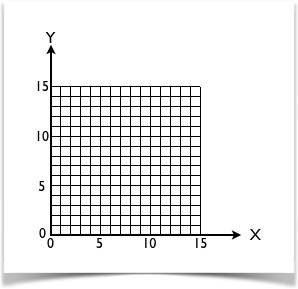
\includegraphics[scale=1]{AWFig2.png} 
   \caption{The coordinate plane}
   \label{fig:2 }
\end{figure}

~\\All grid coordinates are AWInt (in the range -32767 to 32767).

\begin{lstlisting}[language=Arduinonl]
typedef int16_t AWInt ;
\end{lstlisting}

~\\The origine of all coordinates is (0,0) and is located at the bottom left corner of the screen.
~\\ Note that  the \texttt{begin} function of class \texttt{AWContext} have 2 boolean parameters to flip or not the X and Y coordinates if necessary.
~\\Horizontal coordinates increase as you move from left to right, and vertical coordinates increase as you move from bottom to top. 

~\\ Each view use the same coordinate system as its mother view. 



%%%%%%%%%%%%%%%%%%%%
\newpage
\subsection{Points and Pixels}

~\\Each point is at the intersection of a horizontal grid line and a vertical grid line. 
~\\The coordinate origin (0,0) is in the lower-left corner of the screen. 

~\\You can store the coordinates of a point into an object \texttt{AWPoint} which contain 2 variables of type AWInt :

\begin{lstlisting}[language=Arduinonl]
// AWPoint :
  AWInt x ;
  AWInt y ;
\end{lstlisting}

~\\Figure 3 shows the relationship between points, grid lines, and pixels, the physical dots on the screen. 
A pixel is centered around a point. In other words, a point is at the center of a pixel.

\begin{figure}[htbp]
   \centering
   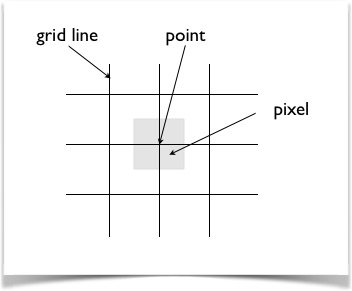
\includegraphics[scale=0.8]{AWFig3.png} 
   \caption{Points and Pixels}
   \label{fig:3 }
\end{figure}


~\\To create a \texttt{AWPoint} at coodinates X and Y, you call :
\begin{lstlisting}[language=Arduinonl]
AWPoint myPoint  ;
myPoint.x = X;
myPoint.y = Y;
\end{lstlisting}

~\\ The Point is not a View. The above \texttt{myPoint} is not drawed at this stage.

~\\ To compare two Points there is two special operators :
\begin{lstlisting}[language=Arduinonl]
//--- Equatable
  inline bool operator == (const AWPoint & inP) const { return (x == inP.x) && (y == inP.y) ; }
  inline bool operator != (const AWPoint & inP) const { return !(*this == inP) ; }
\end{lstlisting}

~\\ The Point class has the following methods : (?? Why and how to use it ??)

\begin{lstlisting}[language=Arduinonl]
//--- Translation
  void translateBy (const AWInt inDx, const AWInt inDy) { x += inDx ; y += inDy ; }
  void translateBy (AWPoint & inTranslation) { x += inTranslation.x ; y += inTranslation.y ; }

//--- Stroke line
  void strokeLineInRegion (const AWPoint & inPoint, const AWRegion & inDrawRegion) const ;

  static void strokeLineInRegion (const AWInt inP1X,
                                           const AWInt inP1Y,
                                           const AWInt inP2X,
                                           const AWInt inP2Y,
                                           const AWRegion & inDrawRegion) ;

//--- Draw Point
  void drawInRegion (const AWRegion & inDrawRegion) const ;
  static void drawPointInRegion (const AWInt inX, const AWInt inY, const AWRegion & inDrawRegion) ;
\end{lstlisting}

~\\ And a special drawing of circle (?? Why and how to use it ??)

\begin{lstlisting}[language=Arduinonl]
//--- Frame circle
  void frameCircleInRegion (const AWInt inRadius,
               const AWRegion & inDrawRegion) const ;

  static void frameCircleInRegion (const AWInt inCenterX,
            const AWInt inCenterY,
            const AWInt inRadius,
            const AWRegion & inDrawRegion) ;

//--- Fill circle
  void fillCircleInRegion (const AWInt inRadius,
            const AWRegion & inDrawRegion) const ;

   static void fillCircleInRegion (const AWInt inCenterX,
             const AWInt inCenterY,
             const AWInt inRadius,
             const AWRegion & inDrawRegion) ;
\end{lstlisting}

%%%%%%%%%%%%%%%%%%%%%%%%%%%%%%%%%%%%%%%%%%%%%%
\newpage
\subsection{Rectangle}

~\\ A rectangle is not a View but a rectangle is the fondation of each \texttt{AWView}.

~\\ A Rectangle is defined by an origine \texttt{AWPoint} and an \texttt{AWsize}. The origine Point is the bottom-left corner :

\begin{lstlisting}[language=Arduinonl]
//--- Properties
  AWPoint origin ;
  AWSize size ;
  
// AWsize :
AWInt width ;
AWInt height ;

// AWRect :
myRect = new AWRect (AWPoint, AWSize);
myRect = new AWRect (X, Y, width, height);
\end{lstlisting}

~\\The coordinates of the bottom left corner are X = left, Y = bottom.
~\\ For example, you can create a new rectangle \texttt{myRect} of left-bottom corner X=350, Y=50, width W=200 and height H=200 like this :
\begin{lstlisting}[language=Arduinonl]
myRect = new AWRect (350, 50, 200, 200);
\end{lstlisting}

\begin{figure}[htbp]
   \centering
   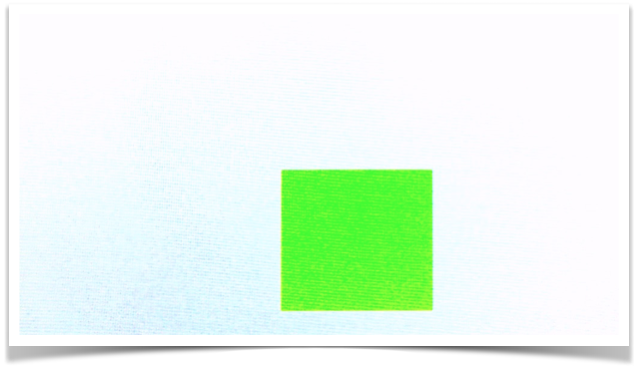
\includegraphics[scale=0.7]{AWFig6.png} 
   \caption{A Rectangle}
   \label{fig:6 }
\end{figure}

~\\ This rectangle have a bottom left corner origin of coordinates (350, 50).
~\\ The width (200) and height (200) are the number in pixels in the horizontal and vertical directions.

~\\ Consequently, the coordinate of the top right corner of this rectangle is (549, 249) :
\begin{itemize}
\item left = X = 350
\item bottom = Y = 50
\item right = X + W -1 = 350 + 200 -1 = 549
\item top = Y + H -1 = 50 + 200 -1 = 249
\end{itemize}


~\\ You can create rectangle from various combinations of AWInt, AWPoint and AWSize, according to the 3 constructors. 

~\\ You will see farther all the operations and transformations that you can do on AWRect such as :
\begin{itemize}
\item to be visible or invisible or empty (if W <=0 or H <=0)
\item a pixel is a rectangle with W = H =1
\item a horizontal line is a rectangle with W =1
\item a vertical line is a rectangle with H = 1
\item a 800x600 screen is a rectangle (0, 0, 800, 600)
\item find corners points
\item make intersection, inclusion or union of rectangles
\item find differences (the opposite of intersection) of rectangles
\item inset en translate rectangles
\item draw and fill rectangles, round-rectangles, and ovales
\end{itemize}

~\\The following example show how to display two rectangles : one without round corners and one with round corners :

~\\ First declare custom Views based on respective rectangles. The new classes are RectangleView and RoundRectangleView. Then create an instance of each class :

\begin{lstlisting}[language=Arduinonl]
/////////////// RECTANGLE ///////////////
class RectangleView : public AWView
{
  RectangleView (const AWRect & inViewFrame);
  virtual void drawInRegion (const AWRegion & inRegion) const;
};
RectangleView::RectangleView (const AWRect & inViewFrame) : // constructor
AWView(inViewFrame, 
  AWColor ()),             
  RectColor (AWColor::orange ()) 
  { }
void RectangleView::drawInRegion (const AWRegion & inRegion) const
{
  AWRect viewFrame = absoluteFrame () ;
  AWContext::setColor (RectColor) ;
  viewFrame.fillRectInRegion (inRegion) ;
}
//--- Global variable RectView
RectangleView * RectView ;

/////////////// ROUND CORNERS RECTANGLE ///////////////
class RoundRectangleView : public AWView
{
  RoundRectangleView (const AWRect & inViewFrame);
  virtual void drawInRegion (const AWRegion & inRegion) const;
};
RoundRectangleView::RoundRectangleView (const AWRect & inViewFrame) : // constructor
AWView(inViewFrame, 
  AWColor ()),             
  RectColor (AWColor::green ()) 
  { }
void RoundRectangleView::drawInRegion (const AWRegion & inRegion) const
{
  AWRect viewFrame = absoluteFrame () ;
  AWContext::setColor (RectColor) ;
  viewFrame.fillRoundRectInRegion (AWInt (50), inRegion) ;
}
//--- Global variable RoundRectView
RoundRectangleView * RoundRectView ;
\end{lstlisting}

~\\ Then draw the rectangles in the setup() :

\begin{lstlisting}[language=Arduinonl]
  //--- draw the Rectangle
  RectView = new RectangleView (AWRect (350, 50, 200, 300)) ;
  addView (RectView) ;   
  
  //--- draw the RoundRectangle
  RoundRectView = new RoundRectangleView (AWRect (80, 200, 250, 200)) ;
  addView (RoundRectView) ;   
\end{lstlisting}

\begin{figure}[htbp]
   \centering
   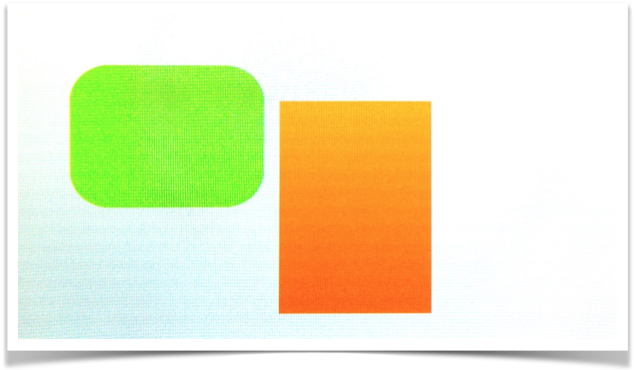
\includegraphics[scale=0.7]{AWFig7.png} 
   \caption{Two Rectangles}
   \label{fig:7}
\end{figure}

~\\ Figure 5 show these 2 rectangles.

~\\ 

~\\ There is a collection of operations on rectangles that are useful to know for drawing :

\begin{enumerate}
\item First, the class AWRect have a variety of constructors :

\begin{lstlisting}[language=Arduinonl]
  inline AWRect (const AWPoint inOrigin, const AWSize inSize) : origin (inOrigin), size (inSize) {}
  
  inline AWRect (const AWPoint inOrigin) : origin (inOrigin), size (AWSize (1, 1)) {}
  
  inline AWRect (const AWInt inX, const AWInt inY, const AWInt inWidth, const AWInt inHeight) :
  	origin (AWPoint (inX, inY)),
  	size (AWSize (inWidth, inHeight)) {}
	
  AWRect (const AWPoint & inP1, const AWPoint & inP2) ;
  
  static AWRect horizontalLine (const AWInt inX, const AWInt inY, const AWInt inWidth) ;
  
  static AWRect verticalLine (const AWInt inX, const AWInt inY, const AWInt inHeight) ;
\end{lstlisting}

\item Second, you can access the Point and Size values of a rectangle :

\begin{lstlisting}[language=Arduinonl]
  inline bool isEmpty (void) const { return (size.width <= 0) || (size.height <= 0) ; }
  bool containsPoint (const AWPoint & inPoint) const ;
  AWPoint topRight (void) const ;
  AWPoint bottomRight (void) const ;
  AWPoint topLeft (void) const ;
  inline AWPoint bottomLeft (void) const { return origin ; }
  inline AWInt minX (void) const { return origin.x ; }
  inline AWInt maxX (void) const { return origin.x + size.width - 1 ; }
  inline AWInt minY (void) const { return origin.y ; }
  inline AWInt maxY (void) const { return origin.y + size.height - 1 ; }
\end{lstlisting}

\item You can determine the intersection between 2 rectangles, which is a rectangle :

\begin{lstlisting}[language=Arduinonl]
  AWRect operator & (const AWRect & inOtherRect) const ;
  bool intersects (const AWRect & inOtherRect) const ;
\end{lstlisting}

\item You can determine the inclusion of 2 rectangles, which is a rectangle drawned around the included rectangles :

\begin{lstlisting}[language=Arduinonl]
  bool includesRect (const AWRect & inOtherRect) const ;
\end{lstlisting}

\item You can determine the union of 2 rectangles, which returns the smallest rectangle that completely encloses both receiver rect and inOtherRect :

\begin{lstlisting}[language=Arduinonl]
  AWRect operator + (const AWRect & inOtherRect) const ;
  void operator += (const AWRect inOtherRect) ;
\end{lstlisting}

\item You can determine the difference between 2 rectangles, which returns 4 rectangles, possibly empty :

\begin{lstlisting}[language=Arduinonl]
  void differenceFrom (const AWRect & inRect,
                                AWRect & outR1,
                                AWRect & outR2,
                                AWRect & outR3,
                                AWRect & outR4) const ;
\end{lstlisting}

\item You can transform a rectangle, by reducing its size or translating its coordinates :

\begin{lstlisting}[language=Arduinonl]
  void inset (const AWInt inDx, const AWInt inDy) ;
  void translateBy (const AWInt inDx, const AWInt inDy) ;
\end{lstlisting}

\item You can test the equality of 2 rectangles :

\begin{lstlisting}[language=Arduinonl]
//--- Equatable
  bool operator == (const AWRect & inRect) const { return (origin == inRect.origin) && (size == inRect.size) ; }
  inline bool operator != (const AWRect & inRect) const { return ! (*this == inRect) ; }
\end{lstlisting}

\item You have a series of  drawing a rectangle in regions which are explained below :
\end{enumerate}

\begin{lstlisting}[language=Arduinonl]
  void fillRectInRegion (const AWRegion & inDrawRegion) const ;
  void frameRectInRegion (const AWRegion & inDrawRegion) const ;
  void fillRoundRectInRegion (const AWInt inRadius, const AWRegion & inDrawRegion) const ;
  void frameRoundRectInRegion (const AWInt inRadius, const AWRegion & inDrawRegion) const ;
  void fillOvalInRegion (const AWRegion & inDrawRegion) const ;
  void frameOvalInRegion (const AWRegion & inDrawRegion) const ;
\end{lstlisting}

%%%%%%%%%%%%%%%%%%%%%%%%%%%%%%%%%%%%%%%%%%%%%%
\newpage
\subsection{Region}

~\\ The minimum Region is a Rectangle or can be empty.
~\\ A Region is made of a combination of one or more separate and non-empty rectangles.
~\\ The role of a Region is to manage more or less complex geometric entities which are not limited to a Rectangle.

~\\ A Region is not a View and do not allow any drawing by itself, but it allow several operations.

\begin{lstlisting}[language=Arduinonl]
//--- Region from a rectangle (empty if rectangle is empty)
 AWRegion (const AWRect & inRect) ; 
 AWRegion(); // build an empty region
\end{lstlisting}
  
~\\ The purpose of regions is to limit drawing within the region. 
~\\ For example, if you want to draw a half circle on the screen, you can set the region to half the square that enclose the whole circle, and then draw the whole circle. Only the half within the region will actually be drawn.

~\\ This is how is implemented this example :

~\\ First declare a custom View with a new class named \texttt{ClippingView} which derive from the class \texttt{AWViev}:

\begin{lstlisting}[language=Arduinonl]
///////////// CLIPPING VIEW : A HALF CIRCLE /////////////
class ClippingView : public AWView
{
  ClippingView (const AWRect & inViewFrame);
  virtual void drawInRegion (const AWRegion & inRegion) const;
};
ClippingView::ClippingView (const AWRect & inViewFrame) :
  AWView(inViewFrame, 
  AWColor ())           // outside the drawing region is opaque 
  { }
void ClippingView::drawInRegion (const AWRegion & inRegion) const
{
  AWRegion drawingRegion = inRegion ;
  AWRect viewFrame = absoluteFrame () ;
  AWRect clipRectangle = viewFrame ;
  clipRectangle.size.width /= 1 ;
  clipRectangle.size.height /= 2 ;    // the clip rectangle hide the low half of the circle
  drawingRegion -= clipRectangle ;
  AWContext::setColor (AWColor::red ());
  viewFrame.fillOvalInRegion (drawingRegion) ;
}
//--- Global variable CLIPPING VIEW
ClippingView * crossView ;
\end{lstlisting}

~\\ This \texttt{ClippingView} class inherit from the \texttt{AWView} class (variables and methods) and declare its constructor and the \texttt{drawInRegion} function.
~\\ This \texttt{drawInRegion} function determine the region which match the rectangle given in the constructor and build a clip rectangle (the half bottom of the region here) which is used to reduce the drawing region with the function \texttt{drawingRegion -= clipRectangle ;}.
~\\ Then a circle is drawn in the drawing region. The result will be a half circle !

~\\ The custom View is created in the \texttt{setup}  and displayed by the \texttt{handleTouchAndDisplay} function in the \texttt{loop}:
\begin{lstlisting}[language=Arduinonl]
//--- create the clipping view (half-circle
  crossView = new ClippingView(AWRect (300, 100, 250, 250)) ;
  addView (crossView) ;
\end{lstlisting}

~\\ The region is defined by a rectangle which extends from the bottom left corner (300, 100) with size (250, 250). The circle is centered in this rectangle.

\begin{figure}[htbp]
   \centering
   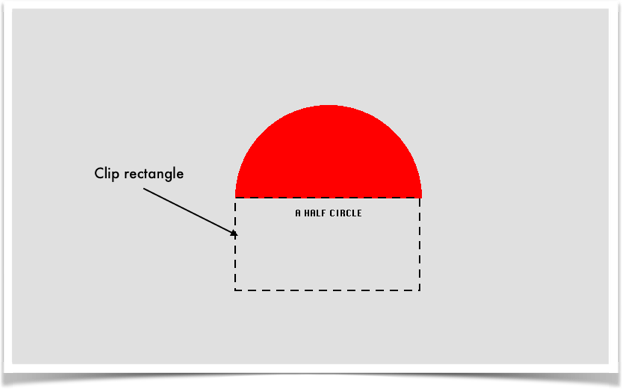
\includegraphics[scale=0.7]{AWFig8.png} 
   \caption{Region with clipping rectangle}
   \label{fig:8 }
\end{figure}

~\\ There is various operations on regions, which are defined in the methods of the class AWRegion, for example :

\begin{enumerate}
\item Release a region which become empty.
\begin{lstlisting}[language=Arduinonl]
//--- release region, becomes empty
  void release (void) ;
\end{lstlisting}

\item Get characteristics of the region.
\begin{lstlisting}[language=Arduinonl]
  inline bool isEmpty (void) const { return NULL == mPtr ; }
  AWInt rectCount (void) const ;
  AWRect rectAtIndex (const AWInt inIndex) const ;
\end{lstlisting}

\item Do operations such as addition or subtraction of a rectangle to/from the region.
\begin{lstlisting}[language=Arduinonl]
//--- Difference from a rectangle
  void operator -= (const AWRect & inRect) ;

//--- Adding a rectangle
  void operator += (const AWRect & inRect) ;
\end{lstlisting}

\item Intersection with a rectangle.
\begin{lstlisting}[language=Arduinonl]
  AWRegion operator & (const AWRect & inRect) const ;
  bool intersects (const AWRect & inOtherRect) const ;
\end{lstlisting}

\item Intersection of regions.
\begin{lstlisting}[language=Arduinonl]
  AWRegion operator & (const AWRegion & inRect) const ;
\end{lstlisting}

\item Enclosing rectangle.
\begin{lstlisting}[language=Arduinonl]
  AWRect enclosingRect (void) const ;
\end{lstlisting}

\item Testing if a point is inside a region.
\begin{lstlisting}[language=Arduinonl]
  bool containsPoint (const AWPoint & inPoint) const ;
  bool containsPoint (const AWInt inX, const AWInt inY) const ;
\end{lstlisting}

\item Handle a copy.
\begin{lstlisting}[language=Arduinonl]
  AWRegion (const AWRegion & inRegion) ;
  AWRegion & operator = (const AWRegion & inRegion) ;
\end{lstlisting}

\end{enumerate}



%%%%%%%%%%%%%%%%%%%%%%%%%%%%%%%%%%%%%%%%%%%%%%
\newpage
\subsection{Colors}

~\\ The AWColor class is not derived from an AWView class.

~\\ A color is defined by 3 bytes (uint\_8) and a boolean. The 3 bytes define respectively the red, green and blue component and the boolean "IsOpaque" define if the color is opaque or transparent.

\begin{lstlisting}[language=Arduinonl]
class AWColor {
//--- Default constructor (clear color)
  inline AWColor (void) : mRed (0), mGreen (0), mBlue (0), mIsOpaque (false) {}

//--- Constructor (custom color)
  inline AWColor (const uint8_t inRed,
                           const uint8_t inGreen,
                           const uint8_t inBlue) :
  mRed (inRed),
  mGreen (inGreen),
  mBlue (inBlue),
  mIsOpaque (true) {
  }
\end{lstlisting}

~\\ A set of 17 colors is predefined to simplify your programming.

\begin{lstlisting}[language=Arduinonl]
  inline static AWColor black (void) {
    return AWColor (0, 0, 0) ;
  }
  inline static AWColor gray (void) {
    return AWColor (128, 128, 128) ;
  }
  inline static AWColor darkGray (void) {
    return AWColor (64, 64, 64) ;
  }
  inline static AWColor lightGray (void) {
    return AWColor (192, 192, 192) ;
  } 
  inline static AWColor veryLightGray (void) {
    return AWColor (224, 224, 224) ;
  } 
  inline static AWColor red (void) {
    return AWColor (255, 0, 0) ;
  }
  inline static AWColor green (void) {
    return AWColor (0, 255, 0) ;
  }
  inline static AWColor blue (void) {
    return AWColor (0, 0, 255) ;
  }
  inline static AWColor white (void) {
    return AWColor (255, 255, 255) ;
  }
  inline static AWColor yellow (void) {
    return AWColor (255, 255, 0) ;
  }
  inline static AWColor orange (void) {
    return AWColor (255, 127, 0) ;
  }
  inline static AWColor brown (void) {
    return AWColor (153, 102, 51) ;
  }
  inline static AWColor cyan (void) {
    return AWColor (0, 255, 255) ;
  }
  inline static AWColor magenta (void) {
    return AWColor (255, 0, 255) ;
  }
  inline static AWColor purple (void) {
    return AWColor (127, 0, 127) ;
  }
  inline static AWColor deepSkyBlue (void) {
    return AWColor (0, 0xBF, 255) ;
  }
  inline static AWColor lightSkyBlue (void) {
    return AWColor (0x87, 0xCE, 0xFA) ;
  }
\end{lstlisting}

~\\ You can set colors, test colors or get colors.

\begin{lstlisting}[language=Arduinonl]
  bool operator == (const AWColor & inOtherColor) const ;
  inline bool operator != (const AWColor & inOtherColor) const {
    return !(*this == inOtherColor) ;
  }
  inline uint8_t redComponent (void) const { return mRed ; }
  inline uint8_t greenComponent (void) const { return mGreen ; }
  inline uint8_t blueComponent (void) const { return mBlue ; }
  inline bool isOpaque (void) const { return mIsOpaque ; }
} ;
\end{lstlisting}


~\\ In the previous example, the red color of the half circle is set by the instruction line :

\begin{lstlisting}[language=Arduinonl]
  AWContext::setColor (AWColor::red ());
\end{lstlisting}

~\\ And generally, you will find a function to set the color in every classes of the \emph{ArduinoWidgets} library.


%%%%%%%%%%%%%%%%%%%%%%%%%%%%%%%%%%%%%%%%%%%%%%
\newpage
\subsection{Fonts}

~\\ The AWFont class is not derived from an AWView class.
~\\ A font is not a View.

~\\ The class AWFont contain font description and fonctions.

\begin{lstlisting}[language=Arduinonl]
class AWFont {
//--- Default constructor: empty font
   AWFont (void) : mFont () {}

//--- Constructor from a font description
  AWFont (const AWFontInternalDefinition & definition) ;

  void drawStringInRegion (const AWInt inX,
                                    const AWInt inY,
                                    const char * inCString,
                                    const AWRegion & inDrawRegion) const ;

  void drawStringInRegion (const AWInt inX,
                                    const AWInt inY,
                                    const String & inString,
                                    const AWRegion & inDrawRegion) const ;

  AWInt ascent (void) const ;
  AWInt descent (void) const ;
  AWInt lineHeight (void) const ;

  AWInt advancement (const uint32_t inCodePoint) const ;

  AWRect stringRect (const AWInt inX,
                              const AWInt inY,
                              const char * inCString) const ;

  AWInt stringLength (const char * inCString) const ;
  AWInt stringLength (const String & inString) const ;


//--- Equatable
  inline bool operator == (const AWFont & inFont) const { return mFont == inFont.mFont ; }
  inline bool operator != (const AWFont & inFont) const { return !(*this == inFont) ; }
} ;
\end{lstlisting}

~\\ The definition of type AWFontInternalDefinition refer to one of these fonts which are already implemented in the \emph{ArduinoWidgets} library :

\begin{lstlisting}[language=Arduinonl]
AWFont-ChicagoDigit-36.h
extern const AWFontInternalDefinition ChicagoDigit36 ;

AWFont-ChicagoFLF12.h
extern const AWFontInternalDefinition ChicagoFLF12 ;

AWFont-ChicagoFLF24.h
extern const AWFontInternalDefinition ChicagoFLF24 ;

AWFont-Geneva10.h
extern const AWFontInternalDefinition Geneva10 ;

AWFont-Geneva12.h
extern const AWFontInternalDefinition Geneva12 ;

AWFont-Geneva9.h
extern const AWFontInternalDefinition Geneva9 ;

AWFont-Lucida_Grande18.h
extern const AWFontInternalDefinition Lucida_Grande18 ;

AWFont-Lucida_Grande24.h
extern const AWFontInternalDefinition Lucida_Grande24 ;
\end{lstlisting}

~\\ These are examples of all fonts :
\begin{figure}[htbp]
   \centering
   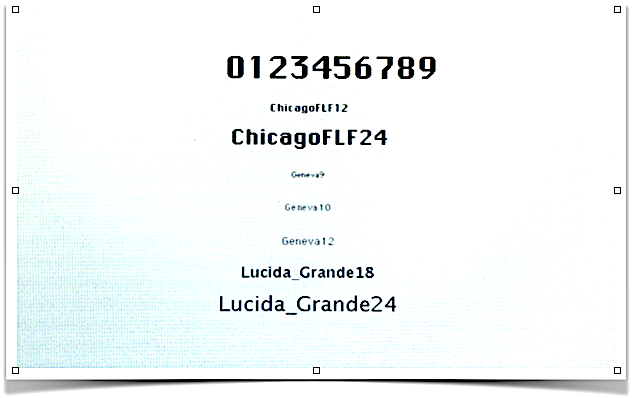
\includegraphics[scale=0.55]{AWFig91.png} 
   \caption{Fonts}
   \label{fig:91 }
\end{figure}


%%%%%%%%%%%%%%%%%%%%%%%%%%%%%%%%%%%%%%%%%%%%%%
\newpage
\section{The existing Views of \emph{ArduinoWidgets}}

~\\ This section describe the View subclasses which are already present in the \emph{ArduinoWidgets} library, that you can use very simply.
~\\ For each View, the class declaration, which is in the .h file of the library, is reproduced without the private properties and methods.
~\\ As explained before, the \texttt{drawInRegion} method is "virtual" and must be defined in the instance of the view in your program.

%%%%%%%%%%%%%%%%
\subsection{Lines}

~\\ A \texttt{AWLine} class inherit from a \texttt{AWView} class. Its constructor is :

\begin{lstlisting}[language=Arduinonl]
  AWLine (const AWPoint & inRelativePoint1,
                   const AWPoint & inRelativePoint2) ;
\end{lstlisting}

~\\ The \texttt{AWLine} class contain the following methods which can be used in your program :

\begin{lstlisting}[language=Arduinonl]
//--- Draw
  virtual void drawInRegion (const AWRegion & inDrawRegion) const ;

//--- Tell the view is opaque
  virtual bool isOpaque (void) const { return false ; }
  };
 \end{lstlisting}

~\\ A line is defined by 2 AWPoints. 
~\\ To create and draw a new line "myLine" from Point1 (50,50) and Point2 (400,400):

\begin{lstlisting}[language=Arduinonl]
//--- Constructor
  AWLine (const AWPoint & inRelativePoint1,
                   const AWPoint & inRelativePoint2) ;
 \end{lstlisting}

~\\ This example display a line from 100,100 to 300,300

\begin{lstlisting}[language=Arduinonl]
AWLine * myLine;
  myLine = new AWLine (AWPoint(100,100), AWPoint(300,300)); 
  addView (myLine) ;
 \end{lstlisting}
~\\ Note that, in this case, you cannot use the origin and destination points for further operations because they are only arguments of the constructor of myLine.

\begin{figure}[htbp]
   \centering
   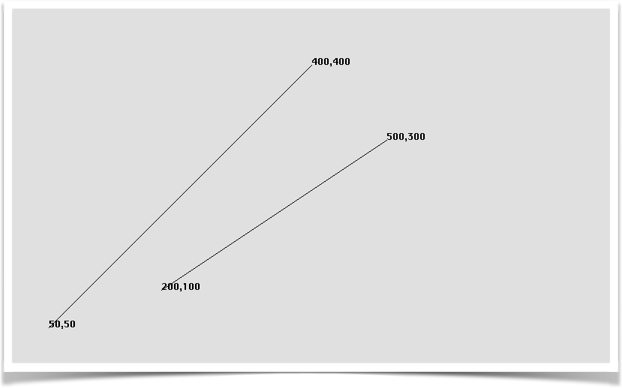
\includegraphics[scale=0.7]{AWFig4.png} 
   \caption{Points and Pixels}
   \label{fig:4 }
\end{figure}

  ~\\ This example display a line from AWPoint lineOrigin(50,50) to AWPoint lineEnd(400,400).

\begin{lstlisting}[language=Arduinonl]
//--- create a black line
  AWPoint lineOrigin ;
  lineOrigin.x = 50 ;
  lineOrigin.y = 50 ;
  AWPoint lineEnd;
  lineEnd.x = 400 ;
  lineEnd.y = 400 ;
  AWLine * myLine1;
  myLine1 = new AWLine (lineOrigin, lineEnd); 
  addView (myLine1) ;
 \end{lstlisting}
~\\ Note that in this case you can use the lineOrigin and lineEnd points for further operations because they are declared outside the constructor of myLine1.

~\\ Note also that AWLine arguments are references (pointers) to AWPoints.

~\\ Note also that pixels are centered on points and, consequently, lines are centered on a grid line.

\begin{figure}[htbp]
   \centering
   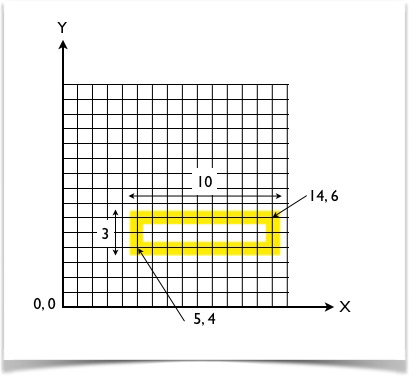
\includegraphics[scale=0.7]{AWFig5.png} 
   \caption{Lines and Pixels}
   \label{fig:5 }
\end{figure}

~\\ Figure 9 show that the dimensions of a line is one pixel more than the width or height used in the drawing method, as it is explained in subsection 5.6.

%%%%%%%%%%%%%%
\newpage
\subsection{Label and AutoLabel}

~\\ A \texttt{Label} is a string of text, "Title", that can be displayed anywhere on the screen (Context) or on a View or subView, or Region
~\\ You can choose a Point and a width to define where the \texttt{Label} is displayed (if the size of the \texttt{Label} is greater than the size, the \texttt{Label} will be clipped. You can choose the alignment of the text with this enum :

\begin{lstlisting}[language=Arduinonl]
typedef enum {
  kAWAlignmentLeft,
  kAWAlignmentCenter,
  kAWAlignmentRight
} AWAlignment ;
\end{lstlisting}

~\\ You can choose the style : the Font and size, the Color 
~\\ The Font and size is choosen from this list :
\begin{itemize}
\item ChicagoDigit36
\item ChicagoFLF12
\item ChicagoFLF24
\item Geneva10
\item Geneva12
\item Geneva9
\item LucidaGrande18
\item LucidaGrande24
\end{itemize}

~\\ You can choose the color from this list : \texttt{black}, \texttt{gray}, \texttt{darkGray}, \texttt{lightGray}, \texttt{veryLightGray}, \texttt{red}, \texttt{green}, \texttt{blue}, \texttt{white}, \texttt{yellow}, \texttt{orange}, \texttt{brown}, \texttt{cyan}, \texttt{magenta}, \texttt{purple}, \texttt{deepSkyBlue}, \texttt{lightSkyBlue}.

~\\ or any other color according to the "Color" section 6.

~\\ Figure 10 show how it is simple to display a Label with these 2 lines of code in the setup():

\begin{lstlisting}[language=Arduinonl]
  addView (new AWLabel(AWPoint ( 300, 250), AWInt (250), AWAlignment (kAWAlignmentCenter), String ("ChicagoFLF24"), AWFont (ChicagoFLF24))) ;
\end{lstlisting}

~\\ or :

\begin{lstlisting}[language=Arduinonl]
  myLabel = new AWLabel(AWPoint ( 300, 340), AWInt (150), AWAlignment (kAWAlignmentCenter), String ("My Label : "), AWFont (Lucida_Grande24)) ;
  addView (myLabel) ;
\end{lstlisting}

~\\ or :

\begin{lstlisting}[language=Arduinonl]
 static AWLabel *gLabel1;
 //--- then in setuo()
  gLabel1 = new AWLabel(AWPoint ( 300, 340), AWInt (150), AWAlignment (kAWAlignmentCenter), String ("My Label : "), AWFont (Lucida_Grande24)) ;
  gLabel1->setBackColor (AWColor::gray() ):
  gLabel1->setTextColor (AWColor::red() ):
  addView (gLabel1) ;
\end{lstlisting}

~\\ The constructor of \texttt{AWLabel} is :

\begin{lstlisting}[language=Arduinonl]
  AWLabel (const AWPoint & inRelativeOrigin,
                    const AWInt inWidth,
                    const AWAlignment inAlignment,
                    const String & inTitle,
                    const AWFont & inFont = awkDefaultFont) ;
\end{lstlisting}

~\\ The AWLabel class contain the following methods which can be used in your program :

\begin{lstlisting}[language=Arduinonl]
//----------- Draw
  virtual void drawInRegion (const AWRegion & inDrawRegion) const ;

//------------ Title
  void setTitle (const String & inTitle) ;
  String title (void) const { return mTitle; }

//------------ Text color
  void setTextColor (const AWColor & inColor) ;

//---------------- Font
  inline AWFont font (void) const { return mFont ; }

//------------ Alignment
  inline AWAlignment alignment (void) const { return mAlignment ; }
  void setAlignment (const AWAlignment inAlignment) ;
\end{lstlisting}

\begin{figure}[htbp]
   \centering
   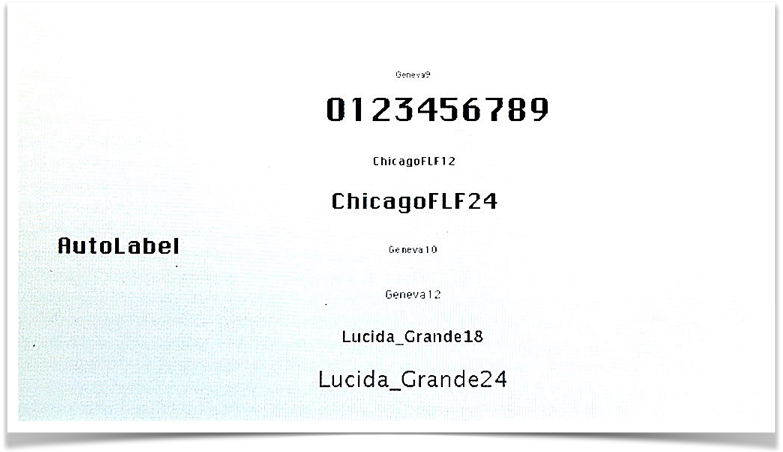
\includegraphics[scale=0.7]{AWFig9.png} 
   \caption{Labels and AutoLabel}
   \label{fig: 9}
\end{figure}


~\\ An \texttt{AutoLabel} is a simplified version of \texttt{Label}, without alignment and width, which are calculated to match automatically the string's size :

\begin{lstlisting}[language=Arduinonl]
class AWAutoLabel : public AWView {
//--- Constructor
  AWAutoLabel (const AWPoint & inRelativeOrigin,
                        const String & inTitle,
                        const AWFont & inFont = awkDefaultFont) ;

//--- Draw
  virtual void drawInRegion (const AWRegion & inDrawRegion) const ;

//------------ Title
  void setTitle (const String & inTitle) ;

//------------ Text color
  void setTextColor (const AWColor & inColor) ;

//---------------- Font
  inline AWFont font (void) const { return mTextFont ; }
} ;
\end{lstlisting}

~\\ The code in the setup() for the Figure 10 is :

\begin{lstlisting}[language=Arduinonl]
  addView (new AWLabel(AWPoint ( 300, 50), AWInt (250), AWAlignment (kAWAlignmentCenter), String ("Lucida_Grande24"), AWFont (Lucida_Grande24))) ;
  addView (new AWLabel(AWPoint ( 300, 100), AWInt (250), AWAlignment (kAWAlignmentCenter), String ("Lucida_Grande18"), AWFont (Lucida_Grande18))) ;
  addView (new AWLabel(AWPoint ( 300, 150), AWInt (250), AWAlignment (kAWAlignmentCenter), String ("Geneva12"), AWFont (Geneva12))) ;
  addView (new AWLabel(AWPoint ( 300, 200), AWInt (250), AWAlignment (kAWAlignmentCenter), String ("Geneva10"), AWFont (Geneva10))) ;
  addView (new AWLabel(AWPoint ( 300, 250), AWInt (250), AWAlignment (kAWAlignmentCenter), String ("ChicagoFLF24"), AWFont (ChicagoFLF24))) ;
  addView (new AWLabel(AWPoint ( 300, 300), AWInt (250), AWAlignment (kAWAlignmentCenter), String ("ChicagoFLF12"), AWFont (ChicagoFLF12))) ;
  addView (new AWLabel(AWPoint ( 300, 350), AWInt (300), AWAlignment (kAWAlignmentCenter), String ("0123456789"), AWFont (ChicagoDigit36))) ;
  addView (new AWLabel(AWPoint ( 300, 400), AWInt (250), AWAlignment (kAWAlignmentCenter), String ("Geneva9"), AWFont (Geneva9))) ;
  addView (new AWAutoLabel(AWPoint ( 50, 200), String ("AutoLabel"), AWFont (ChicagoFLF24))) ;
\end{lstlisting}

~\\ A Label or AutoLabel can be a stand alone view as explained above, or it can be a subview of another view.

~\\ You can change the Title of a Label or AutoLabel as in this exemple to display the freeRam in myLabel :

\begin{lstlisting}[language=Arduinonl]
const size_t gFreeRam = freeRAM () ;
  myLabel->setTitle ("Free Ram: " + String (gFreeRam)) ;
 \end{lstlisting}

~\\ You can display or hide a Label or AutoLabel by changing its visibility :

\begin{lstlisting}[language=Arduinonl]
  myLabel->setVisibility (true) ; // or false
 \end{lstlisting}


%%%%%%%%%%%%%%
\newpage
\subsection{PushButton}

~\\ A \texttt{PushButton} class inherit from a \texttt{AWView} class with an Action. The View is a roundRectangle with a title inside.
~\\ When the user click inside the Button, an action is sent to a receiver.

~\\ The PushButton class contain the following constructors :

\begin{lstlisting}[language=Arduinonl]
  AWPushButton (const AWPoint & inRelativeBaselineOrigin,
                         const AWInt inWidth,
                         const String & inTitle,
                         const AWFont & inFont = awkDefaultFont) ;
  
  AWPushButton (const AWRect & inFrame,
                         const String & inTitle,
                         const AWFont & inFont = awkDefaultFont) ;
\end{lstlisting}

~\\ The example below show a unique PushButton centered in the screen with a number inside. Each time you click in the button, the number inside the button is incremented.

~\\ The code of this example include a declaration before the setup() :

\begin{lstlisting}[language=Arduinonl]
//--- Current button value
int buttonValue = 0 ;

//--- button action
void bigButtonAction (AWView * inSender)
{
  AWPushButton * sendingButton = (AWPushButton *) inSender ;
  buttonValue ++ ;
  sendingButton->setTitle (String (buttonValue)) ;
}
\end{lstlisting}

~\\ and an initialization of the button in the setup() :

\begin{lstlisting}[language=Arduinonl]
 // create a big button centered on screen
  AWPushButton * bigButton = new AWPushButton(AWRect (0, 0, 300, 100), String (buttonValue), AWFont (ChicagoDigit36)) ;
  bigButton->setAction (bigButtonAction) ;
  addCenteredView (bigButton) ;
\end{lstlisting}

\begin{figure}[htbp]
   \centering
   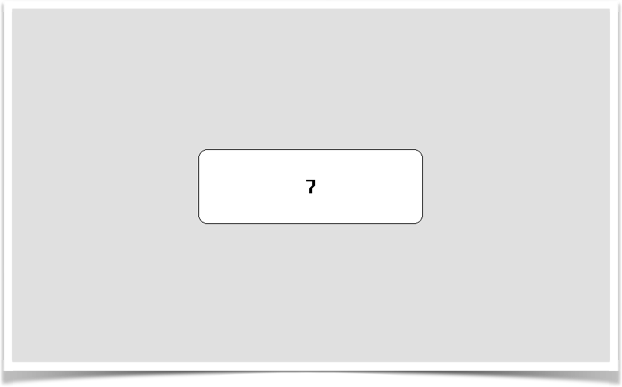
\includegraphics[scale=0.7]{AWFig10.png} 
   \caption{A PushButton}
   \label{fig: 10}
\end{figure}

~\\ The receiver of the PushButton is the Title of the button itself, but, in general, it can be any receiver inside any other object View.

~\\ The bigButtonAction function is activated each time there is a click in this button. It execute what you want to do.
  
~\\ The PushButton class contain the following methods which can be used in your program :

\begin{lstlisting}[language=Arduinonl]
//------------ Title
  protected : String mTitle ;
  void setTitle (const String & inTitle) ;
//---------------- Font
  inline AWFont font (void) const { return mFont ; }
//--- Draw
  virtual void drawInRegion (const AWRegion & inDrawRegion) const ;
//--- Properties
  inline AWColor textColor (void) const { return mTextColor ; }
  void setTextColor (const AWColor inTextColor) { mTextColor = inTextColor ; }  
  protected : AWInt mStringDisplayLength ;
  inline AWInt verticalMargin (void) const { return mVerticalMargin ; }
//--- Enabled state
  inline bool isEnabled (void) const { return mIsEnabled ; }
  void setEnabled (const bool inState) ;
//--- Hilite state
  inline bool isHilited (void) const { return mHiliteState ; }
//--- Tell the view is opaque or not
  virtual bool isOpaque (void) const ;
//--- Touch
  virtual void touchDown (const AWPoint & inPoint) ;
  virtual void touchMove (const AWPoint & inPoint) ;
  virtual void touchUp (const AWPoint & inPoint) ;
} ;
\end{lstlisting}

~\\ This example show a View with 4 PushButtons as subVievs. It implements also the actions which are done when clicking in a button.

~\\ In the declaration part, we create a base View which will contain the PushButtons and the actions on this View :
\begin{lstlisting}[language=Arduinonl]
static AWView * gBaseView ;
// This base View will move 20 pixels when clicking in a button
// We declare the respective actions which will apply : a translation
static void leftButtonAction (AWView * inSender) {
  gBaseView->translateBy (-20, 0) ;
}
static void rightButtonAction (AWView * inSender) {
  gBaseView->translateBy (20, 0) ;
}
static void upButtonAction (AWView * inSender) {
  gBaseView->translateBy (0, 20) ;
}
static void downButtonAction (AWView * inSender) {
  gBaseView->translateBy (0, -20) ;
}\end{lstlisting}

~\\ In the setup(), we put everything in place :
\begin{lstlisting}[language=Arduinonl]
  gBaseView = new AWView (AWRect (550, 150, 140, 95), awkBackColor) ;
  addView (gBaseView) ;
  view = new AWPushButton (AWPoint (5, 40), 60, "Left") ;
  view->setAction (leftButtonAction) ;
  gBaseView->addSubView (view) ;
  view = new AWPushButton (AWPoint (75, 40), 60, "Right") ;
  view->setAction (rightButtonAction) ;
  gBaseView->addSubView (view) ;
  view = new AWPushButton (AWPoint (40, 15), 60, "Down") ;
  view->setAction (downButtonAction) ;
  gBaseView->addSubView (view) ;
  view = new AWPushButton (AWPoint (40, 70), 60, "Up") ;
  view->setAction (upButtonAction) ;
  gBaseView->addSubView (view) ;
\end{lstlisting}

~\\ Everything is done by \texttt{AWContext::handleTouchAndDisplay ()} in the \texttt{loop}.
~\\ This figure show the 4 PushButtons. Left, the base View is not visible (awkBackColor) and right, the base View is visible (gray).

\begin{figure}[htbp]
   \centering
   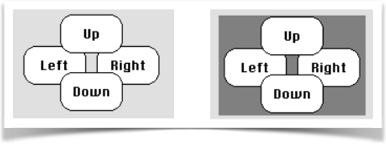
\includegraphics[scale=0.7]{AWFig101.png} 
   \caption{A view with 4 PushButton subviews}
   \label{fig:101}
\end{figure}


~\\There will be further examples of PushButton together with examples of other views.

%%%%%%%%%%%%%%
\newpage
\subsection{SegmentedControl}

~\\ A \texttt{SegmentedControl} class inherit from a \texttt{AWView} class, with an Action.
~\\ For example, this series of 3 tabs which divide a SegmentedControl view in 3 actions
~\\

\begin{figure}[htbp]
   \centering
   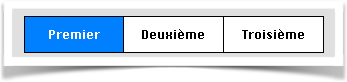
\includegraphics[scale=0.7]{AWFig11.png} 
   \caption{SegmentedControl}
   \label{fig:11}
\end{figure}

~\\

~\\ The SegmentedControl class contain the following constructor :

\begin{lstlisting}[language=Arduinonl]
  AWSegmentedControl (const AWPoint & inRelativeBaselineOrigin,
                               const AWInt inWidth,
                               const AWFont & inFont = awkDefaultFont) ;
\end{lstlisting}

~\\ The SegmentedControl class contain the following methods which can be used in your program :

\begin{lstlisting}[language=Arduinonl]
//--- Draw
  virtual void drawInRegion (const AWRegion & inDrawRegion) const ;

//--- Adding a Tab
  void addTab (const String & inTitle) ;

//--- Utilities
  AWRect tabTitleRectForIndex (const AWInt inIndex) const ;

//---------------- Font
  inline AWFont font (void) const { return mFont ; }

//--- Properties
  inline AWInt selectedTabIndex (void) const { return mSelectedTabIndex ; }
  void selectTabAtIndex (const AWInt inIndex) ;

//---------------- Segmented control action
typedef void (* AWSegmentedControlAction) (AWSegmentedControl * inSender, const AWInt inHilitedTabIndex) ;

// If segmented control action is NULL (by default), touch up changes selection and send action (defined in AWView)
// If not NULL, touch up does not change selection, and sends segmented control action
  inline AWSegmentedControlAction segmentedControlAction (void) const { return mSegmentedControlAction ; }
  inline void setSegmentedControlAction (const AWSegmentedControlAction inAction) {
    mSegmentedControlAction = inAction ;
  }

//---------------- Touch
  virtual void touchDown (const AWPoint & inPoint) ;
  virtual void touchMove (const AWPoint & inPoint) ;
  virtual void touchUp (const AWPoint & inPoint) ;

//---------------- Enabled state
  inline bool isEnabled (void) const { return mIsEnabled ; }
  void setEnabled (const bool inState) ;
} ;
\end{lstlisting}

~\\ The exemple of Figure 13 have, in the declaration part :

\begin{lstlisting}[language=Arduinonl]
  static AWSegmentedControl * gSegmentedControl ;
  
  static void segmentedControlAction (AWSegmentedControl * inSender, const AWInt inHilitedTabIndex) {
    beep () ;
    digitalWrite(LED_BUILTIN, !digitalRead(LED_BUILTIN));
}
\end{lstlisting}

~\\ Then in the setup part :

\begin{lstlisting}[language=Arduinonl]
  gSegmentedControl = new AWSegmentedControl (AWPoint (440, 100), 300) ;
  gSegmentedControl->addTab ("Premier") ;
  gSegmentedControl->addTab ("Deuxieme") ;
  gSegmentedControl->addTab ("Troisieme") ;
  //  gSegmentedControl->setEnabled (false) ;
  gSegmentedControl->setSegmentedControlAction (segmentedControlAction) ;
  addView (gSegmentedControl) ;
\end{lstlisting}

~\\ This example sound a beep and turn the built-in led on or off when clicking in any of the tabs.



%%%%%%%%%%%%%%
\newpage
\subsection{Slider}

~\\ A \texttt{Slider} class inherit from a \texttt{AWView} class with an Action.
~\\ A Slider is a complex View class which can control any entity by simply moving a cursor along a linear potentiometer.
~\\ When the slider is moved (translated) an action is sent to a receiver with the value of the slider.

~\\ The Slider class contain the following constructor :

\begin{lstlisting}[language=Arduinonl]
const bool kHorizontal = false;
const bool kVertical = true;

  AWSlider (const AWPoint & inOrigin,
                     const AWInt inSize,
                     const bool inOrientation,
                     const bool inHasRuler = true) ;
\end{lstlisting}

~\\ In this example, one slider control the brightness of the backlight of the screen, and the 3 other sliders control the color of a colorView (a simple rectangle).

\begin{figure}[htbp]
   \centering
   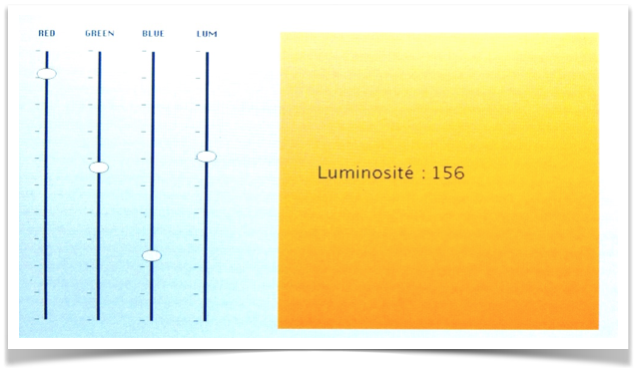
\includegraphics[scale=0.7]{AWFig12.png} 
   \caption{Four Sliders to control the brightness and the color of a Rectangle}
   \label{fig:12 }
\end{figure}

~\\ This exemple include a declaration part before the setup() :

\begin{lstlisting}[language=Arduinonl]
//--- Label
AWLabel * label1;
AWLabel * label2;

//--- Current color value
AWColor displayedColor = AWColor::white () ;

AWSlider *redSlider;
AWSlider *greenSlider;
AWSlider *blueSlider;
AWSlider *backlightSlider;
AWView *colorView;

//--- Slider action
void sliderAction (AWView * inSender)
{
  AWSlider * sendingSlider = (AWSlider *) inSender ;
  AWInt pos = sendingSlider->knobPosition ();
  if (sendingSlider == backlightSlider) {
    analogWrite (BACKLIGHT, pos);
    label2->setTitle(pos);
  }
  else {
    AWColor newColor(redSlider->knobPosition (), greenSlider->knobPosition (), blueSlider->knobPosition ());
    colorView->setBackColor (newColor) ;
  }
  \end{lstlisting}

~\\ and an initialization of the sliders and receivers in the setup() :

\begin{lstlisting}[language=Arduinonl]
 redSlider = new AWSlider (AWPoint (30,30), 400, kVertical, true) ;
  redSlider->setMaxKnobPosition (255);
  redSlider->setKnobPosition (255);
  redSlider->setAction (sliderAction);
  addView (redSlider) ;
  addView (new AWLabel (AWPoint (25, 440), 40, kAWAlignmentCenter, "RED")) ;
  
  greenSlider = new AWSlider (AWPoint (100,30), 400, kVertical, true) ;
  greenSlider->setMaxKnobPosition (255);
  greenSlider->setKnobPosition (255);
  greenSlider->setAction (sliderAction);
  addView (new AWLabel (AWPoint (95, 440), 40, kAWAlignmentCenter, "GREEN")) ;

  blueSlider = new AWSlider (AWPoint (170,30), 400, kVertical, true) ;
  blueSlider->setMaxKnobPosition (255);
  blueSlider->setKnobPosition (255);
  blueSlider->setAction (sliderAction);
  addView (new AWLabel (AWPoint (165, 440), 40, kAWAlignmentCenter, "BLUE")) ;

  backlightSlider = new AWSlider (AWPoint (240,30), 400, kVertical, true) ;
  backlightSlider->setMaxKnobPosition (255);
  backlightSlider->setKnobPosition (200);
  backlightSlider->setAction (sliderAction);
  addView (new AWLabel (AWPoint (235, 440), 40, kAWAlignmentCenter, "LUM")) ;

  addView (greenSlider) ;
  addView (blueSlider) ;
  addView (backlightSlider) ;
  colorView = new AWView (AWRect (350, 30, 420, 420), AWColor::white());
  addView (colorView) ;

  label1 = new AWLabel(AWPoint ( 400, 240), AWInt (150), AWAlignment (kAWAlignmentLeft), String ("Brightness : "), AWFont (Lucida\_Grande24)) ;
  addView (label1) ;
  label2 = new AWLabel(AWPoint ( 550, 240), AWInt (100), AWAlignment (kAWAlignmentLeft), String ("200"), AWFont (Lucida_Grande24)) ;
  addView (label2) ;
\end{lstlisting}


~\\ The Slider class contain the following methods which can be used in your program :

\begin{lstlisting}[language=Arduinonl]
  //--- Draw
  virtual void drawInRegion ( const AWRegion & inDrawRegion ) const ;
   
  //--- Orientation
  bool orientation() const { return mOrientation ; }
  
  //--- Knob color
  protected : AWColor mKnobColor ;
  
  //--- Ruler display
  protected : void drawRulerInRegion ( const AWRegion & inDrawRegion ) const ;
  bool hasRuler() const { return mHasRuler ; }
  //--- Set the number of scales on the slider. Any value < 1 sets mHasRuler
  //--- to false so that no ruler is displayed
  void setHowManyScales ( const AWInt inHowManyScales ) ;
  
  //--- Position
  inline AWInt knobPosition (void) const { return mKnobPosition ; }
  void setKnobPosition ( AWInt inKnobPosition, const bool inRefresh = false ) ;
  inline AWInt maxKnobPosition (void) const { return mMaxKnobPosition ; }
  void setMaxKnobPosition ( AWInt inMaxKnobPosition ) ;
  protected : AWRect knobRect() const ;
  
  //--- Enabled state
  inline bool isEnabled (void) const { return mIsEnabled ; }
//  void setEnabled (const bool inState) ;
  
  //--- Tell the view is opaque or not
  virtual bool isOpaque (void) const ;
  
  //--- Touch
  virtual void touchDown (const AWPoint & inPoint) ;
  virtual void touchMove (const AWPoint & inPoint) ;
  virtual void touchUp (const AWPoint & inPoint) ;
\end{lstlisting}

~\\ This example show one horizontal slider and one vertical slider, both having division scales. Both sliders are combined with a respective AutoLabel to display their position.

\begin{figure}[htbp]
   \centering
   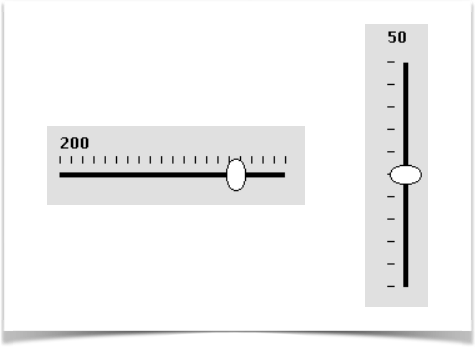
\includegraphics[scale=0.7]{AWFig121.png} 
   \caption{Sliders with scales lines}
   \label{fig:121 }
\end{figure}

~\\ The declarations are :

\begin{lstlisting}[language=Arduinonl]
static AWSlider * gSliderH;
static AWSlider * gSliderV;
static AWAutoLabel * gSliderHLabel;
static AWAutoLabel * gSliderVLabel;
\end{lstlisting}

~\\ The actions are :

\begin{lstlisting}[language=Arduinonl]
static void updateHSliderLabelAction (AWView * inSender)
{
  AWSlider * sendingSlider = (AWSlider *) inSender ;
  AWInt pos = sendingSlider->knobPosition ();
  if (sendingSlider == gSliderH) {
    gSliderHLabel->setTitle(pos);
  }
}
static void updateVSliderLabelAction (AWView * inSender)
{
  gSliderVLabel->setTitle(String(((AWSlider *)inSender)->knobPosition()));
}
\end{lstlisting}

~\\ The setup, with \texttt{setHowManyScales} and combined labels is :

\begin{lstlisting}[language=Arduinonl]
  gSliderH = new AWSlider(AWPoint(300,200),200,kHorizontal) ;
  gSliderH->setHowManyScales( 20 ) ;
  gSliderH->setMaxKnobPosition (255);
  gSliderH->setKnobPosition (200);
  addView(gSliderH) ;
  gSliderHLabel = new AWAutoLabel ( AWPoint( 310, 235), "200" ) ;
  gSliderH->setAction(updateHSliderLabelAction) ;
  addView(gSliderHLabel);
  
  gSliderV = new AWSlider(AWPoint(725,140),200,kVertical) ;
  addView(gSliderV) ;
  gSliderVLabel = new AWAutoLabel ( AWPoint( 725, 345 ), "50" ) ;
  gSliderV->setAction(updateVSliderLabelAction) ;
  addView(gSliderVLabel) ;
\end{lstlisting}



%%%%%%%%%%%%%%
\newpage
\subsection{DynamicSlider}

~\\ A \texttt{DynamicSlider} class inherit from a \texttt{AWView} class.

~\\ A \texttt{DynamicSlider} is a Slider with 2 knobs. One elliptic \emph{main} knob exactly the same as in a Slider, and one smaller and circular \emph{target} knob which can be hidden when its position is the same as the main knob's position.
~\\ The main knob is movable with the touch control as usual and the dynamic knob can follow the main knob but slowly and smoothly. Both knobs have respective positions, so the dynamic knob can be used to create a smooth evolution os a parameter, such as the sound level in a mixing table or a smooth acceleration of a locomotive.
~\\

\begin{figure}[htbp]
   \centering
   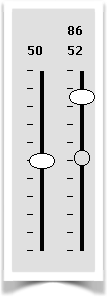
\includegraphics[scale=0.7]{AWFig13.png} 
   \caption{A Slider (left) and a dynamic Slider (right)}
   \label{fig:13}
\end{figure}

~\\

~\\ The DynamicSlider class contain the following constructor and methods

\begin{lstlisting}[language=Arduinonl]
class AWDynamicSlider : public AWSlider
{
  AWDynamicSlider ( const AWPoint & inOrigin,
                             const AWInt inSize,
                             const bool inOrientation,
                             const bool inHasRuler = true ) ;
  
  //--- Draw
  virtual void drawInRegion ( const AWRegion & inDrawRegion ) const ;
  
  //--- Position
  inline AWInt dynamicKnobPosition (void) const { return mDynKnobPosition ; }
  void setDynamicKnobPosition ( AWInt inKnobPosition ) ;
};
\end{lstlisting}

~\\ The example of figure 16 show a vertical dynamic slider, combined with two AutoLabel to display the respective positions of the main and target knobs (right slider only).
~\\

~\\ The declarations are :

\begin{lstlisting}[language=Arduinonl]
static AWDynamicSlider * gDynSliderV;
\end{lstlisting}

~\\ The actions are :

\begin{lstlisting}[language=Arduinonl]
static void updateDynamicVSliderLabelAction (AWView * inSender)
{
  gDynamicSliderVLabelTarget->setTitle(String(((AWDynamicSlider *)inSender)->knobPosition()));
  gDynamicSliderVLabelCurrent->setTitle(String(((AWDynamicSlider *)inSender)->dynamicKnobPosition()));
}
\end{lstlisting}

~\\ The setup, with combined main and target labels is :

\begin{lstlisting}[language=Arduinonl]
  gDynSliderV = new AWDynamicSlider(AWPoint(765,140),200,kVertical) ;
  addView(gDynSliderV) ;
  gDynamicSliderVLabelCurrent = new AWAutoLabel ( AWPoint( 765, 345), "50") ;
  gDynamicSliderVLabelTarget = new AWAutoLabel ( AWPoint( 765, 365), "50") ;
  gDynSliderV->setAction(updateDynamicVSliderLabelAction) ;
  addView(gDynamicSliderVLabelCurrent) ;
  addView(gDynamicSliderVLabelTarget) ;
\end{lstlisting}

~\\ Finally, in order to move automatically the target knob  in order to join slowly the main knob, the following code is added in the loop, with a global \texttt{static unsigned gDynamicDeadLine} which store the system time :

\begin{lstlisting}[language=Arduinonl]
  if (gDynamicDeadLine <= millis()) {
    gDynamicDeadLine += 100;
    AWInt targetPos = gDynSliderV->knobPosition();
    AWInt currentPos = gDynSliderV->dynamicKnobPosition();
    if (currentPos < targetPos) {
      gDynSliderV->setDynamicKnobPosition(currentPos + 1);
    }
    else if (currentPos > targetPos) {
      gDynSliderV->setDynamicKnobPosition(currentPos - 1);
    }
  }
\end{lstlisting}


%%%%%%%%%%%%%%
\newpage
\subsection{TabView}

~\\ A \texttt{TabView} class inherit from a \texttt{AWView} class
~\\ A TabView is a navigation interface. It is a view looking like a tab bar controller to organize your app into one or more distinct modes of operation. The view hierarchy of a tab bar controller is self contained. It is composed of views that the tab bar controller manages directly and views that are managed by content views  you provide. Each content view manages a distinct view hierarchy, and the TabView coordinates the navigation between the view hierarchies.
~\\The key component of a TabView interface is the presence of a tab bar view along the bottom of the screen (for example). This view is used to initiate the navigation between your app’s different modes and can also convey information about the state of each mode.
~\\The TabView creates and manages its own view and also manages the views that provide the content view for each mode.

\begin{figure}[htbp]
   \centering
   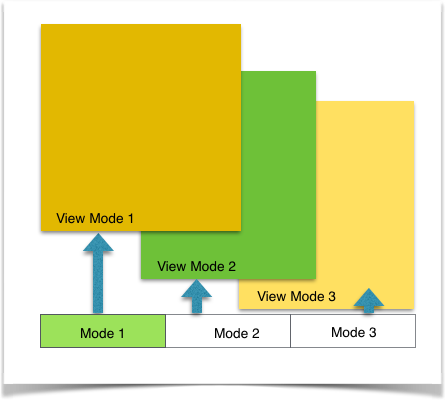
\includegraphics[scale=0.7]{AWFig14.png} 
   \caption{a TavView controlling views}
   \label{fig:14 }
\end{figure}

~\\

~\\ The TabView class contain the following constructor and methods

\begin{lstlisting}[language=Arduinonl]
class AWTabView : public AWView {
//--- Constructor
  AWTabView (const AWRect & inRelativeFrame,
                      const AWFont & inFont = awkDefaultFont) ;

//--- Destructor
  virtual ~ AWTabView (void) ;

//--- Draw
  virtual void drawInRegion (const AWRegion & inDrawRegion) const ;

//--- Adding a Tab
  void addTab (const String & inTitle, AWView * inView) ;

//---------------- Font
  inline AWFont font (void) const { return mFont ; }

//--- Utilities
  AWInt titleHeight (void) const ;
  AWRect horizontalSeparator (void) const ;
  AWRect contentRectFromFrame (const AWRect & inFrame) const ;
  AWRect titleRect (void) const ;
  AWRect tabTitleRectForIndex (const AWInt inIndex) const ;

//--- Properties
  inline AWInt selectedTabIndex (void) const { return mSelectedTabIndex ; }
  void selectTabAtIndex (const AWInt inIndex) ;

//---------------- Badge
  void setBadgeAtIndex (const AWInt inIndex, const bool inDisplayBadge) ; // Does nothing if index if out of mList bounds
  bool hasBadgeAtIndex (const AWInt inIndex) const ; // return false if index if out of mList bounds
  AWRect badgeRect (const AWInt inItemIndex) const ;

//---------------- Touch
  virtual void touchDown (const AWPoint & inPoint) ;
  virtual void touchMove (const AWPoint & inPoint) ;
  virtual void touchUp (const AWPoint & inPoint) ;
} ;
\end{lstlisting}

~\\ An example of TabView is given in the following code :
~\\ First declare a AWTabView : gTabView

\begin{lstlisting}[language=Arduinonl]
static AWTabView * gTabView ;
\end{lstlisting}

~\\ Then, in the setup, create the gTabView and 4 views which are here simple rectangles. Each view is associated with a teb by addTab which define the label in the tab and the associated view. Doing that 4 times create a 4 tab TabView

\begin{lstlisting}[language=Arduinonl]
  gTabView = new AWTabView (AWRect (10, 10, 550, 500)) ;
  AWView * view ;
  view = new AWView (AWRect (0, 0, 250, 300), AWColor::brown ()) ;
  gTabView->addTab ("First", view) ;
  view = new AWView (AWRect (100, 0, 250, 300), AWColor::yellow ()) ;
  gTabView->addTab ("Second", view) ;
  view = new AWView (AWRect (200, 0, 250, 300), AWColor::cyan ()) ;
  gTabView->addTab ("Third", view) ;
  view = new AWView (AWRect (300, 0, 250, 300), AWColor::purple ()) ;
  gTabView->addTab ("Fourth", view) ;
  addView (gTabView) ;
\end{lstlisting}


~\\ And its all !

\begin{figure}[htbp]
   \centering
   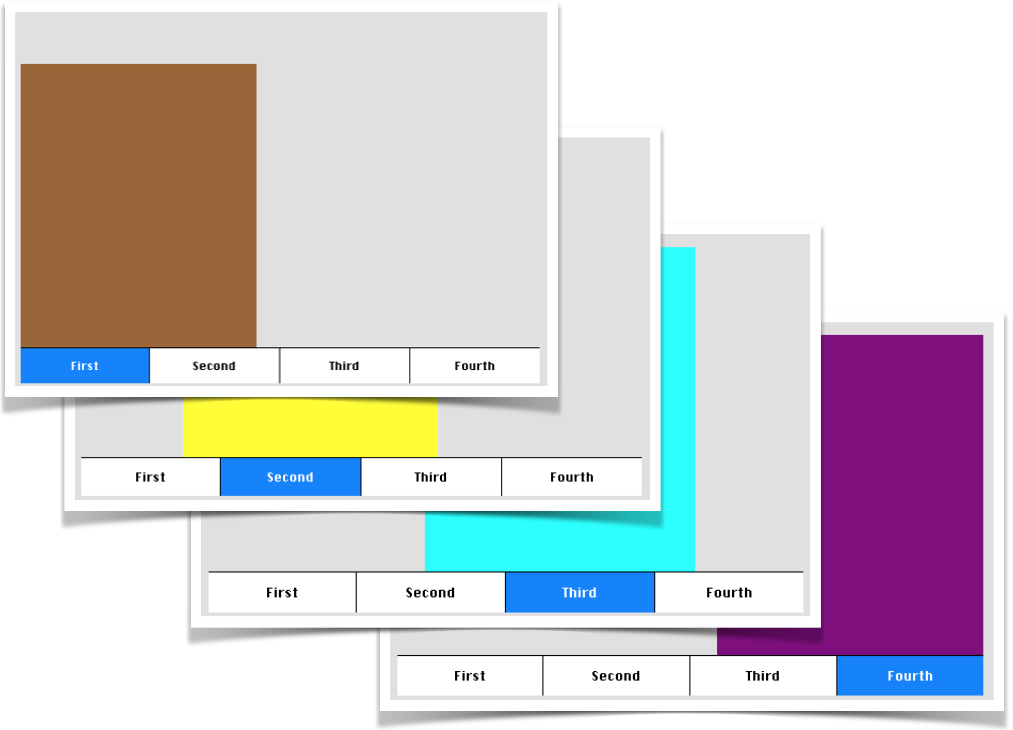
\includegraphics[scale=0.4]{AWFig141.png} 
   \caption{A 4 tabs TabView controlling 4 views}
   \label{fig:14 }
\end{figure}


%%%%%%%%%%%%%%
\newpage
\subsection{Switch}

~\\ A \texttt{Switch} class inherit from a \texttt{AWView} class
~\\ A Switch is like a checkbox which can be toggled between true or false when clicking on it. Switches are commonly used to indicate whether a feature is enabled or disabled. You set the initial value of the switch in your program, but you can modify that value at runtime using the methods of this class.
~\\ A Switch is defined by a Point and a string Title (and a Font if you except the default font).
~\\

\begin{figure}[htbp]
   \centering
   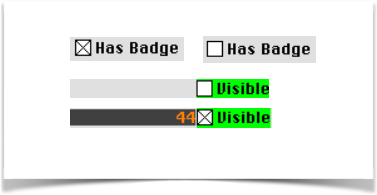
\includegraphics[scale=0.55]{AWFig15.png} 
   \caption{Some Switches}
   \label{fig:15 }
\end{figure}

~\\

~\\ The Switch class contain the following constructor and methods

\begin{lstlisting}[language=Arduinonl]
class AWSwitch : public AWView {
//--- Constructor
  AWSwitch (const AWPoint & inBaseLineRelativeOrigin,
                     const String & inTitle,
                     const AWFont & inFont = awkDefaultFont) ;

//--- Draw
  virtual void drawInRegion (const AWRegion & inDrawRegion) const ;

//---
  void setTitle (const String & inTitle) ;
  AWRect boxRect (void) const ;

//---------------- Font
  inline AWFont font (void) const { return mFont ; }

//------------- State
  inline bool checked (void) const { return mChecked ; }
  void setChecked (const bool inChecked) ;

//---------------- Hilite state
  protected : bool mHiliteState ; // false (by default): not hilited

//--- Enabled state
  inline bool isEnabled (void) const { return mIsEnabled ; }
  void setEnabled (const bool inState) ;

//---------------- Touch
  virtual void touchDown (const AWPoint & inPoint) ;
  virtual void touchMove (const AWPoint & inPoint) ;
  virtual void touchUp (const AWPoint & inPoint) ;
} ;
\end{lstlisting}

~\\ To create the example of the above figure, you declare a gSwitch :

\begin{lstlisting}[language=Arduinonl]
static AWSwitch * gSwitch ;
\end{lstlisting}

~\\ And an action depending of the state of the gSwitch : In this example the action is to change the visibility of a label.

\begin{lstlisting}[language=Arduinonl]
static void switchAction (AWView * inSender) {
  gLabel2->setVisibility (gSwitch->checked ()) ;
}
\end{lstlisting}

~\\ Then, in the setup, create the gSwitch view with the title "Visible" and its associated action. Each time you click in the gSwitch the action will be executed.

\begin{lstlisting}[language=Arduinonl]
  gSwitch = new AWSwitch (AWPoint (102, 95), "Visible") ;
  gSwitch->setBackColor (AWColor::green ()) ;
  gSwitch->setAction (switchAction) ;
  addView (gSwitch) ;
  gSwitch->sendAction () ;
\end{lstlisting}
  
~\\

%%%%%%%%%%%%%%
\newpage
\subsection{ArrowPushButton}

~\\ A \texttt{ArrowPushButton} class inherit from a \texttt{AWView} class
~\\ An \texttt{ArrowPushButton} is a \texttt{PushButton} with an arrow picture inside and no title.
~\\ It is used exactly as a \texttt{PushButton}, but you can choose the direction and color of the arrow.
~\\

\begin{figure}[htbp]
   \centering
   
\includegraphics[scale=0.55]{AWFig16.png} 
   \caption{An ArrowPushButton}
   \label{fig:16 }
\end{figure}

~\\

~\\ The \texttt{ArrowPushButton} class contain the following constructor and methods

\begin{lstlisting}[language=Arduinonl]
enum { kUpArrow, kDownArrow, kRightArrow, kLeftArrow } ;

class AWArrowPushButton : public AWView
{
  public: AWArrowPushButton(const AWRect & inRelativeFrame,
                            const uint32_t inArrowDirection,
                            const AWColor & inArrowColor) ;

  //--- Arrow color
  private: uint32_t mArrowDirection ;
  //--- Arrow color
  private: AWColor mArrowColor ;
  public: AWColor arrowColor() const { return mArrowColor; } ;
  public: void setArrowColor(AWColor & inArrowColor) { mArrowColor = inArrowColor; } ;

  //--- Enabled state
  inline bool isEnabled (void) const { return mIsEnabled ; }
  void setEnabled (const bool inState) ;

  //--- On Off state management
  inline bool isOn() const { return mIsOn ; }
  inline void setIsOn (const bool inIsOn) { mIsOn = inIsOn ; }

  inline bool onOffState() const { return mOnOffState ; }
  inline void setOnOffState(const bool inOnOffState) { mOnOffState  = inOnOffState ; }

  //--- Draw
  virtual void drawInRegion (const AWRegion & inDrawRegion) const ;

  //--- Tell the view is opaque or not
  virtual bool isOpaque (void) const ;

  //--- Touch
  virtual void touchDown (const AWPoint & inPoint) ;
  virtual void touchMove (const AWPoint & inPoint) ;
  virtual void touchUp (const AWPoint & inPoint) ;
};
\end{lstlisting}

~\\ The following code show how to use an \texttt{ArrowPushButton} in the \texttt{setup}. First, button is created with arguments for its coordinates, its direction its color.

\begin{lstlisting}[language=Arduinonl]
AWArrowPushButton * button = new AWArrowPushButton( AWRect(750,0,50,80), kUpArrow, AWColor::blue() ) ;
  button->setAction (showKeyboard) ;
  addView (button) ;
\end{lstlisting}

~\\ Then we set the attached action which is showing a keyboard as described in the next sections. Then there is the traditional \texttt{addview}.

%%%%%%%%%%%%%%
\newpage
\subsection{AWKeyButton}

~\\ A \texttt{AWKeyButton} class inherit from a \texttt{AWView} class
~\\ A AWKeyButton is a unique key button which is a part of a keyboard. The AWKeyboard class is described hereafter.
~\\
~\\

\begin{figure}[htbp]
   \centering
   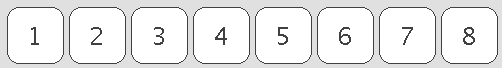
\includegraphics[scale=0.6]{AWFig17.png} 
   \caption{A series of AWKeyButtons}
   \label{fig:17}
\end{figure}

~\\

~\\ The AWKeyButton class contain the following constructor and methods

\begin{lstlisting}[language=Arduinonl]
class AWKeyButton : public AWView
{
  AWKeyButton (const AWRect & inFrame,
                        const AWColor & inBackColor) ;
  
  virtual void setShifted (const bool inShifted,
                                    const AWView * const inSender) ;

  //---------------- Hilite state
  inline bool isHilited (void) const { return mHiliteState; }
  
  //---------------- Drawing
  protected : void drawFrameAndBackgroundInRegion (const AWRegion & inDrawRegion) const ;
  virtual bool isOpaque (void) const ;

  //--- Touch
  virtual void touchDown (const AWPoint & inPoint) ;
  virtual void touchMove (const AWPoint & inPoint) ;
  virtual void touchUp (const AWPoint & inPoint) ;
};
\end{lstlisting}

~\\ The AWKeyButton class have the following derived classes which differ to build a complete set of keybuttons of a full keyboard.

~\\ The AWNormalKeyButton class contain the following constructor and methods

\begin{lstlisting}[language=Arduinonl]
class AWNormalKeyButton : public AWKeyButton
{
  AWNormalKeyButton (const AWRect & inFrame,
                              const char inText,
                              const char inShiftText) ;
  
  virtual void setShifted (const bool inShifted,
                                    const AWView * const inSender) ;
  
  char keyChar () const { return mCurrentKey ; }
  
  //--- Draw
  virtual void drawInRegion (const AWRegion & inDrawRegion) const ;
};
\end{lstlisting}

~\\ The AWReturnKeyButton class contain the following constructor and methods

\begin{lstlisting}[language=Arduinonl]
class AWReturnKeyButton : public AWKeyButton
{
  AWReturnKeyButton (const AWRect & inFrame) ;
  
  //--- Draw
  virtual void drawInRegion (const AWRegion & inDrawRegion) const ;
};
\end{lstlisting}

~\\ The AWBackspaceKeyButton class contain the following constructor and methods

\begin{lstlisting}[language=Arduinonl]
class AWBackspaceKeyButton : public AWKeyButton
{
  AWBackspaceKeyButton (const AWRect & inFrame) ;
  
  //--- Draw
  virtual void drawInRegion (const AWRegion & inDrawRegion) const ;
};
\end{lstlisting}

~\\ The AWShiftKeyButton class contain the following constructor and methods

\begin{lstlisting}[language=Arduinonl]
class AWShiftKeyButton : public AWKeyButton
{
  AWShiftKeyButton (const AWRect & inFrame, const bool inRightAlign) ;
  
  //---- Alignment of the arrow in the key
  virtual void setShifted (const bool inShifted,
                                    const AWView * const inSender) ;
  
  //--- Draw
  virtual void drawInRegion (const AWRegion & inDrawRegion) const ;
};
\end{lstlisting}

~\\ The AWLeftArrowKeyButton class contain the following constructor and methods

\begin{lstlisting}[language=Arduinonl]
class AWLeftArrowKeyButton : public AWKeyButton
{
  AWLeftArrowKeyButton (const AWRect & inFrame) ;
  
  //--- Draw
  virtual void drawInRegion (const AWRegion & inDrawRegion) const ;
};
\end{lstlisting}

~\\ The AWRightArrowKeyButton class contain the following constructor and methods

\begin{lstlisting}[language=Arduinonl]
class AWRightArrowKeyButton : public AWKeyButton
{
  AWRightArrowKeyButton (const AWRect & inFrame) ;
  
  //--- Draw
  virtual void drawInRegion (const AWRegion & inDrawRegion) const ;
};
\end{lstlisting}

~\\All these KeyButtons are combined to create a Keyboard which is described hereafter. the combination of keys can, of course, be adapted to the applications (language, specific keys, etc..).

%%%%%%%%%%%%%%
\newpage
\subsection{Keyboard}

~\\ A \texttt{Keyboard} class inherit from a \texttt{AWView} class
~\\ The Keyboard show in this section is a french keyboard.
~\\

\begin{figure}[htbp]
   \centering
   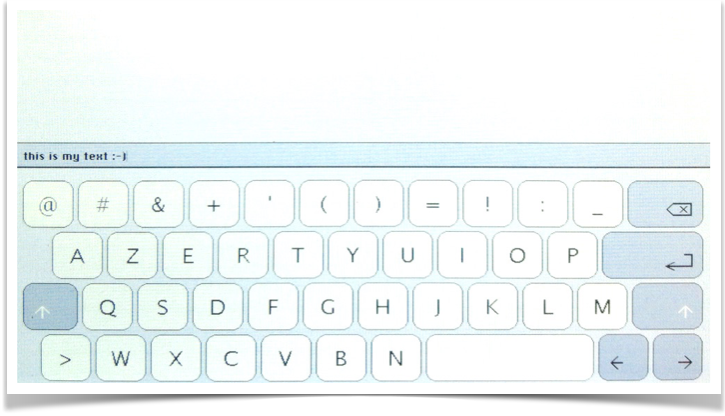
\includegraphics[scale=0.7]{AWFig18.png} 
   \caption{The keyboard view}
   \label{fig:18 }
\end{figure}

~\\

~\\ The Keyboard class contain the following constructor and methods

\begin{lstlisting}[language=Arduinonl]
typedef void (*AWKeyboardCallback)(const String &inText, const int inTag);

void launchKeyboard (const String &inText,
                     const AWInt inMaxLength,
                     AWKeyboardCallback inCallback,
                     const int inTag = -1) ;
\end{lstlisting}

~\\ This example show how to use this keyboard. We need a Label to display the string which will be the result of the use of the keyboard. Then we need an Action which will display this result in the Label when the "return" key of the keyboard will be down. Then we need an Action to displau the keyboard when the user click on a PushButton.

\begin{lstlisting}[language=Arduinonl]
AWLabel *keyboardResult ;

// Action to validate a keyboard entry
void keyboardValidateEntryAction(const String &inText, const int tag)
{
  keyboardResult->setTitle (inText) ;
}

// Action to display the keyboard
void displayKeyboardAction(AWView *sender)
{
  launchKeyboard (keyboardResult->title (), 40, keyboardValidateEntryAction, 0) ;
}

\end{lstlisting}

~\\ Then, in the setup, we create the Label for the result and the PushButton to display the keyboard

\begin{lstlisting}[language=Arduinonl]
  keyboardResult = new AWLabel (AWPoint (0, 0), 500, kAWAlignmentCenter, "") ;
  addCenteredView (keyboardResult) ;
  
  // Push button to display the Keyboard
  AWPushButton *launchKeyboardButton = new AWPushButton (AWRect (20, 20, 150, 40), "Show keyboard");
  launchKeyboardButton->setAction (displayKeyboardAction) ;
  addView (launchKeyboardButton) ;
\end{lstlisting}

~\\ As usual, everything is handled by the loop function :

\begin{lstlisting}[language=Arduinonl]
AWContext::handleTouchAndDisplay () ;
\end{lstlisting}



%%%%%%%%%%%%%%
\newpage
\section{Custom View Examples}

~\\ There is plently of new Arduino Widgets classes  that can be built from the \texttt{AWView} class and from the above existing classes.

~\\ This section describe a few examples which will give you more details on the above existing views and their interactions via the action mecanisms.

~\\ You will find :
\begin{itemize}
\item An Ellipse View
\item A Target View with an arrow
\item A List View that you can fill with the Keyboard View
\item A List View with Badge
\end{itemize}


%%%%%%%%%%%%%%
\newpage
\subsection{The Ellipse custom view}

~\\ This custom view is composed of an Oval which is drawn in a Rectangle. It is defined by a rectangle, a background color and an ellipse color.
~\\
~\\

\begin{figure}[htbp]
   \centering
   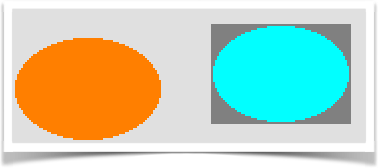
\includegraphics[scale=0.7]{AWFig20.png} 
   \caption{"An Ellipse" custom view}
   \label{fig:20 }
\end{figure}

~\\ The declaration of the EllipseView class is :

\begin{lstlisting}[language=Arduinonl]
class EllipseView : public AWView {
//--- Constructor
  public : EllipseView (const AWRect & inRelativeFrame,
                        const AWColor & inBackColor,
                        const AWColor & inEllipseColor) :
  AWView (inRelativeFrame, inBackColor), 
    mEllipseColor (inEllipseColor) {
  }

//--- Draw
  public : virtual void drawInRegion (const AWRegion & inDrawRegion) const {
  //--- Draw background
    super::drawInRegion (inDrawRegion) ;
  //--- Draw ellipse
    AWRect r = absoluteFrame () ;
    r.inset (1, 1) ;
    AWContext::setColor (mEllipseColor) ;
    r.fillOvalInRegion (inDrawRegion) ;
  }

//--- Private member
  private : AWColor mEllipseColor ;

//--- For calling super class instance methods
   private : typedef AWView super ;
} ;
\end{lstlisting}

~\\ Note that the ellipse is drawn 1 pixel far from the sides of the rectangle.

~\\ In the setup, we create one orange ellipse with no backcolor (we use the argument awkBackColor), and one cyan ellipse with a gray backcolor.

\begin{lstlisting}[language=Arduinonl]
  view = new EllipseView (AWRect (1, 1, 75, 53), awkBackColor , AWColor::orange ()) ;
  addView (view) ;
  view = new EllipseView (AWRect (100, 10, 70, 50), AWColor::gray (), AWColor::cyan ()) ;
  addView (view) ;
\end{lstlisting}

%%%%%%%%%%%%%%
\newpage
\subsection{The Target custom view}

~\\ This example is composed of :
\begin{itemize}
\item 3 concentric circles with different colors
\item An arrow which have reached the center of this target
\item A PushButton to rotate the colors of the target
\end{itemize}

~\\
~\\

\begin{figure}[htbp]
   \centering
   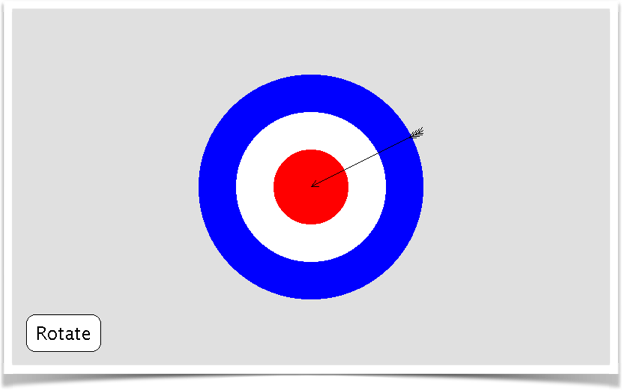
\includegraphics[scale=0.7]{AWFig19.png} 
   \caption{"A Target" custom view}
   \label{fig:19 }
\end{figure}

~\\ First declare the new CustomView class and its functions
~\\

\begin{lstlisting}[language=Arduinonl]
// the CustomView class
class CustomView : public AWView
{
  public : CustomView (const AWRect & inViewFrame);
  public : virtual void drawInRegion (const AWRegion & inRegion) const;
  public : void rotateColors ();

  private : AWColor centerColor;
  private : AWColor mediumColor;
  private : AWColor externalColor;
};

// The CustomView constructor
CustomView::CustomView (const AWRect & inViewFrame) :
AWView(inViewFrame, AWColor::darkGray ()),
centerColor (AWColor::red ()),
mediumColor (AWColor::white ()),
externalColor (AWColor::blue ())
{
}

// The arrow
void drawLines (const AWRegion & inRegion, const AWPoint & inOrigin)
{
  AWPoint p = inOrigin ;
  p.translateBy ( 10, 0 ) ;
  inOrigin.strokeLineInRegion (p, inRegion) ;
  p.translateBy ( -4, 8 ) ;
  inOrigin.strokeLineInRegion (p, inRegion) ;
}

// The drawing of the CustomView class
void CustomView::drawInRegion (const AWRegion & inRegion) const
{
  AWRect viewFrame = absoluteFrame () ;
  AWContext::setColor (externalColor) ;
  viewFrame.fillOvalInRegion (inRegion) ;
  AWInt insetX = viewFrame.size.width / 6 ;
  AWInt insetY = viewFrame.size.height / 6 ;
  AWContext::setColor (mediumColor) ;
  viewFrame.inset (insetX, insetY) ;
  viewFrame.fillOvalInRegion (inRegion) ;  
  AWContext::setColor (centerColor) ;
  viewFrame.inset (insetX, insetY) ;
  viewFrame.fillOvalInRegion (inRegion) ; 

  viewFrame = absoluteFrame () ;
  AWPoint center ;
  center.x = viewFrame.origin.x + viewFrame.size.width / 2 ;
  center.y = viewFrame.origin.y + viewFrame.size.height / 2 ;
  AWPoint tail ;
  tail.x = center.x + viewFrame.size.width / 2 ;
  tail.y = center.y + viewFrame.size.height / 4 ;
  AWContext::setColor (AWColor::black ()) ;
  center.strokeLineInRegion (tail, inRegion) ;
  drawLines (inRegion, center) ;
  center.translateBy (viewFrame.size.width / 2 - 20, viewFrame.size.width / 4 - 10) ; 
  for (int i = 0 ; i < 4 ; i++) {
    drawLines (inRegion, center) ;
    center.translateBy (4, 2) ;
  }
}

// the color rotation function of the CustomView class
void CustomView::rotateColors ()
{
  AWColor centerSave = centerColor ;
  centerColor = mediumColor ;
  mediumColor = externalColor ;
  externalColor = centerSave ;
  setNeedsDisplay () ;
}

// The targetView object pointer
CustomView * targetView ;

// The color rotation function of the targetView object
void rotate (AWView * sender)
{
  targetView->rotateColors () ;
}
\end{lstlisting}


~\\ Then create the elements in the \texttt{setup}
~\\

\begin{lstlisting}[language=Arduinonl]
  // create the target view centered on screen
  targetView = new CustomView(AWRect (0, 0, 300, 300)) ;
  addCenteredView (targetView) ;

  // create the button to rotate colors
  AWPushButton * pushToRotate = new AWPushButton (AWRect (20, 20, 100, 50), "Rotate", AWFont (Lucida_Grande24)) ;
  pushToRotate->setAction (rotate) ;
  addView (pushToRotate) ;
\end{lstlisting}


%%%%%%%%%%%%%%
\newpage
\subsection{The Keyboard and List example}

~\\ This example is composed of :
\begin{itemize}
\item An AWList View
\item An AWPushButton to add an element
\item An AWPushButton to delete an element
\item An AWKeyboard to compose and enter an element
\end{itemize}

~\\ The following figures show the list :
\begin{itemize}
\item With the keyboard to enter an element
\item With the buttons to add or remove an element
\end{itemize}


\begin{figure}[htbp]
   \centering
   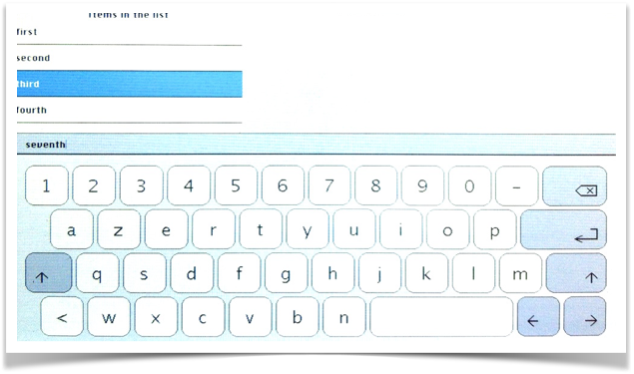
\includegraphics[scale=0.55]{AWFig21.png} 
   \caption{Keyboard and List views}
   \label{fig:21 }
\end{figure}

\begin{figure}[htbp]
   \centering
   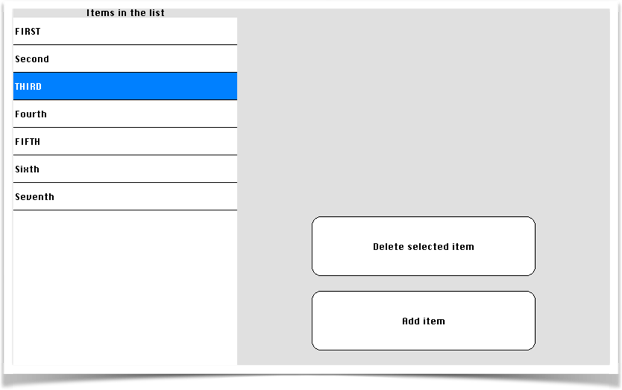
\includegraphics[scale=0.55]{AWFig22.png} 
   \caption{The List}
   \label{fig:22 }
\end{figure}

~\\ To program this example, you declare the objects and actions :
~\\

\begin{lstlisting}[language=Arduinonl]
//--- List View
AWListView * listView ;

// delete item button, enabled only if listView is not empty
AWPushButton * delButton ;

// Action to validate a keyboard entry
void keyboardValidateEntryAction(const String &inText, const int tag)
{
  listView->append (inText) ;
  delButton->setEnabled (true) ;
}

//--- button to add an item to the list action
void addItemAction (AWView * inSender)
{
  launchKeyboard ("", 40, keyboardValidateEntryAction, 0) ;
}

//--- button to remove the selected item from the list action
void delItemAction (AWView * inSender)
{
  listView->removeItemAtIndex (listView->selectedItemIndex ()) ;
  if (listView->count () == 0) {
    delButton->setEnabled (false) ;
  }
}
\end{lstlisting}

~\\ Then you create the objects in the \texttt{setup}.
~\\

\begin{lstlisting}[language=Arduinonl]
  // Create the listView
  listView = new AWListView ( AWRect (0, 0, 300, 480), "Items in the list") ;
  addView (listView) ;
  // Create the "Add item" PushButton
  AWPushButton * addButton = new AWPushButton(AWRect (400, 20, 300, 80), "Add item") ;
  addButton->setAction (addItemAction) ;
  addView (addButton) ;
  // Create the "Delete selected item" PushButton
  delButton = new AWPushButton(AWRect (400, 120, 300, 80), "Delete selected item") ;
  delButton->setEnabled (false) ;
  delButton->setAction (delItemAction) ;
  addView (delButton) ;
\end{lstlisting}

%%%%%%%%%%%%%%
\newpage
\section{A List View with Badge}

~\\ This example is composed of :
\begin{itemize}
\item An AWListView named "My List"
\item An AWSwitch "Has Badge"
\item An AWPushButton "Remove"
\item An Alert dialog
\end{itemize}

~\\ This figure show 4 states of this exemple, from left to right :
\begin{itemize}
\item The initial list with first element selected
\item The 3rd element selected with a click on it
\item After removing the "alien" element
\item After selecting and clicking the switch "Has Badge" of 3 elements
\end{itemize}


\begin{figure}[htbp]
   \centering
   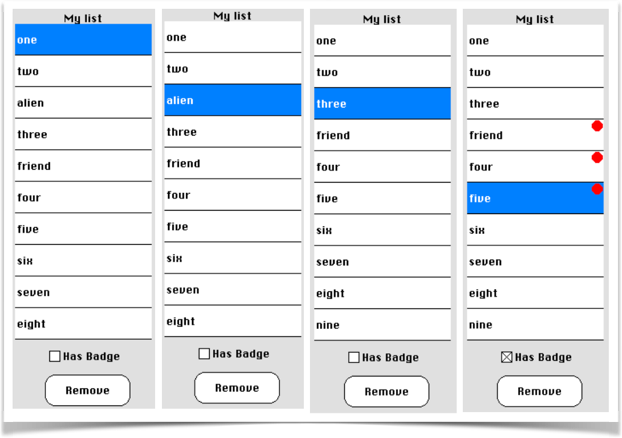
\includegraphics[scale=0.6]{AWFig30.png} 
   \caption{Managing a list with badge}
   \label{fig:30 }
\end{figure}

~\\ And this figure show the Alert dialog when clicking the "Remove" PushButton

\begin{figure}[htbp]
   \centering
   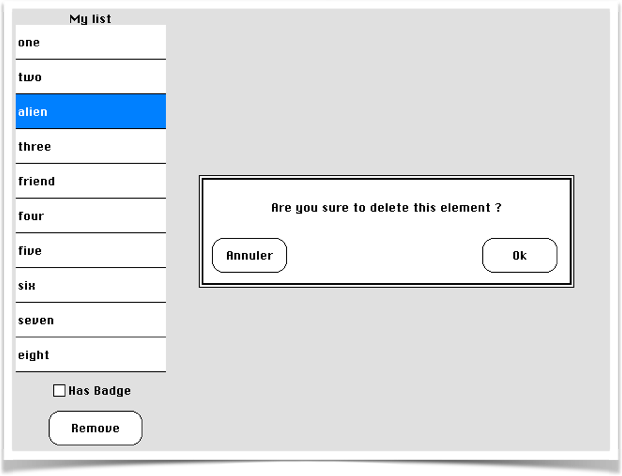
\includegraphics[scale=0.60]{AWFig31.png} 
   \caption{Alert when removing an element of the list}
   \label{fig:22 }
\end{figure}

~\\ Before the setup, we declare the following objects :

\begin{lstlisting}[language=Arduinonl]
static AWListView * gListView ;
static AWPushButton * gRemoveItemLabel ;
static AWSwitch * gHasBadgeSwitch ;
\end{lstlisting}


~\\ Then we declare the following functions

\begin{lstlisting}[language=Arduinonl]
// The action when selecting an element in the list
static void listSelectionAction (AWView * inSender) {
    const AWInt selectedItemIndex = gListView->selectedItemIndex () ;
    gRemoveItemLabel->setEnabled (selectedItemIndex >= 0) ;
    gHasBadgeSwitch->setEnabled (selectedItemIndex >= 0) ;
    gHasBadgeSwitch->setChecked (gListView->hasBadgeAtIndex (selectedItemIndex)) ;
}
// The action when removing an element
static void listRemoveAction (AWView * inSender) {
    gListView->removeItemAtIndex (gListView->selectedItemIndex ()) ;
}
// The action when clicking in the "Remove" button
static void removeButtonAction (AWView * inSender) {
    presentAlert ("Are you sure to delete this element ?", NULL, listRemoveAction, -1) ;
}
// The action when clicking in the "Has Badge" switch
static void hasBadgeSwitchAction (AWView * inSender) {
    const AWInt selectedItemIndex = gListView->selectedItemIndex () ;
    if (selectedItemIndex >= 0) {
        gListView->setBadgeAtIndex (selectedItemIndex, gHasBadgeSwitch->checked ()) ;
    }
}
\end{lstlisting}

~\\ Then we create the objects in the setup :

\begin{lstlisting}[language=Arduinonl]
  // The "Remove" PushButton
  gRemoveItemLabel = new AWPushButton (AWPoint (40, 25), 100, "Remove") ;
  gRemoveItemLabel->setAction (removeButtonAction) ;
  addView (gRemoveItemLabel) ;
  // The empty list of elements in a rectangle that can limit the display of the list
  gListView = new AWListView (AWRect (5, 90, 160, 383), "My list") ;
  addView (gListView) ;
  // The elements which are appended to the liste
  gListView->append ("one") ;
  gListView->append ("two") ;
  gListView->append ("alien") ;
  gListView->append ("three") ;
  gListView->append ("friend") ;
  gListView->append ("four") ;
  gListView->append ("five") ;
  gListView->append ("six") ;
  gListView->append ("seven") ;
  gListView->append ("eight") ;
  gListView->append ("nine") ;
  gListView->append ("ten") ;
  gListView->append ("eleven") ;
  gListView->append ("12") ;
  gListView->append ("13") ;
  gListView->append ("14") ;
  // The "Has Badge" Switch
  gHasBadgeSwitch = new AWSwitch (AWPoint (45, 65), "Has Badge") ;
  gHasBadgeSwitch->setAction (hasBadgeSwitchAction) ;
  addView (gHasBadgeSwitch) ;
  // Start the action when selecting an element in the list
  gListView->setAction (listSelectionAction) ;
\end{lstlisting}


\begin{lstlisting}[language=Arduinonl]

\end{lstlisting}

%%%%%%%%%%%%%%
\newpage
\section{The next steps of \emph{ArduinoWidgets}}

~\\ With this AroduinoWidgets toolbox, you can create custom views for your project and we will be pleased to add some of them in this library if that make sens.

~\\ 

~\\


%%%%%%%%%%%%%%%%%%%%%%%%%%%%%%%%%%%
\newpage
\section{The calibration of the Touch screen} 

~\\ There is a function which can be used to calibrate a new screen. It must be used only once preferably by a stand alone program, in the \texttt{setup}.

\begin{lstlisting}[language=Arduinonl]
//---------------------- Calibrate touch
//  AWContext::calibrateTouch () ;
\end{lstlisting}

~\\ This program is a help to determine the following constants :

\begin{lstlisting}[language=Arduinonl]
const float xA =  310.0 ; // 571.0 ;
const float yA =  116.0 ; // 963.0 ;

const float xB = 3811.0 ; // 488.0 ;
const float yB =  113.0 ; // 3001.0 ;

const float xC = 3814.0 ; // 3526.0 ;
const float yC = 3936.0 ; // 3349.0 ;

const float xD =  362.0 ; // 3519.0 ;
const float yD = 3938.0 ; // 698.0 ;
\end{lstlisting}

~\\ Another help for debugging is to add the folliowing lines in your \texttt{setup} :

\begin{lstlisting}[language=Arduinonl]
//---------------------- Debug touch
// For enabling touch debug, uncomment the following line
//  AWContext::debugTouch (AWColor::red ()) ;
// if this line is uncommented, when a touch occurs, event is not sent to widgets, but a small square of the given
// color is drawn at touch location. This enables you to adjust the convertTouchPointToScreenPoint function
// (see convertTouchPointToScreenPoint.cpp) that converts touch location to actual screen location.
\end{lstlisting}

~\\


%-----------------------------------------------------------------------------------------------------------------------*
%   F I N    D U    D O C U M E N T                                                                                     *
%-----------------------------------------------------------------------------------------------------------------------*

\end{document}
